\documentclass{article}

% --- packages ---
\usepackage[utf8]{inputenc}
\usepackage[T1]{fontenc}
\usepackage{lmodern}
\usepackage{textcomp}
\usepackage{amsmath,amssymb,amsfonts,amsthm}
\usepackage{graphicx}
\usepackage{booktabs}
\usepackage{array}
\usepackage{longtable}
\usepackage{tabularx}
\usepackage{ltablex}
\keepXColumns
\usepackage{float}
\usepackage{xcolor}
\usepackage[margin=1in]{geometry}
\usepackage{enumitem}
\usepackage{calc}
\usepackage{hyperref}
\hypersetup{colorlinks=true,linkcolor=blue!50!black,citecolor=blue!50!black,urlcolor=blue!50!black}

% pandoc shims
\providecommand{\tightlist}{\setlength{\itemsep}{0pt}\setlength{\parskip}{0pt}}
\providecommand{\real}[1]{#1}

% Make verbatim a little smaller and allow page breaks inside
\usepackage{fancyvrb}
\fvset{fontsize=\small,frame=single,framerule=0pt,xleftmargin=0pt}
\RecustomVerbatimEnvironment{verbatim}{Verbatim}{fontsize=\small,frame=lines,framerule=0.4pt,framesep=4pt,xleftmargin=0pt}

% --- Python syntax highlighting via listings ---
\usepackage{listings}
\definecolor{pyBg}{rgb}{0.97,0.97,0.97}
\definecolor{pyKw}{rgb}{0.00,0.00,0.70}
\definecolor{pyStr}{rgb}{0.80,0.20,0.10}
\definecolor{pyCom}{rgb}{0.10,0.55,0.10}
\definecolor{pyNum}{rgb}{0.50,0.10,0.60}
\definecolor{pyFrame}{rgb}{0.75,0.75,0.75}
\lstdefinestyle{pythonstyle}{
  language=Python,
  backgroundcolor=\color{pyBg},
  basicstyle=\ttfamily\footnotesize,
  keywordstyle=\color{pyKw}\bfseries,
  stringstyle=\color{pyStr},
  commentstyle=\color{pyCom}\itshape,
  numberstyle=\color{pyNum},
  identifierstyle=\color{black},
  showstringspaces=false,
  breaklines=true,
  breakatwhitespace=true,
  columns=fullflexible,
  keepspaces=true,
  tabsize=4,
  frame=single,
  rulecolor=\color{pyFrame},
  framesep=4pt,
  framerule=0.4pt,
  xleftmargin=4pt,
  xrightmargin=4pt,
  extendedchars=true,
  inputencoding=utf8,
  literate=%
    {~}{{$\sim$}}1
    {±}{{$\pm$}}1
    {²}{{${}^2$}}1
    {β}{{$\beta$}}1
    {—}{{---}}1,
  upquote=true,
}
\lstset{style=pythonstyle}

% --- Unicode passthrough for text-mode glyphs that appear in tables/prose ---
\DeclareUnicodeCharacter{2713}{\ensuremath{\checkmark}}
\DeclareUnicodeCharacter{2717}{\ensuremath{\times}}
\DeclareUnicodeCharacter{2192}{\ensuremath{\rightarrow}}
\DeclareUnicodeCharacter{2208}{\ensuremath{\in}}
\DeclareUnicodeCharacter{2212}{\ensuremath{-}}
\DeclareUnicodeCharacter{223C}{\ensuremath{\sim}}
\DeclareUnicodeCharacter{2248}{\ensuremath{\approx}}
\DeclareUnicodeCharacter{2261}{\ensuremath{\equiv}}
\DeclareUnicodeCharacter{2014}{---}
\DeclareUnicodeCharacter{00B1}{\ensuremath{\pm}}
\DeclareUnicodeCharacter{00B2}{\ensuremath{{}^2}}
\DeclareUnicodeCharacter{00D7}{\ensuremath{\times}}
\DeclareUnicodeCharacter{03B2}{\ensuremath{\beta}}

% --- theorem environments ---
\newtheorem{definition}{Definition}
\newtheorem{proposition}{Proposition}
\newtheorem{remark}{Remark}

% Title metadata
\title{A Practitioner's Guide to Correlation, Dependence, and Feature Importance\\
\large{Classical correlations, information-theoretic dependence, geometric/kernel measures, and feature-importance metrics}}

\author{
  Nikolas Markou \\
  \texttt{nikolasmarkou@gmail.com}
}

\date{}

\let\oldsection\section
\renewcommand{\section}{\clearpage\oldsection}

\begin{document}

\maketitle

\begin{abstract}
This guide is an integrated, self-contained reference covering the four large families of metrics that quantify the relationship between variables in modern data analysis: classical correlation coefficients (Pearson, Spearman, Kendall, point-biserial, $\phi$, Cram\'er's $V$, tetrachoric/polychoric), information-theoretic dependence (mutual information, MIC, NMI, transfer entropy, CMI), modern geometric and kernel-based independence criteria (distance correlation, Brownian covariance, kernel-CCA, HSIC, Chatterjee's $\xi$), and the dominant families of feature-importance metrics used in machine learning (SHAP, permutation importance, LIME, PDP/ICE, plus tree-specific impurity-based importances). Each metric is documented with its definition, derivation, asymptotic properties, code recipe, canonical pitfalls, and guidance on when to use --- and when not to. A master comparison table classifies every measure along five properties (range, symmetry, captures non-linearity, requires distributional assumptions, computational cost), a prerequisites primer brings the reader up to speed on the supporting probability and statistics, and three appendices catalogue reference implementations and provide a fully worked numerical walkthrough.
\end{abstract}

\tableofcontents
\clearpage


\section{Introduction}\label{introduction}

Asking \emph{"how strongly are two variables related?"} sounds like a
single question. It is not. The answer depends on \textbf{what you mean
by related} (linear? monotonic? functional? statistical?), \textbf{what
kind of variables you have} (continuous, ordinal, binary, multivariate,
time-indexed?), \textbf{what you intend to do with the answer} (rank
features? test a hypothesis? interpret a black-box model? estimate a
causal effect?), and \textbf{what assumptions you are willing to make}
about the joint distribution.

Over the last 130 years the statistical literature has produced a
sprawling menagerie of correlation coefficients, dependence measures,
and importance scores. They are not interchangeable.
Pearson\textquotesingle s \(r\) can be zero for a deterministic
relationship; mutual information cannot distinguish positive from
negative association; SHAP gives you per-prediction credit but tells you
nothing about the data-generating process; Gini importance is biased
toward high-cardinality features; and a permutation feature importance
computed on training data is closer to a measure of memorisation than of
generalisation. Each measure encodes a different theory of what
"association" \emph{means}, and the wrong choice can flip the
qualitative conclusion of an analysis.

A guiding distinction will resurface throughout. \textbf{Correlation
coefficients} are summary statistics of the joint distribution of
\emph{raw variables}. \textbf{Feature importance metrics} are summary
statistics of \emph{a model fitted to those variables}. A feature can be
enormously important to a particular model without being statistically
associated with the target after controlling for the rest, and vice
versa. Confusing the two is one of the most common mistakes in applied
machine learning, and it has cost people money, reputations, and the
occasional clinical trial.

The structure of the guide mirrors the historical and mathematical arc
of the field:

\begin{itemize}
\tightlist
\item
  \textbf{Part I} covers the classical and rank-based coefficients
  (Pearson, Spearman, Kendall, point-biserial, \(\phi\),
  Cramér\textquotesingle s \(V\), tetrachoric/polychoric). These are the
  workhorses of nineteenth- and early-twentieth-century statistics and
  remain the most-used measures by an enormous margin.
\item
  \textbf{Part II} introduces information-theoretic dependence (mutual
  information, MIC, NMI, transfer entropy, conditional MI).
  Shannon\textquotesingle s framework gave statisticians a \emph{fully
  general} notion of dependence, at the cost of new estimation
  difficulties.
\item
  \textbf{Part III} covers the modern geometric, kernel, and
  rank-functional measures (distance correlation, Brownian covariance,
  KCCA, HSIC, Chatterjee\textquotesingle s \(\xi\)). These resolve many
  of MI\textquotesingle s estimation pains while preserving the "detects
  any dependence" property.
\item
  \textbf{Part IV} turns to model-agnostic feature importance (SHAP,
  permutation importance, LIME, PDP/ICE). The questions change: we are
  no longer summarising the joint distribution of raw variables, but the
  behaviour of a fitted model.
\item
  \textbf{Part V} covers tree-specific and embedded metrics (MDI/Gini,
  MDA, gain/split/cover in boosting, LASSO/Ridge coefficients). These
  are cheap, ubiquitous, and frequently misinterpreted.
\end{itemize}

Each metric section follows a uniform template --- formal definition,
derivation, intuition, properties, asymptotic theory, estimation
algorithm, runnable code snippet, worked numerical example, pitfalls,
when-to-use / when-not-to-use, cross-references --- so you can navigate
by metric without reading top-to-bottom. The cross-cutting themes at the
end consolidate ideas (significance testing, multiplicity, confounding)
that apply to every measure in the document.

A note on style: this is a \emph{practitioner\textquotesingle s} guide.
It is mathematically rigorous where rigor is illuminating but stops
short of measure-theoretic foundations. References to deeper material
are flagged inline and collected in Appendix C.

\begin{center}\rule{0.5\linewidth}{0.5pt}\end{center}

\section{How to Read This Guide}\label{how-to-read-this-guide}

Three reading modes are supported:

\begin{enumerate}
\def\labelenumi{\arabic{enumi}.}
\tightlist
\item
  \textbf{Linear}. Read top to bottom. This works because the parts are
  ordered roughly by mathematical sophistication and by the
  chronological development of the ideas. You will end up with a
  coherent map of the entire landscape.
\item
  \textbf{Per-metric}. Use the TOC and the master comparison table to
  find the metric you need; each metric section is self-contained except
  for cross-references that are explicitly hyperlinked.
\item
  \textbf{By question}. The decision tree under
  \hyperref[cross-cutting-themes]{Choosing a Measure} and the
  \hyperref[common-confusions-and-how-to-resolve-them]{Common
  Confusions} section route you from a real-world question ("my data are
  ordinal, how do I correlate them?") to the right metric.
\end{enumerate}

The \hyperref[prerequisites-primer]{Prerequisites Primer} is
intentionally placed before the technical content. If a term in a later
section is unfamiliar, the primer almost certainly defines it; the
glossary at the end is a one-line fallback.

\begin{center}\rule{0.5\linewidth}{0.5pt}\end{center}

\section{Notation and Conventions}\label{notation-and-conventions}

{\def\LTcaptype{none} % do not increment counter
\begin{longtable}[]{@{}ll@{}}
\toprule\noalign{}
Symbol & Meaning \\
\midrule\noalign{}
\endhead
\bottomrule\noalign{}
\endlastfoot
\(X, Y, Z\) & Random variables (capital letters); \(X\) may be a vector
\(\mathbf{X} \in \mathbb{R}^p\). \\
\(x_i, y_i\) & Realised values of \(X, Y\) in a sample of size \(n\),
\(i = 1, \dots, n\). \\
\(\bar{x}, \bar{y}\) & Sample means
\(\bar{x} = \tfrac{1}{n}\sum_i x_i\). \\
\(s_x, s_y\) & Sample standard deviations (with Bessel\textquotesingle s
correction \(n-1\) in the denominator unless noted). \\
\(F_X, p_X\) & Cumulative distribution function (CDF) and probability
density / mass function (PDF/PMF) of \(X\). \\
\(H(X)\) & Shannon entropy of \(X\) (differential entropy if \(X\) is
continuous). \\
\(I(X;Y)\) & Mutual information between \(X\) and \(Y\). \\
\(D_{\mathrm{KL}}(p \,|\, q)\) & Kullback--Leibler divergence of \(q\)
from \(p\). \\
\(R_i, Q_i\) & Ranks of \(x_i\) and \(y_i\) (smallest = rank 1; ties
handled by average rank unless noted). \\
\(\mathbb{1}[\cdot]\) & Indicator function. \\
\(|\cdot|\) & Euclidean norm on \(\mathbb{R}^d\) (or RKHS norm
\(|\cdot|_\mathcal{H}\) where specified). \\
\(\mathcal{H}, k\) & A reproducing kernel Hilbert space and its kernel
function. \\
\(f, \hat{f}\) & A model (function) and its empirical fit. \\
\(\mathcal{L}\) & A loss function. \\
\(\mathbb{E}, \mathrm{Var}, \mathrm{Cov}\) & Expectation, variance,
covariance operators. \\
\(\Phi, \varphi\) & Standard normal CDF and characteristic function
respectively (context-dependent). \\
\(\perp\) & Statistical independence: \(X \perp Y\) means
\(p_{XY} = p_X p_Y\). \\
\(\binom{n}{k}\) & Binomial coefficient \(n! / (k!(n-k)!)\). \\
\(\to_p, \to_d\) & Convergence in probability, convergence in
distribution. \\
\end{longtable}
}

All logarithms in information-theoretic sections are natural unless we
explicitly write \(\log_2\) (in which case the unit is bits rather than
nats). Code snippets assume Python 3.11+, NumPy, SciPy, and scikit-learn
unless stated otherwise.

\begin{center}\rule{0.5\linewidth}{0.5pt}\end{center}

\section{Prerequisites Primer}\label{prerequisites-primer}

This section is for readers who want a refresher before encountering the
dependence measures. Skim it once or skip and return as needed.

\subsection{P1. Random variables, expectations, and
moments}\label{p1-random-variables-expectations-and-moments}

A random variable \(X\) is a measurable function from a probability
space to \(\mathbb{R}\) (or \(\mathbb{R}^d\)). It is characterised by
its \textbf{distribution}, summarised either by a CDF
\(F_X(x) = P(X \leq x)\) or, where it exists, a density
\(p_X(x) = F_X'(x)\).

The \textbf{expectation} \(\mathbb{E}[X] = \int x \, dF_X(x)\) is the
population mean; the \textbf{variance}
\(\mathrm{Var}(X) = \mathbb{E}[(X - \mathbb{E}[X])^2]\) measures spread.
\textbf{Covariance} between two variables is \[
\mathrm{Cov}(X, Y) = \mathbb{E}[(X - \mathbb{E}[X])(Y - \mathbb{E}[Y])] = \mathbb{E}[XY] - \mathbb{E}[X]\mathbb{E}[Y].
\] Covariance is unbounded; \textbf{correlation} is the scale-free
version, \(\rho_{XY} = \mathrm{Cov}(X, Y) / (\sigma_X \sigma_Y)\).

\textbf{Moments} of \(X\) are \(m_k = \mathbb{E}[X^k]\) (raw) or
\(\mu_k = \mathbb{E}[(X - \mathbb{E}[X])^k]\) (central). The third
central moment relates to skewness, the fourth to kurtosis. A
distribution is \emph{characterised} by its moments if its
moment-generating function \(M_X(t) = \mathbb{E}[e^{tX}]\) exists in a
neighbourhood of zero --- but distributions with all finite moments need
not be uniquely determined by them (the log-normal is a classic
counterexample). The characteristic function below sidesteps this issue.

\subsection{P2. Entropy, cross-entropy, KL
divergence}\label{p2-entropy-cross-entropy-kl-divergence}

\textbf{Shannon entropy} of a discrete random variable with PMF \(p\) on
alphabet \(\mathcal{X}\): \[
H(X) = -\sum_{x \in \mathcal{X}} p(x) \log p(x).
\] The unit is \emph{nats} with \(\log = \ln\), \emph{bits} with
\(\log_2\). \(H(X) \geq 0\), with \(H(X) = 0\) iff \(X\) is
deterministic, and \(H(X) \leq \log |\mathcal{X}|\) with equality at
uniform distribution. Intuitively, \(H(X)\) is the average number of
nats needed to optimally encode a draw from \(X\).

For continuous \(X\) with density \(p\) the \textbf{differential
entropy} is \(h(X) = -\int p(x) \log p(x)\, dx\). Differential entropy
can be \emph{negative} (e.g. a uniform on \([0, 0.1]\)) and is not
invariant under change of variables --- these quirks matter when
interpreting MI estimates.

\textbf{Joint and conditional entropy}:
\(H(X, Y) = -\sum p(x, y) \log p(x, y)\) and
\(H(Y \mid X) = H(X, Y) - H(X)\). The \textbf{chain rule} is
\(H(X, Y) = H(X) + H(Y \mid X)\).

\textbf{Kullback--Leibler divergence} (relative entropy) between two
distributions \(p, q\) on the same support: \[
D_{\mathrm{KL}}(p \,\|\, q) = \sum_x p(x) \log \frac{p(x)}{q(x)}.
\] Asymmetric (\(D_{\mathrm{KL}}(p\|q) \neq D_{\mathrm{KL}}(q\|p)\)),
non-negative, zero iff \(p = q\) almost everywhere. KL is \emph{not} a
metric (no triangle inequality, no symmetry) but is the canonical
"distance from \(p\) to \(q\)" in information theory.

\textbf{Mutual information} is the KL divergence between the joint and
the product of marginals: \[
I(X; Y) = D_{\mathrm{KL}}\big(p_{XY} \,\|\, p_X p_Y\big) = H(X) + H(Y) - H(X, Y).
\]

\subsection{P3. Characteristic
functions}\label{p3-characteristic-functions}

The \textbf{characteristic function} of \(X\) is
\(\varphi_X(t) = \mathbb{E}[e^{itX}]\) for \(t \in \mathbb{R}\). Three
facts to remember:

\begin{enumerate}
\def\labelenumi{\arabic{enumi}.}
\tightlist
\item
  \(\varphi_X\) \emph{always} exists and uniquely determines the
  distribution.
\item
  Independence is equivalent to factorisation:
  \(X \perp Y \iff \varphi_{X, Y}(t, s) = \varphi_X(t)\, \varphi_Y(s)\)
  for all \(t, s\).
\item
  Distance correlation (Part III) is built directly on this
  characterisation: it measures the \(L^2\) distance between
  \(\varphi_{XY}\) and \(\varphi_X \varphi_Y\) in a specific weighted
  sense. This is the entire reason dCor is an \emph{if and only if} test
  of independence while Pearson is not.
\end{enumerate}

\subsection{P4. Reproducing kernel Hilbert spaces
(RKHS)}\label{p4-reproducing-kernel-hilbert-spaces-rkhs}

A \textbf{kernel} is a symmetric positive-definite function
\(k: \mathcal{X} \times \mathcal{X} \to \mathbb{R}\) --- that is, for
any finite collection \(x_1, \dots, x_n \in \mathcal{X}\), the Gram
matrix \(K_{ij} = k(x_i, x_j)\) is positive semi-definite. Examples:
linear \(k(x, y) = \langle x, y \rangle\); polynomial
\(k(x, y) = (\langle x, y \rangle + c)^d\); Gaussian RBF
\(k(x, y) = \exp(-\|x - y\|^2 / 2\sigma^2)\); Laplace
\(k(x, y) = \exp(-\|x - y\|/\sigma)\).

To each kernel corresponds a unique Hilbert space \(\mathcal{H}\) of
functions \(\mathcal{X} \to \mathbb{R}\) --- the \textbf{RKHS} --- with
the \emph{reproducing property}:
\(f(x) = \langle f, k(\cdot, x) \rangle_\mathcal{H}\). The map
\(\phi: x \mapsto k(\cdot, x)\) is the \textbf{feature map}; it embeds
\(\mathcal{X}\) into \(\mathcal{H}\), and inner products in
\(\mathcal{H}\) can be computed via the kernel (the \emph{kernel
trick}): \(\langle \phi(x), \phi(y) \rangle_\mathcal{H} = k(x, y)\).

A kernel is \textbf{characteristic} if the mean embedding
\(\mu_P = \mathbb{E}_{X \sim P}[\phi(X)]\) is injective in \(P\), i.e.
\(\mu_P = \mu_Q \Rightarrow P = Q\). The Gaussian RBF is characteristic
on \(\mathbb{R}^d\). This property is what allows HSIC with an RBF
kernel to be a true independence test.

\subsection{P5. U-statistics and
V-statistics}\label{p5-u-statistics-and-v-statistics}

Many estimators in this guide are written as averages over \(k\)-tuples
of observations rather than over single observations. A
\textbf{U-statistic} of order \(k\) with symmetric kernel
\(h: \mathcal{X}^k \to \mathbb{R}\) is \[
U_n = \binom{n}{k}^{-1} \sum_{i_1 < i_2 < \dots < i_k} h(x_{i_1}, \dots, x_{i_k}).
\] \textbf{V-statistics} allow repeated indices:
\(V_n = n^{-k}\sum_{i_1, \dots, i_k} h(x_{i_1}, \dots, x_{i_k})\).
U-statistics are unbiased; V-statistics are biased but often simpler.
The bias-corrected distance covariance estimator (Part III, §13) is a
U-statistic; the original 2007 estimator is a V-statistic.

Hoeffding\textquotesingle s central limit theorem: under mild
conditions, \(\sqrt{n}(U_n - \theta) \to_d \mathcal{N}(0, k^2 \zeta_1)\)
where \(\zeta_1\) is the variance of the first conditional projection.
This is the engine behind asymptotic distributions for dCor and HSIC.

\subsection{P6. Bootstrap, permutation,
jackknife}\label{p6-bootstrap-permutation-jackknife}

Three resampling tools:

\begin{itemize}
\tightlist
\item
  \textbf{Bootstrap}: sample \(n\) observations \emph{with replacement}
  from the data, recompute the statistic, repeat \(B\) times. The
  empirical distribution of the bootstrap statistics approximates the
  sampling distribution. Used for \textbf{confidence intervals}
  (percentile, BCa, basic).
\item
  \textbf{Permutation}: shuffle one variable\textquotesingle s values
  across rows, recompute the statistic. Under \(H_0: X \perp Y\), all
  permutations are equally likely; the empirical distribution of
  permuted statistics is the exact null distribution. Used for
  \textbf{hypothesis tests}.
\item
  \textbf{Jackknife}: leave-one-out replicates; recompute the statistic
  on each \(n-1\) subset. Older and less powerful than the bootstrap;
  mainly used for \textbf{bias estimation}.
\end{itemize}

For time series, replace plain bootstrap/permutation with \textbf{block
bootstrap} to preserve autocorrelation.

\subsection{P7. Copulas}\label{p7-copulas}

Sklar\textquotesingle s theorem (1959): any multivariate CDF \(F_{XY}\)
can be written as \(F_{XY}(x, y) = C(F_X(x), F_Y(y))\) where \(C\) is a
\textbf{copula} --- a CDF on \([0, 1]^2\) with uniform marginals. The
copula captures the \emph{dependence structure}, separated from the
marginals.

Spearman\textquotesingle s \(\rho\) and Kendall\textquotesingle s
\(\tau\) are functionals of the copula alone, which is why they are
invariant under monotonic marginal transformations.
Pearson\textquotesingle s \(r\) depends on both the copula and the
marginals. Polychoric correlation assumes a Gaussian copula.

\subsection{P8. Granger causality and
DAGs}\label{p8-granger-causality-and-dags}

\textbf{Granger causality} (Granger 1969): \(X\) Granger-causes \(Y\) if
past values of \(X\) improve the prediction of \(Y\) beyond what is
achievable from past values of \(Y\) alone. In the linear-Gaussian
setting this is a comparison of nested VAR models. The
information-theoretic generalisation is \textbf{transfer entropy} (§11).

\textbf{Directed acyclic graphs (DAGs)} in the Pearl-style causal
framework represent causal relationships among variables as a graph in
which an edge \(X \to Y\) encodes a direct causal effect. The
\textbf{d-separation} criterion translates graph structure into
conditional independence claims about the data. Algorithms like PC and
FCI use conditional-independence tests (often based on partial
correlation, KCIT, or CMI) to learn the DAG skeleton from data.

A pointed caution: every metric in this guide measures
\emph{statistical} dependence in observed data. None of them measure
interventional causal effect on their own. Combining them with the DAG
framework and assumptions like \emph{causal faithfulness} and \emph{no
unobserved confounders} yields causal claims; without those assumptions,
you have only association.

\subsection{P9. Shapley values from cooperative game
theory}\label{p9-shapley-values-from-cooperative-game-theory}

A \textbf{cooperative game} is a pair \((N, v)\) where
\(N = \{1, \dots, p\}\) is the player set and \(v: 2^N \to \mathbb{R}\)
is the value function with \(v(\emptyset) = 0\). The \textbf{Shapley
value} of player \(i\) is \[
\phi_i = \sum_{S \subseteq N \setminus \{i\}} \frac{|S|!\,(p - |S| - 1)!}{p!} \left[ v(S \cup \{i\}) - v(S) \right].
\] This is the \emph{unique} payoff vector satisfying four axioms:

\begin{enumerate}
\def\labelenumi{\arabic{enumi}.}
\tightlist
\item
  \textbf{Efficiency}: \(\sum_i \phi_i = v(N)\).
\item
  \textbf{Symmetry}: if \(v(S \cup \{i\}) = v(S \cup \{j\})\) for all
  \(S\) not containing \(i, j\), then \(\phi_i = \phi_j\).
\item
  \textbf{Dummy / null player}: if \(v(S \cup \{i\}) = v(S)\) for all
  \(S\), then \(\phi_i = 0\).
\item
  \textbf{Additivity}: for two games \(v_1, v_2\) on the same players,
  \(\phi_i(v_1 + v_2) = \phi_i(v_1) + \phi_i(v_2)\).
\end{enumerate}

In SHAP (§18) the "players" are features and \(v(S)\) is the
model\textquotesingle s expected output when only features in \(S\) are
known.

\begin{center}\rule{0.5\linewidth}{0.5pt}\end{center}

\section{The Five Properties That Distinguish Dependence
Measures}\label{the-five-properties-that-distinguish-dependence-measures}

A short checklist that distinguishes the dependence measures at a
glance. For a candidate measure \(D(X, Y)\):

\begin{enumerate}
\def\labelenumi{\arabic{enumi}.}
\tightlist
\item
  \textbf{Range.} Bounded (\([-1, 1]\) or \([0, 1]\)) or unbounded
  (\([0, \infty)\))? Bounded measures are easier to compare across
  datasets; unbounded ones often have a more natural
  information-theoretic interpretation.
\item
  \textbf{Sign.} Does \(D\) distinguish positive from negative
  association, or only the strength? Pearson, Spearman, Kendall do; MI,
  dCor, HSIC, MIC do not.
\item
  \textbf{Independence characterisation.} Is
  \(D(X, Y) = 0 \iff X \perp Y\)? Pearson is famously \emph{not} (it
  only equals zero under linear non-association); dCor, HSIC with a
  characteristic kernel, MI, and Chatterjee\textquotesingle s \(\xi\)
  \emph{are}.
\item
  \textbf{Invariance.} Under what transformations is \(D\) unchanged?
  Pearson under affine transforms; Spearman/Kendall/\(\xi\) under
  strictly monotonic transforms of \(X\) and \(Y\) separately; MI under
  any \emph{invertible} transform; dCor and HSIC under orthogonal
  transforms (kernel-choice dependent).
\item
  \textbf{Symmetry.} Is \(D(X, Y) = D(Y, X)\)? All classical measures
  are symmetric. Chatterjee\textquotesingle s \(\xi\) is \emph{not} ---
  \(\xi(X, Y) \neq \xi(Y, X)\) in general --- which is what makes it
  usable as a \emph{functional dependence} detector.
\end{enumerate}

Add three further axes the original five often elide:
\textbf{computational cost} (linear, quadratic, cubic in \(n\)),
\textbf{estimator bias under small samples}, and \textbf{convergence
rate} (parametric \(O(n^{-1/2})\) versus nonparametric
\(O(n^{-\alpha})\) for some \(\alpha < 1/2\)). These eight properties
explain most of the differences you will see in practice.

\begin{center}\rule{0.5\linewidth}{0.5pt}\end{center}

\section{Master Comparison Table}\label{master-comparison-table}

The single most-requested artefact when people compare these measures.
Cells use shorthand: ✓ = yes, ✗ = no, ∼ = with caveats. "Indep" =
"characterises independence", i.e. \(D = 0 \iff X \perp Y\). "Time" is
asymptotic time complexity in the sample size \(n\); "Memory" is
dominant memory footprint. "Sign" = produces signed values.

{\def\LTcaptype{none} % do not increment counter
\begin{longtable}[]{@{}llllllllll@{}}
\toprule\noalign{}
\# & Measure & Variable types & Range & Sign & Indep & Invariance & Time
& Memory & Closed-form null \\
\midrule\noalign{}
\endhead
\bottomrule\noalign{}
\endlastfoot
1 & Pearson \(r\) & cont × cont & \([-1, 1]\) & ✓ & ✗ (linear only) &
Affine & \(O(n)\) & \(O(1)\) & ✓ (\(t\), Fisher \(z\)) \\
2 & Spearman \(\rho\) & ord/cont × ord/cont & \([-1, 1]\) & ✓ & ✗
(monotone only) & Monotone & \(O(n \log n)\) & \(O(n)\) & ✓ (asymptotic
\(t\)) \\
3 & Kendall \(\tau\) & ord/cont × ord/cont & \([-1, 1]\) & ✓ & ✗
(monotone only) & Monotone & \(O(n \log n)\) & \(O(n)\) & ✓ (asymptotic
normal) \\
4 & Point-biserial \(r_{pb}\) & cont × binary & \([-1, 1]\) & ✓ & ∼ (≡
Pearson) & Affine in \(Y\) & \(O(n)\) & \(O(1)\) & ✓ (\(t\)) \\
5 & \(\phi\) & binary × binary & \([-1, 1]\) & ✓ & ✓ on \(2{\times}2\) &
Coding & \(O(n)\) & \(O(1)\) & ✓ (\(\chi^2\), Fisher) \\
6 & Cramér\textquotesingle s \(V\) & cat × cat & \([0, 1]\) & ✗ & ✓ on
tables & Coding & \(O(n)\) & \(O(rc)\) & ✓ (\(\chi^2\)) \\
7 & Polychoric & ord × ord & \([-1, 1]\) & ✓ & ✗ (latent normal) &
Threshold & \(O(n + \text{iter})\) & \(O(rc)\) & ✓ (Wald) \\
8 & Mutual Information & any × any & \([0, \infty)\) & ✗ & ✓ &
Invertible & \(O(n \log n)\) KSG & \(O(n)\) & ✗ (permutation) \\
9 & MIC & cont × cont & \([0, 1]\) & ✗ & ✗ (consistency debated) &
Monotone & \(\sim O(n^{1.2})\) & \(O(n)\) & ✗ (permutation) \\
10 & NMI & cat × cat & \([0, 1]\) & ✗ & ✓ & Bijective & \(O(n)\) &
\(O(rc)\) & ✗ (permutation) \\
11 & Transfer Entropy & time-series & \([0, \infty)\) & directed & ✗
(memoryless only) & Bijective & \(O(n)\) ksg & \(O(n)\) & ✗
(surrogate) \\
12 & CMI & any × any × any & \([0, \infty)\) & ✗ & ✓ (conditional) &
Invertible & \(O(n \log n)\) KSG & \(O(n)\) & ✗ (permutation) \\
13 & dCor & vec × vec & \([0, 1]\) & ✗ & ✓ & Orthogonal + scale &
\(O(n^2)\) gen, \(O(n \log n)\) 1D & \(O(n^2)\) & ∼ (mixture
\(\chi^2\)) \\
14 & Brownian Cov & vec × vec & \([0, \infty)\) & ✗ & ✓ & Orthogonal &
\(O(n^2)\) & \(O(n^2)\) & ∼ (= dCov) \\
15 & KCCA & vec × vec & \([0, 1]\) & ✗ & ∼ (kernel + reg.) & Bijective &
\(O(n^3)\) & \(O(n^2)\) & ✗ (permutation) \\
16 & HSIC & vec × vec & \([0, \infty)\) & ✗ & ✓ (characteristic \(k\)) &
Orthogonal & \(O(n^2)\) & \(O(n^2)\) & ∼ (gamma; permutation) \\
17 & Chatterjee\textquotesingle s \(\xi\) & cont × cont (asym) &
\([-1/2, 1]\) & ∼ & ✓ + functional & Monotone & \(O(n \log n)\) &
\(O(n)\) & ✓ (asymptotic normal) \\
18 & SHAP & model output & per-feature \(\mathbb{R}\) & ✓ & n/a &
model-specific & TreeSHAP \(O(TLD^2)\) & model & n/a \\
19 & PFI & model loss & \(\mathbb{R}\) & ✗ & n/a & model-specific &
\(O(p \cdot n \cdot \text{infer})\) & model & n/a \\
20 & LIME & local linear & per-feature \(\mathbb{R}\) & ✓ & n/a &
model-specific & \(O(m \cdot \text{infer})\) & per-prediction & n/a \\
21 & PDP / ICE & marginal effect & \(\mathbb{R}\) curve & n/a & n/a &
model-specific & \(O(g \cdot n \cdot \text{infer})\) & model & n/a \\
22 & MDI / Gini & tree-based & \([0, \infty)\) & ✗ & n/a & tree-specific
& \(O(T)\) post-fit & tree & n/a \\
23 & MDA & tree-based & \(\mathbb{R}\) & ✗ & n/a & tree-specific &
\(O(T \cdot n_\text{OOB})\) & tree & n/a \\
24 & Gain / Split / Cover & boosting & \([0, \infty)\) & ✗ & n/a &
tree-specific & \(O(T)\) post-fit & tree & n/a \\
25 & LASSO / Ridge \(\beta\) & linear model & \(\mathbb{R}\) & ✓ & n/a &
scaling & \(O(np \min(n, p))\) & \(O(np)\) & ✓ post-selection∼ \\
\end{longtable}
}

Read this table sideways: pick the column you care about and skim. When
you need a measure for non-linear vector--vector dependence with a
closed-form \(p\)-value, the table tells you HSIC with a gamma
approximation. When you need a categorical--categorical effect size, it
tells you Cramér\textquotesingle s \(V\). The detailed sections explain
\emph{why} each row is what it is.

\begin{center}\rule{0.5\linewidth}{0.5pt}\end{center}

\section{Part I --- Classical and Rank Correlation
Coefficients}\label{part-i--classical-and-rank-correlation-coefficients}

This first family is the oldest, the most widely understood, and the one
most often abused. All seven measures in this part summarise the joint
distribution by a single number in \([-1, 1]\) or \([0, 1]\) and rely on
strong implicit assumptions about \emph{what kind} of association is
interesting. The historical arc runs from Pearson\textquotesingle s 1895
product-moment coefficient through Spearman (1904), Kendall (1938), and
Cramér (1946) --- a half-century in which descriptive statistics matured
into a mathematical discipline.

\subsection{\texorpdfstring{1. Pearson\textquotesingle s Product--Moment
Correlation
\(r\)}{1. Pearson\textquotesingle s Product--Moment Correlation r}}\label{1-pearsons-productmoment-correlation-r}

\begin{figure}[h]
\centering
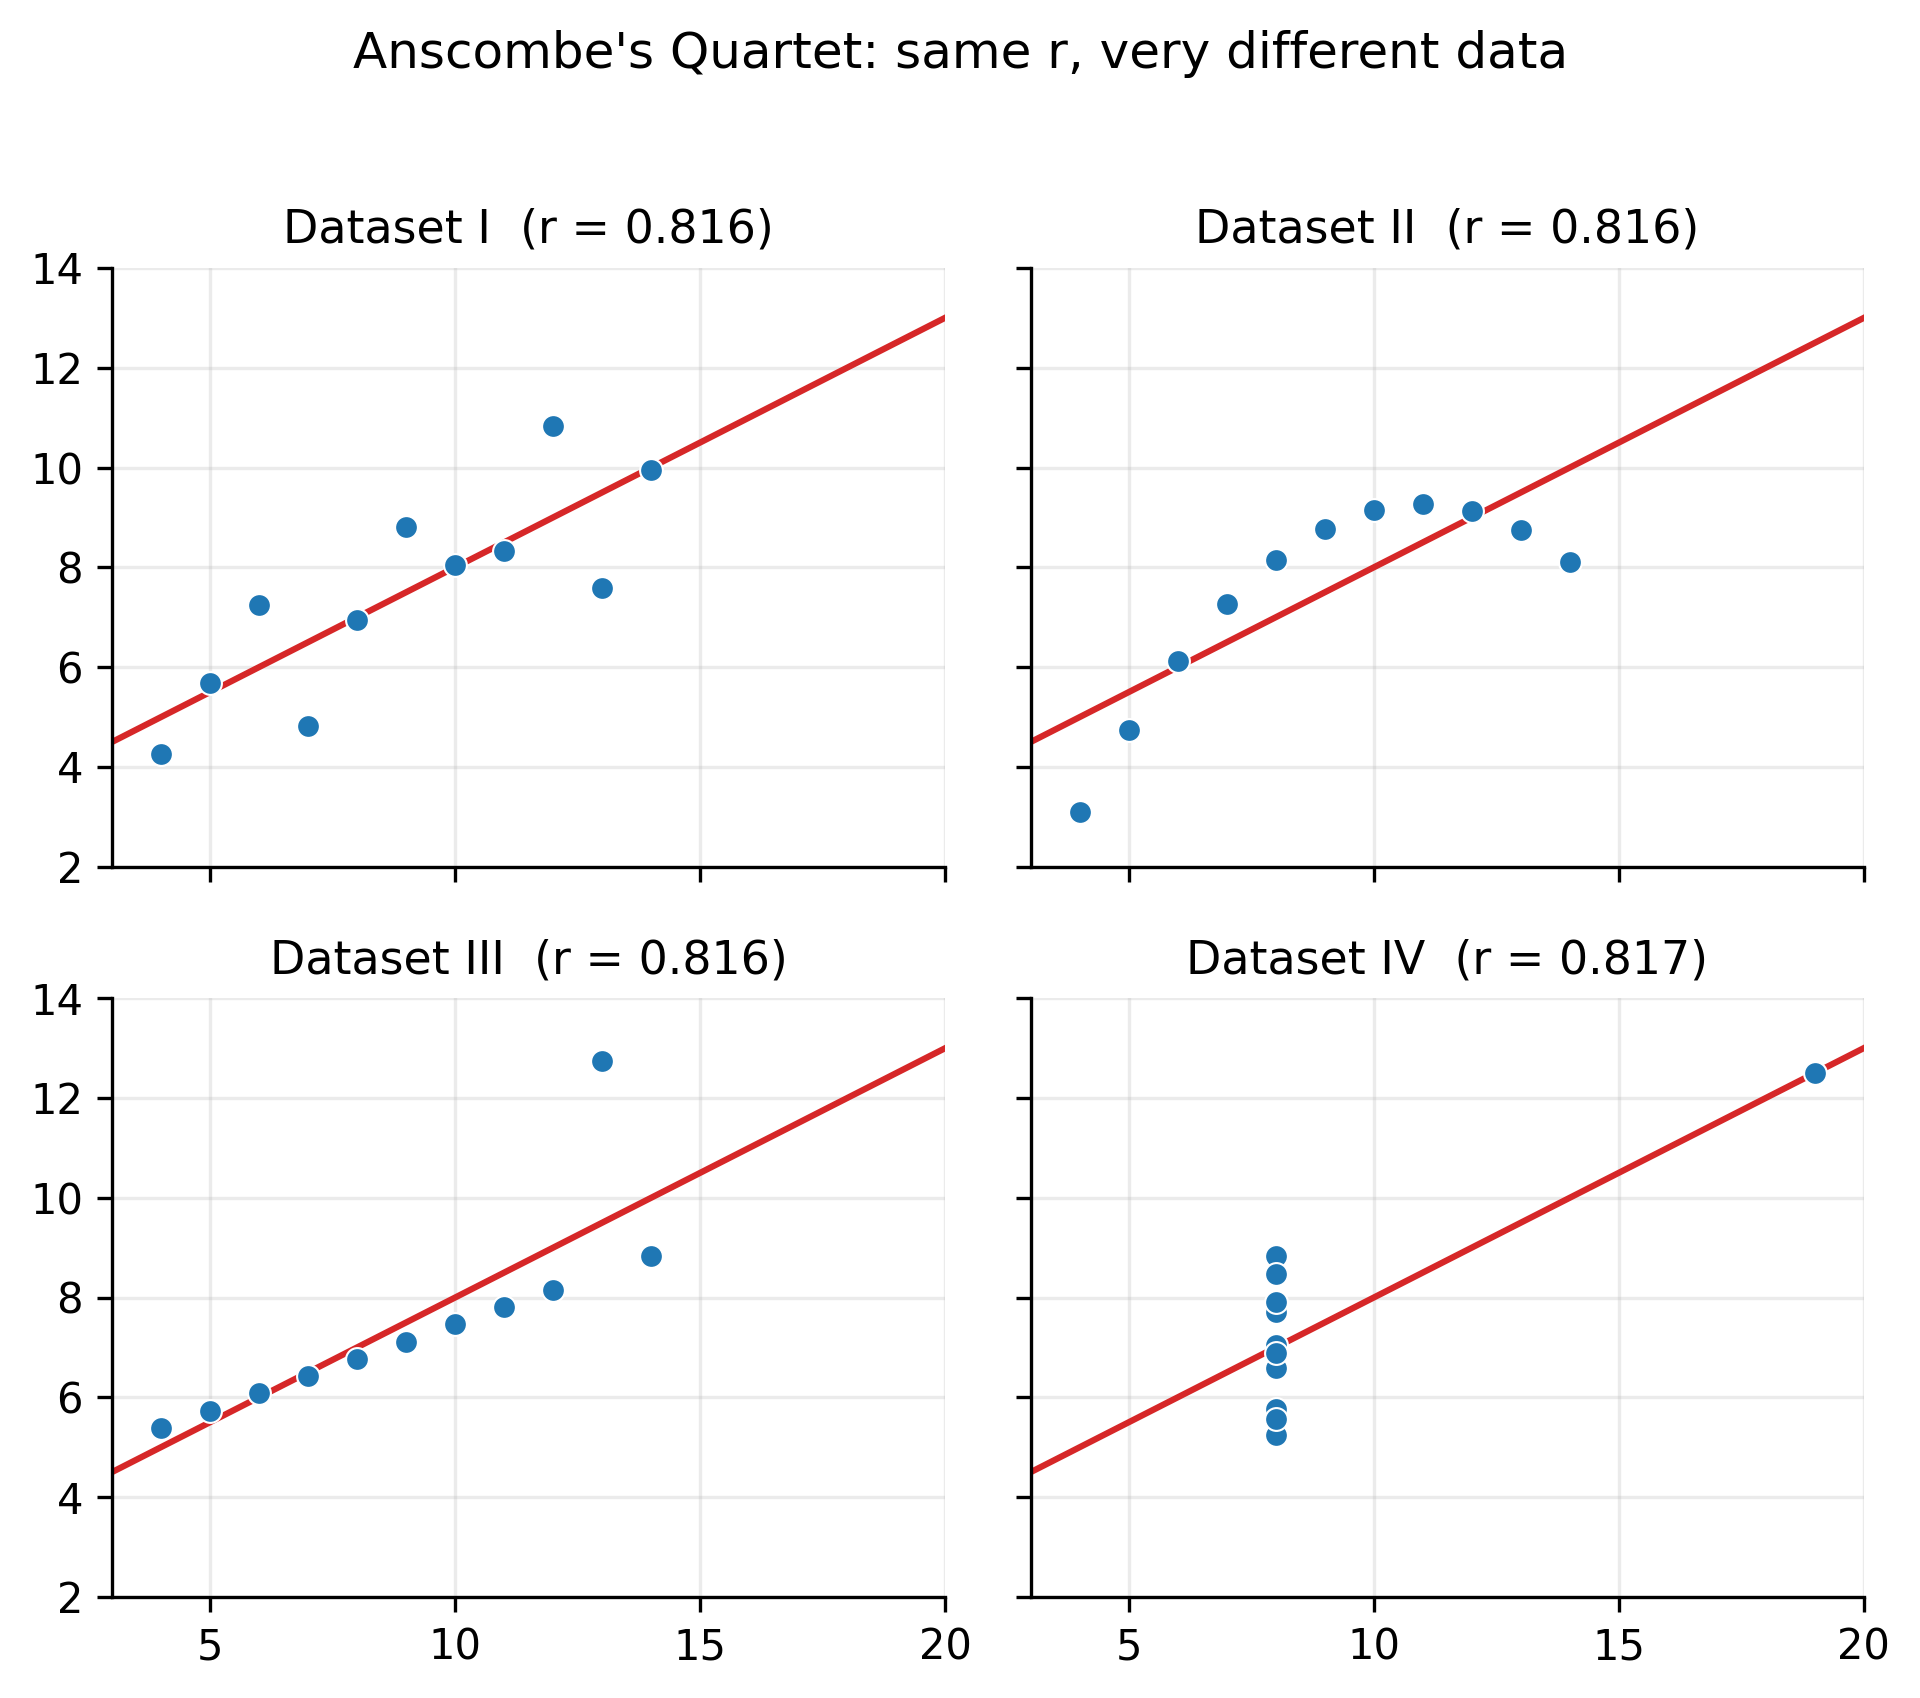
\includegraphics[width=0.85\linewidth]{figures/anscombe.png}
\caption{Anscombe's quartet: four datasets that share the same Pearson correlation ($r \approx 0.816$), means, variances, and regression line, but have radically different shapes. A single summary statistic is never a substitute for looking at the data.}
\label{fig:anscombe}
\end{figure}

\begin{figure}[h]
\centering
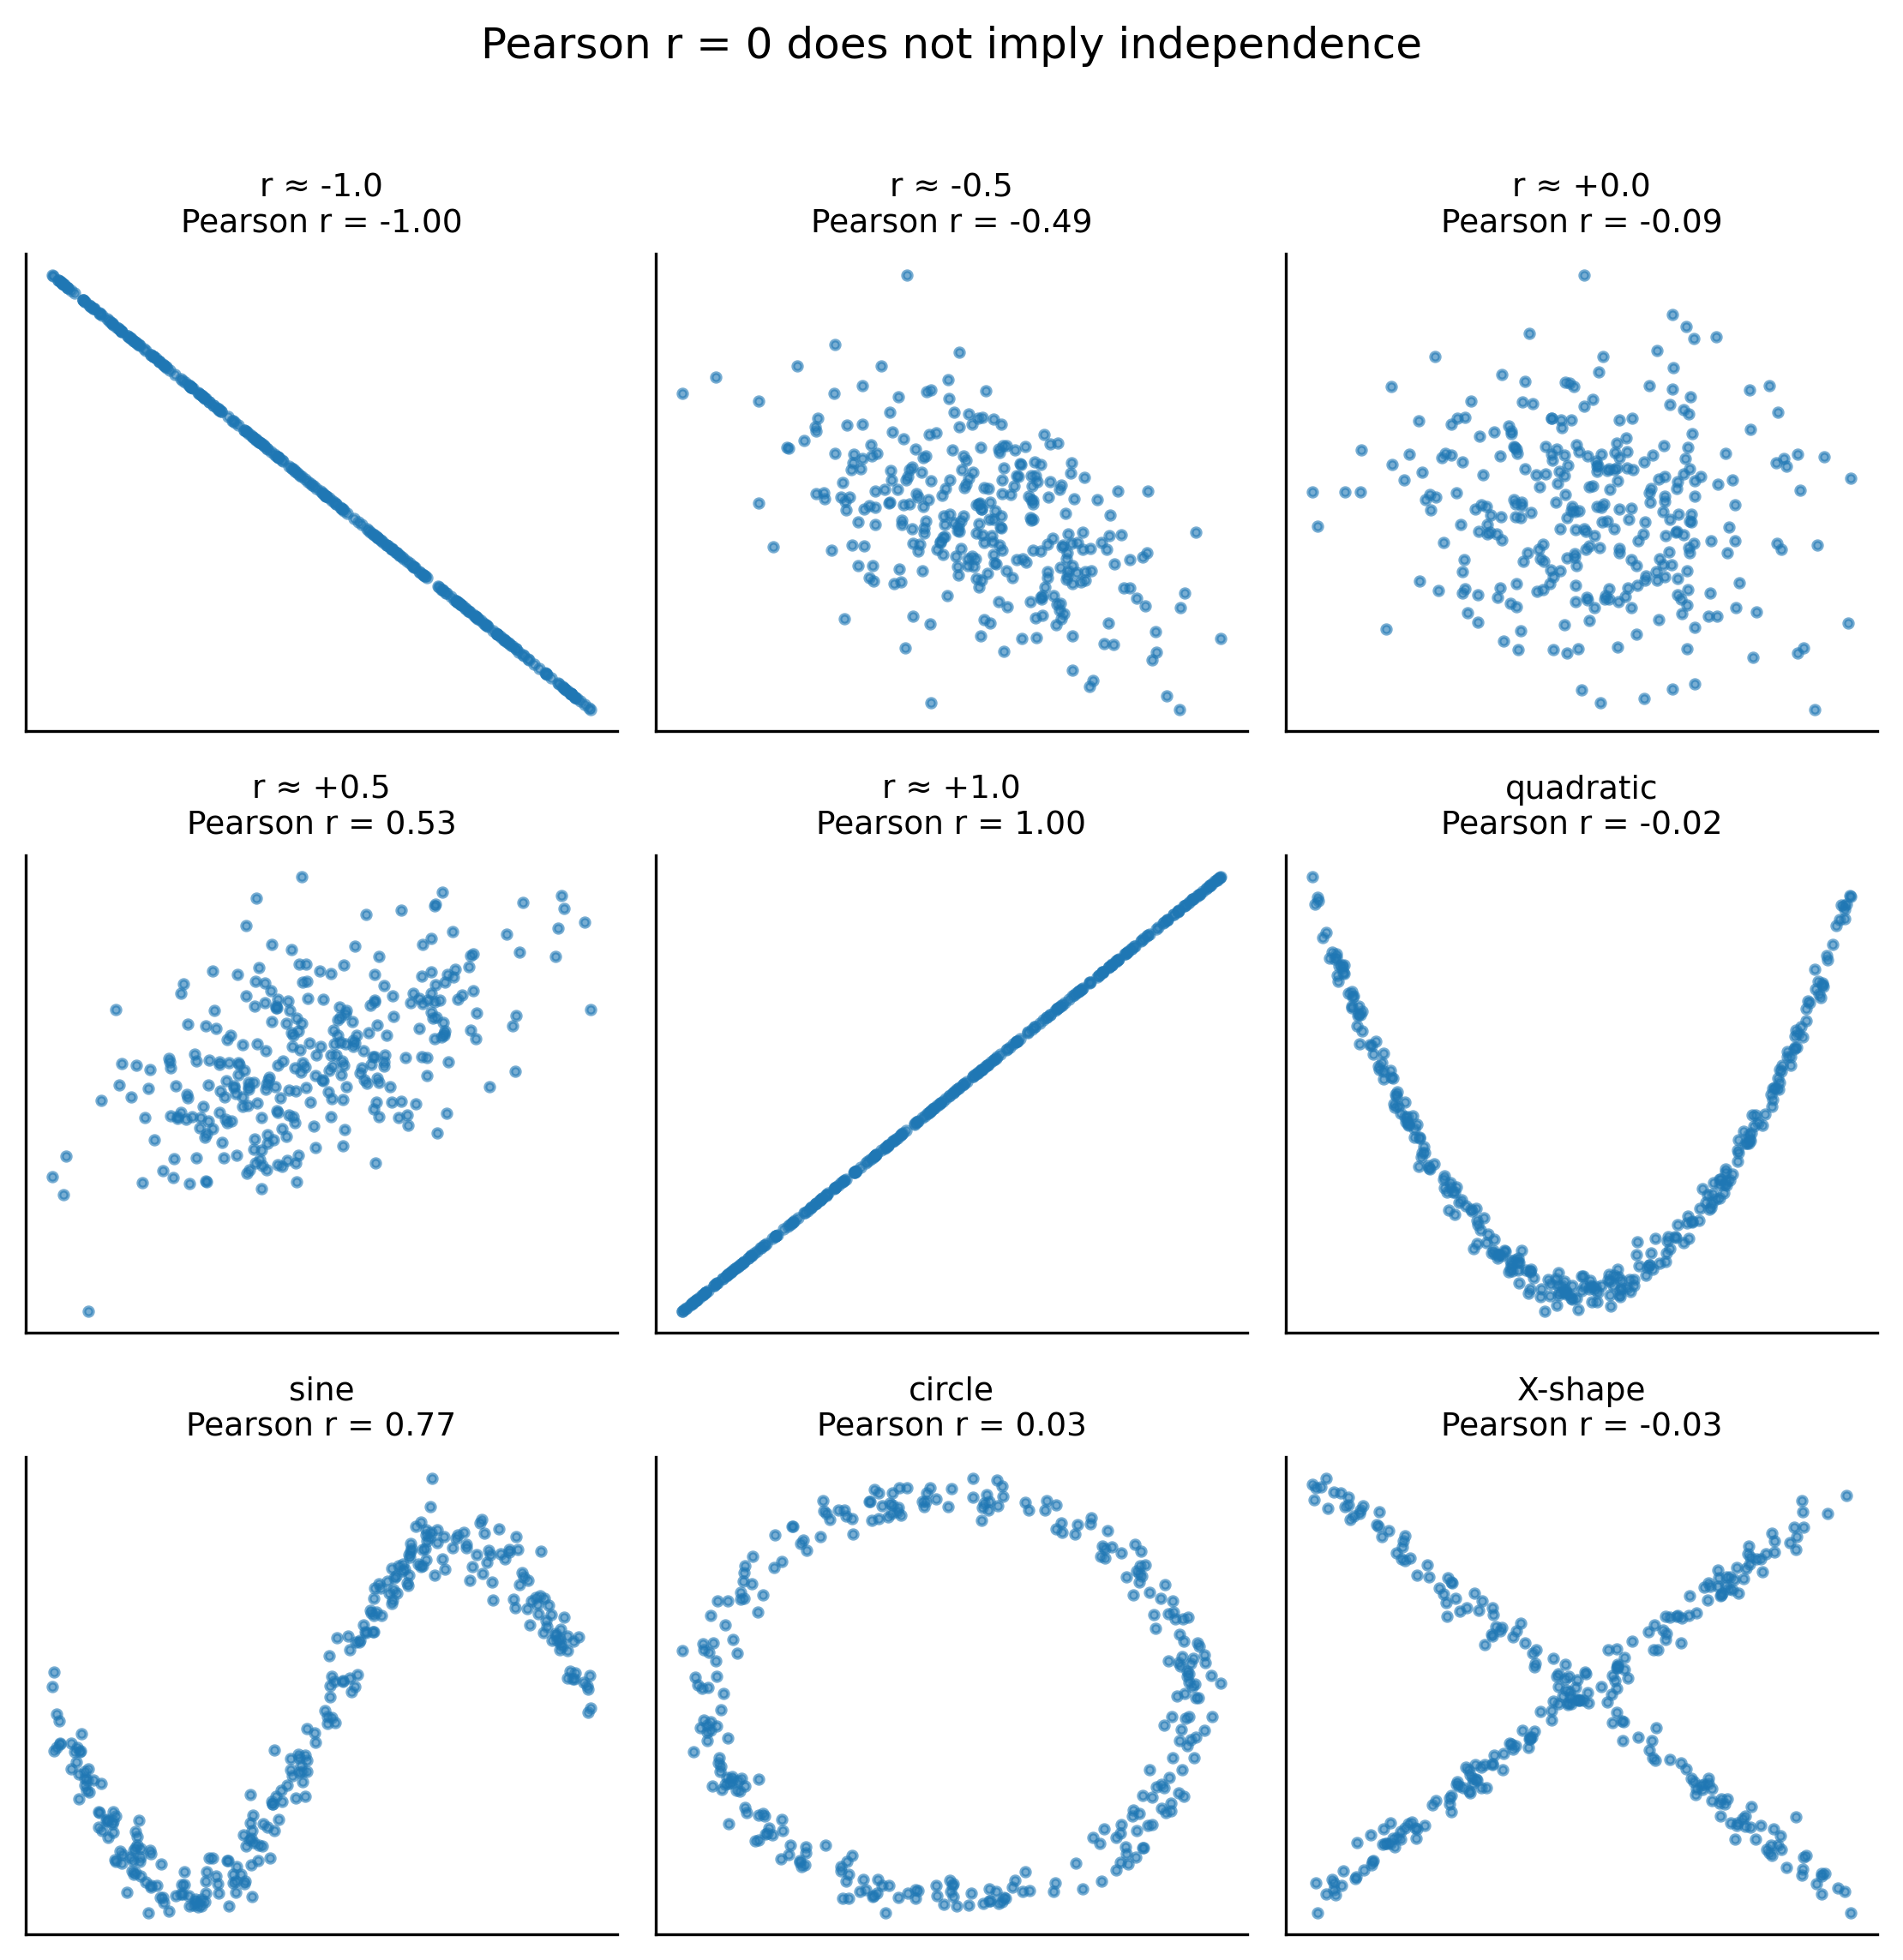
\includegraphics[width=0.85\linewidth]{figures/correlation_grid.png}
\caption{Pearson $r$ across nine joint distributions. The top row varies the underlying linear coefficient; the bottom row shows distinctly non-linear (but strongly dependent) patterns whose Pearson $r$ is near zero. $r = 0$ does \emph{not} imply independence.}
\label{fig:correlation-grid}
\end{figure}

\subsubsection{1.1 Definition}\label{11-definition}

For random variables \(X, Y\) with finite second moments, \[
\rho_{XY} = \frac{\mathrm{Cov}(X, Y)}{\sqrt{\mathrm{Var}(X)\,\mathrm{Var}(Y)}} = \frac{\mathbb{E}[(X - \mu_X)(Y - \mu_Y)]}{\sigma_X \sigma_Y}.
\]

The sample analogue: \[
r = \frac{\sum_{i=1}^{n} (x_i - \bar{x})(y_i - \bar{y})}{\sqrt{\sum_{i=1}^{n}(x_i - \bar{x})^2}\,\sqrt{\sum_{i=1}^{n}(y_i - \bar{y})^2}}.
\]

\subsubsection{1.2 Derivation and geometric
interpretation}\label{12-derivation-and-geometric-interpretation}

Centre the data: \(\tilde{x}_i = x_i - \bar{x}\),
\(\tilde{y}_i = y_i - \bar{y}\). Treat
\(\tilde{\mathbf{x}}, \tilde{\mathbf{y}}\) as vectors in
\(\mathbb{R}^n\). Then \[
r = \frac{\langle \tilde{\mathbf{x}}, \tilde{\mathbf{y}} \rangle}{\|\tilde{\mathbf{x}}\|\,\|\tilde{\mathbf{y}}\|} = \cos\theta,
\] where \(\theta\) is the angle between the two centred vectors. From
this:

\begin{itemize}
\tightlist
\item
  \(r = +1\) when \(\tilde{\mathbf{y}} = c \tilde{\mathbf{x}}\) for some
  \(c > 0\) (perfect positive linear relation).
\item
  \(r = -1\) when \(\tilde{\mathbf{y}} = c \tilde{\mathbf{x}}\) for some
  \(c < 0\) (perfect negative).
\item
  \(r = 0\) when the centred vectors are orthogonal.
\end{itemize}

The Cauchy--Schwarz inequality immediately gives \(|r| \leq 1\).
Equivalently, \(r\) is the slope of the \textbf{standardised} OLS
regression of \(y\) on \(x\): if \(z_x = (x - \bar{x})/s_x\) and
similarly \(z_y\), the OLS estimate of \(\beta\) in
\(z_y = \beta z_x + \varepsilon\) is exactly \(r\).

\subsubsection{1.3 Inference}\label{13-inference}

Under bivariate normality, the studentised statistic \[
t = r \sqrt{\frac{n - 2}{1 - r^2}}
\] is \(t\)-distributed with \(n - 2\) degrees of freedom under
\(H_0: \rho = 0\). \textbf{Fisher\textquotesingle s
\(z\)-transformation}: \[
z = \frac{1}{2} \ln \left( \frac{1 + r}{1 - r} \right) = \operatorname{arctanh}(r)
\] yields an asymptotically normal statistic with mean
\(\operatorname{arctanh}(\rho)\) and variance \(\tfrac{1}{n - 3}\), used
to construct CIs and to compare two correlations from independent
samples. The variance-stabilising property follows from a Taylor
expansion: \(\mathrm{Var}(r) \approx (1 - \rho^2)^2 / n\), and the
derivative \(z'(r) = 1/(1 - r^2)\) exactly cancels the factor.

\subsubsection{1.4 Properties}\label{14-properties}

\begin{itemize}
\tightlist
\item
  \textbf{Symmetry}: \(r(X, Y) = r(Y, X)\).
\item
  \textbf{Affine invariance}:
  \(r(aX + b, cY + d) = \mathrm{sign}(ac) \cdot r(X, Y)\) for
  \(a, c \neq 0\).
\item
  \textbf{Not monotonically invariant}: \(r(X, Y) \neq r(\log X, Y)\) in
  general.
\item
  \textbf{Bound on quadrant probability}: \(r = 0\) does \emph{not}
  imply independence.
\end{itemize}

\subsubsection{1.5 The canonical
counterexample}\label{15-the-canonical-counterexample}

Let \(X \sim \mathcal{U}(-1, 1)\) and \(Y = X^2\). Then
\(\mathbb{E}[X] = 0\), \(\mathbb{E}[XY] = \mathbb{E}[X^3] = 0\), so
\(\mathrm{Cov}(X, Y) = 0\) and \(r = 0\) --- yet \(Y\) is
\emph{deterministic} in \(X\). Pearson\textquotesingle s \(r\) is blind
to non-linear (especially symmetric) dependence. This single example
motivates the entirety of Parts II and III.

\subsubsection{1.6 Pitfalls}\label{16-pitfalls}

\begin{itemize}
\tightlist
\item
  \textbf{Outliers dominate}: squared deviations enter both numerator
  and denominator; a single high-leverage point can swing \(r\) from
  near 0 to near 1 or vice versa.
\item
  \textbf{Non-linearity is invisible}: always plot the data.
\item
  \textbf{Heteroscedasticity} does not bias \(r\) as a \emph{point}
  estimate but invalidates the \(t\)-test.
\item
  \textbf{Range restriction} attenuates \(r\): subsetting on \(X\)
  mechanically pulls \(r\) toward zero (the "restricted range" problem
  familiar in psychometrics).
\item
  \textbf{Anscombe\textquotesingle s quartet and the Datasaurus dozen}
  construct datasets with identical \(r\) but radically different
  scatter plots --- a permanent reminder that one number is never
  sufficient.
\end{itemize}

\subsubsection{1.7 Code}\label{17-code}

\begin{lstlisting}[language=Python]
import numpy as np
from scipy import stats

rng = np.random.default_rng(0)
n = 500
x = rng.normal(size=n)
y = 0.7 * x + 0.3 * rng.normal(size=n)

r, p = stats.pearsonr(x, y)
print(f"r = {r:.3f}, p = {p:.3g}")

# Fisher z confidence interval
z = np.arctanh(r)
se = 1.0 / np.sqrt(n - 3)
lo, hi = np.tanh(z - 1.96 * se), np.tanh(z + 1.96 * se)
print(f"95% CI: [{lo:.3f}, {hi:.3f}]")
\end{lstlisting}

\subsubsection{1.8 Worked tiny example}\label{18-worked-tiny-example}

Five points: \((1, 2), (2, 4), (3, 5), (4, 4), (5, 6)\).

\begin{itemize}
\tightlist
\item
  \(\bar{x} = 3\), \(\bar{y} = 4.2\).
\item
  \(\sum (x_i - \bar{x})(y_i - \bar{y}) = (-2)(-2.2) + (-1)(-0.2) + 0 \cdot 0.8 + 1 \cdot (-0.2) + 2 \cdot 1.8 = 4.4 + 0.2 + 0 - 0.2 + 3.6 = 8\).
\item
  \(\sum (x_i - \bar{x})^2 = 4 + 1 + 0 + 1 + 4 = 10\).
\item
  \(\sum (y_i - \bar{y})^2 = 4.84 + 0.04 + 0.64 + 0.04 + 3.24 = 8.8\).
\item
  \(r = 8 / \sqrt{10 \cdot 8.8} = 8 / \sqrt{88} \approx 0.853\).
\end{itemize}

\subsubsection{1.9 When to use / when
not}\label{19-when-to-use--when-not}

\textbf{Use} when data are continuous, the relationship is approximately
linear, outliers are absent, and you want a quick interpretable scalar.
\textbf{Avoid} for ordinal, ranked, heavy-tailed, or visibly non-linear
data; when you care about \emph{any} dependence rather than specifically
linear dependence.

\subsubsection{1.10 Cross-references}\label{110-cross-references}

For monotonic but non-linear relationships use
\hyperref[2-spearmans-rank-correlation-rho]{Spearman} or
\hyperref[3-kendalls-tau]{Kendall}. For any-shape dependence use
\hyperref[13-distance-correlation-dcor]{dCor},
\hyperref[16-hilbertschmidt-independence-criterion-hsic]{HSIC}, or
\hyperref[8-mutual-information-mi]{MI}.

\begin{center}\rule{0.5\linewidth}{0.5pt}\end{center}

\subsection{\texorpdfstring{2. Spearman\textquotesingle s Rank
Correlation
\(\rho\)}{2. Spearman\textquotesingle s Rank Correlation \textbackslash rho}}\label{2-spearmans-rank-correlation-rho}

\begin{figure}[h]
\centering
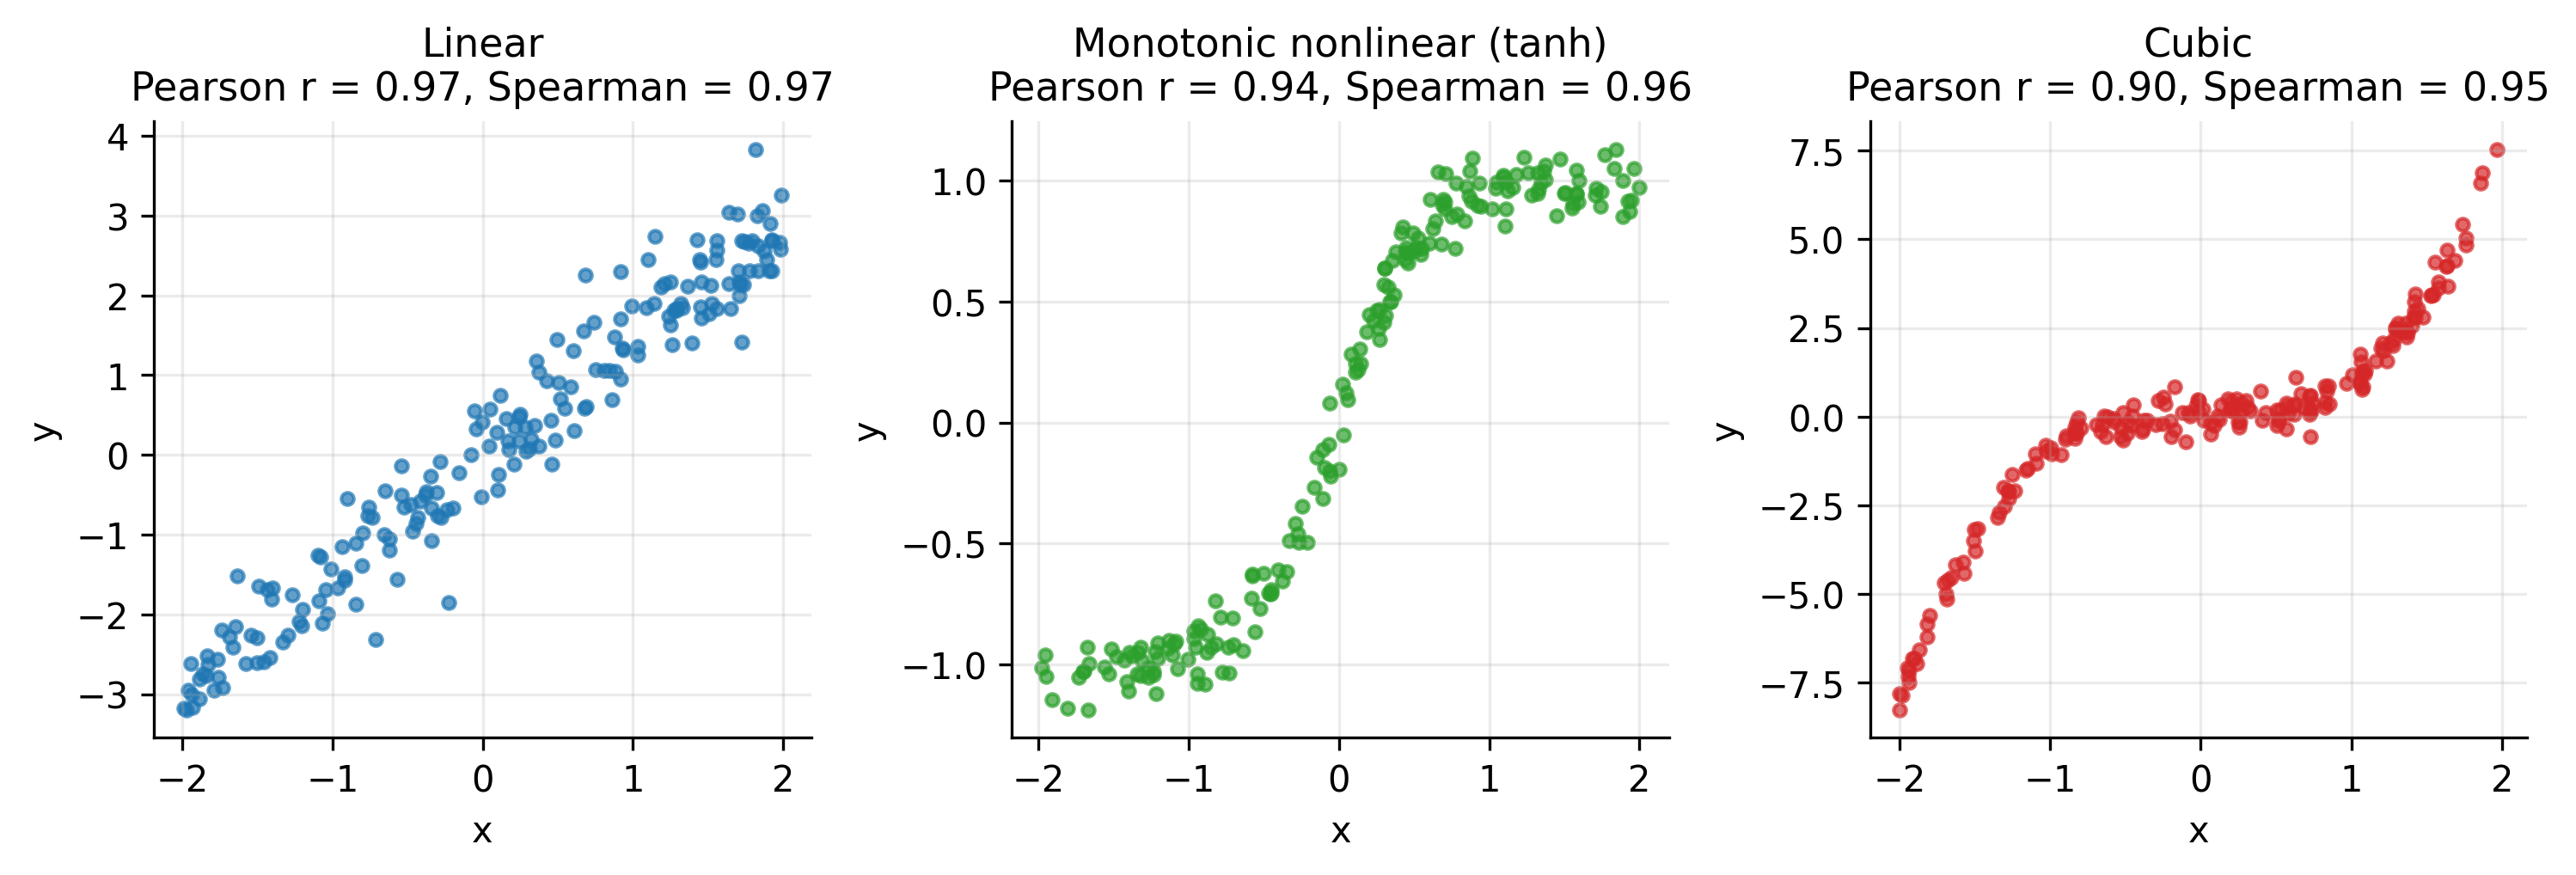
\includegraphics[width=0.95\linewidth]{figures/pearson_vs_rank.png}
\caption{Pearson vs.\ Spearman on three relationships. Left: linear data, both high. Middle: a monotonic squashing $y = \tanh(2x)$ where Spearman stays at $1$ while Pearson drops. Right: $y = x^3$, where Spearman is $\approx 1$ but Pearson is markedly lower. Spearman captures monotonicity; Pearson captures linearity.}
\label{fig:pearson-vs-rank}
\end{figure}

\subsubsection{2.1 Definition}\label{21-definition}

Replace observations by their ranks and apply Pearson. Let
\(R_i = \mathrm{rank}(x_i)\) and \(Q_i = \mathrm{rank}(y_i)\), both in
\(\{1, \dots, n\}\) (ties broken by averaging). Then \[
\rho_S = \mathrm{Pearson}(R, Q).
\] With \emph{no ties}, the convenient simplification (derivable from
the fact that \(\sum R_i = n(n+1)/2\) and
\(\sum R_i^2 = n(n+1)(2n+1)/6\)) is \[
\rho_S = 1 - \frac{6 \sum_{i=1}^{n} d_i^2}{n(n^2 - 1)}, \quad d_i = R_i - Q_i.
\]

\subsubsection{2.2 Derivation of the shortcut
formula}\label{22-derivation-of-the-shortcut-formula}

When ranks are a permutation of \(\{1, \dots, n\}\), the mean rank is
\(\bar{R} = (n+1)/2\) and \(\sum_i (R_i - \bar{R})^2 = n(n^2 - 1)/12\).
Substituting into Pearson\textquotesingle s formula: \[
\rho_S = \frac{\sum_i (R_i - \bar{R})(Q_i - \bar{R})}{n(n^2 - 1)/12}.
\] Expanding
\(\sum_i (R_i - Q_i)^2 = \sum_i (R_i - \bar{R})^2 + \sum_i (Q_i - \bar{R})^2 - 2 \sum_i (R_i - \bar{R})(Q_i - \bar{R})\)
and solving: \[
\sum_i (R_i - \bar{R})(Q_i - \bar{R}) = \frac{n(n^2 - 1)}{12} - \frac{1}{2}\sum_i d_i^2.
\] Divide by \(n(n^2 - 1)/12\) and simplify to obtain the famous form
\(1 - 6\sum d_i^2 / (n(n^2 - 1))\).

\subsubsection{2.3 Intuition}\label{23-intuition}

\(\rho_S\) measures the strength of the \textbf{monotonic} relationship:
any strictly increasing transformation \(X \mapsto g(X)\) leaves
\(\rho_S\) unchanged because \(g\) preserves ranks. It is therefore
\emph{scale-free} and \emph{outlier-robust} --- replacing the largest
observation by an arbitrarily larger number changes only its rank, not
the calculation.

\subsubsection{2.4 Relationship to
Pearson}\label{24-relationship-to-pearson}

For jointly normal \((X, Y)\) with population correlation \(\rho\), \[
\rho_S = \frac{6}{\pi} \arcsin\!\left(\frac{\rho}{2}\right) \approx 0.92\,\rho \text{ for moderate } |\rho|.
\] For monotonic but non-linear relations (e.g. \(Y = \tanh(X)\) +
noise), Spearman exceeds Pearson --- sometimes substantially. This gap
is a useful diagnostic: a large \(\rho_S - r\) signals non-linear
monotonicity.

\subsubsection{2.5 Inference}\label{25-inference}

For \(n \gtrsim 10\), \[
t_S = \rho_S \sqrt{\frac{n - 2}{1 - \rho_S^2}} \overset{H_0}{\approx} t_{n-2}.
\] Exact tables exist for small \(n\) (Olds 1938); permutation tests are
exact and the default for heavy ties.

\subsubsection{2.6 Tie handling}\label{26-tie-handling}

With ties, the simple shortcut formula is biased.
SciPy\textquotesingle s \texttt{spearmanr} applies the tie-corrected
formula automatically. When more than \textasciitilde25\% of values are
tied, consider Kendall\textquotesingle s \(\tau_b\) instead --- it
handles ties more gracefully.

\subsubsection{2.7 Code}\label{27-code}

\begin{lstlisting}[language=Python]
from scipy import stats
import numpy as np

rng = np.random.default_rng(0)
x = rng.normal(size=200)
y = np.tanh(2 * x) + 0.1 * rng.normal(size=200)

r_pearson, _ = stats.pearsonr(x, y)
rho_spearman, _ = stats.spearmanr(x, y)
print(f"Pearson r  = {r_pearson:.3f}")
print(f"Spearman rho = {rho_spearman:.3f}")
# Spearman is materially larger because the relationship is monotonic-NL
\end{lstlisting}

\subsubsection{2.8 Worked tiny example}\label{28-worked-tiny-example}

Same five points \((1, 2), (2, 4), (3, 5), (4, 4), (5, 6)\).

Ranks of \(x\): \(1, 2, 3, 4, 5\). Ranks of \(y\): \(1, 2.5, 4, 2.5, 5\)
(the two 4\textquotesingle s tied at midrank 2.5). Without tie
correction: \(d = (0, -0.5, -1, 1.5, 0)\),
\(\sum d^2 = 0 + 0.25 + 1 + 2.25 + 0 = 3.5\).
\(\rho_S \approx 1 - 6(3.5)/(5 \cdot 24) = 1 - 21/120 = 0.825\).

\subsubsection{2.9 Pitfalls}\label{29-pitfalls}

\begin{itemize}
\tightlist
\item
  \textbf{Ties} require correction; use \texttt{spearmanr} not the
  shortcut.
\item
  \textbf{Discrete or coarse variables} lose resolution under ranking.
\item
  \textbf{Monotonicity is not all you want}: U-shaped or sinusoidal
  relationships have \(\rho_S \approx 0\).
\end{itemize}

\subsubsection{2.10 When to use / when
not}\label{210-when-to-use--when-not}

\textbf{Use} for ordinal data; continuous data with outliers or visibly
non-linear-but-monotonic shape; any robust-correlation slot in EDA.
\textbf{Avoid} when the relationship is non-monotonic --- switch to
\hyperref[13-distance-correlation-dcor]{dCor} or
\hyperref[17-chatterjees-rank-correlation-xi]{Chatterjee\textquotesingle s
\(\xi\)}.

\begin{center}\rule{0.5\linewidth}{0.5pt}\end{center}

\subsection{\texorpdfstring{3. Kendall\textquotesingle s
\(\tau\)}{3. Kendall\textquotesingle s \textbackslash tau}}\label{3-kendalls-tau}

\subsubsection{3.1 Definition}\label{31-definition}

A pair of observations \((x_i, y_i), (x_j, y_j)\) is \textbf{concordant}
if \((x_i - x_j)(y_i - y_j) > 0\), \textbf{discordant} if negative,
\textbf{tied} otherwise. Out of \(\binom{n}{2}\) pairs, let \(C\) be the
number of concordant and \(D\) the number of discordant: \[
\tau_a = \frac{C - D}{\binom{n}{2}}.
\] The tie-corrected \(\tau_b\): \[
\tau_b = \frac{C - D}{\sqrt{(C + D + T_x)(C + D + T_y)}},
\] where \(T_x, T_y\) count pairs tied on \(X\) or \(Y\) but not both.
\(\tau_c\) is a further variant for non-square contingency tables.

\subsubsection{3.2 Probabilistic
interpretation}\label{32-probabilistic-interpretation}

Define
\(\tau = P\{(X_1 - X_2)(Y_1 - Y_2) > 0\} - P\{(X_1 - X_2)(Y_1 - Y_2) < 0\}\)
for independent copies \((X_1, Y_1), (X_2, Y_2)\). The sample \(\tau_a\)
is an unbiased U-statistic for this functional with kernel
\(h((x_i, y_i), (x_j, y_j)) = \mathrm{sgn}(x_i - x_j) \mathrm{sgn}(y_i - y_j)\).

Equivalently, \(\tau \in [-1, 1]\) where the probability that a randomly
chosen pair is concordant equals \((1 + \tau)/2\). This
\emph{probabilistic} interpretation is the cleanest in the entire
correlation literature.

\subsubsection{3.3 Computation}\label{33-computation}

Naively \(O(n^2)\), but Knight\textquotesingle s (1966) merge-sort-based
algorithm achieves \(O(n \log n)\) and is the implementation in
\texttt{scipy.stats.kendalltau}. Idea: sort by \(x\); then \(D\) =
number of inversions in the \(y\)-sequence, which merge sort counts as a
by-product.

\subsubsection{3.4 Relationship to Spearman and
Pearson}\label{34-relationship-to-spearman-and-pearson}

Under bivariate normality: \[
\tau = \frac{2}{\pi} \arcsin(\rho), \qquad \rho_S = \frac{6}{\pi} \arcsin\!\left(\frac{\rho}{2}\right).
\] Empirically \(\rho_S / \tau \approx 1.5\) across most of the range,
and \(\tau\) is roughly \(\tfrac{2}{3} \rho_S\).

\subsubsection{3.5 Inference}\label{35-inference}

Under \(H_0\) of independence, \(\mathbb{E}[\tau] = 0\) and
\(\mathrm{Var}(\tau) = 2(2n + 5)/(9n(n-1))\);
\(\sqrt{n}\,\tau \to_d \mathcal{N}(0, 4/9 \cdot \mathrm{const})\) ---
more precisely
\(\sqrt{(9n(n-1))/(2(2n+5))} \cdot \tau \to_d \mathcal{N}(0, 1)\). Exact
null distributions are tabulated for \(n < 50\).

\subsubsection{3.6 Code}\label{36-code}

\begin{lstlisting}[language=Python]
from scipy import stats
import numpy as np

rng = np.random.default_rng(0)
x = rng.normal(size=100)
y = x + rng.normal(size=100) * 0.5

tau, p = stats.kendalltau(x, y)
print(f"Kendall tau_b = {tau:.3f}, p = {p:.3g}")
\end{lstlisting}

\subsubsection{3.7 Worked tiny example}\label{37-worked-tiny-example}

Points \((1, 2), (2, 4), (3, 5), (4, 4), (5, 6)\). The
\(\binom{5}{2} = 10\) pairs and their concordance:

{\def\LTcaptype{none} % do not increment counter
\begin{longtable}[]{@{}llll@{}}
\toprule\noalign{}
pair & \(\Delta x\) & \(\Delta y\) & concordant? \\
\midrule\noalign{}
\endhead
\bottomrule\noalign{}
\endlastfoot
(1,2)-(2,4) & + & + & C \\
(1,2)-(3,5) & + & + & C \\
(1,2)-(4,4) & + & + & C \\
(1,2)-(5,6) & + & + & C \\
(2,4)-(3,5) & + & + & C \\
(2,4)-(4,4) & + & 0 & tied on \(y\) \\
(2,4)-(5,6) & + & + & C \\
(3,5)-(4,4) & + & − & D \\
(3,5)-(5,6) & + & + & C \\
(4,4)-(5,6) & + & + & C \\
\end{longtable}
}

\(C = 8\), \(D = 1\), one \(y\)-tie.
\(\tau_b = (8 - 1)/\sqrt{(8 + 1 + 0)(8 + 1 + 1)} = 7/\sqrt{90} \approx 0.738\).

\subsubsection{3.8 Pitfalls and
trade-offs}\label{38-pitfalls-and-trade-offs}

\begin{itemize}
\tightlist
\item
  \textbf{More robust to outliers than Spearman}: Spearman still uses
  squared rank differences; Kendall counts signs.
\item
  \textbf{Lower power than Spearman for smooth alternatives} in some
  regimes; more reliable on weak or noisy signals.
\item
  \textbf{Tie correction is nontrivial} ---
  \texttt{scipy.stats.kendalltau} returns \(\tau_b\) by default; report
  which variant.
\end{itemize}

\subsubsection{3.9 When to use / when
not}\label{39-when-to-use--when-not}

\textbf{Use} for ordinal data with ties, small samples (exact
distributions available), and any time you want a probabilistic
interpretation ("randomly chosen pair concordant with probability
\((1 + \tau)/2\)"). \textbf{Avoid} for very large \(n\) where the
\(O(n \log n)\) cost beats the \(O(n)\) Pearson by a constant factor
that no longer matters.

\begin{center}\rule{0.5\linewidth}{0.5pt}\end{center}

\subsection{\texorpdfstring{4. Point-Biserial Correlation
\(r_{pb}\)}{4. Point-Biserial Correlation r\_\{pb\}}}\label{4-point-biserial-correlation-r_pb}

\subsubsection{4.1 Definition and equivalence to
Pearson}\label{41-definition-and-equivalence-to-pearson}

A degenerate case of Pearson when one variable is dichotomous (coded
0/1). Let \(Y\) be continuous and \(X \in \{0, 1\}\) with group sizes
\(n_1, n_0\), group means \(\bar{y}_1, \bar{y}_0\), and pooled SD
\(s_y\): \[
r_{pb} = \frac{\bar{y}_1 - \bar{y}_0}{s_y}\sqrt{\frac{n_1 n_0}{n^2}}.
\] This is \textbf{identical} to applying Pearson\textquotesingle s
formula directly to the 0/1 coded variable.

\subsubsection{4.2 Derivation}\label{42-derivation}

With \(X \in \{0, 1\}\) coded, \(\bar{x} = n_1 / n\),
\(\sum_i (x_i - \bar{x})^2 = n_1 (n_0/n)^2 + n_0 (n_1/n)^2 = n_1 n_0 / n\),
so \(s_x = \sqrt{n_1 n_0 / (n(n-1))}\). The numerator
\(\sum_i (x_i - \bar{x})(y_i - \bar{y}) = (n_1 n_0 / n)(\bar{y}_1 - \bar{y}_0)\).
Substituting and simplifying gives the formula above.

\subsubsection{\texorpdfstring{4.3 Relation to the two-sample
\(t\)-test}{4.3 Relation to the two-sample t-test}}\label{43-relation-to-the-two-sample-t-test}

\(r_{pb}\) is monotonically equivalent to the independent-samples \(t\):
\[
t = r_{pb} \sqrt{\frac{n - 2}{1 - r_{pb}^2}}, \quad \mathrm{df} = n - 2.
\] Thus the \(p\)-value of \(r_{pb}\) from \texttt{pointbiserialr} is
identical (up to floating-point precision) to that of
\texttt{ttest\_ind} on the two groups.

\subsubsection{4.4 Point-biserial versus
biserial}\label{44-point-biserial-versus-biserial}

\begin{itemize}
\tightlist
\item
  \textbf{Point-biserial} assumes \(X\) is \emph{intrinsically} binary
  (sex, treatment/control).
\item
  \textbf{Biserial} (\(r_b\)) assumes \(X\) is a coarse-grained version
  of a latent continuous normal --- for example a pass/fail derived from
  an underlying score. It rescales: \[
  r_b = r_{pb} \cdot \frac{\sqrt{pq}}{\varphi(z_p)},
  \] where \(p = n_1/n\), \(q = 1-p\), \(z_p = \Phi^{-1}(p)\), and
  \(\varphi\) is the standard normal PDF. \(r_b\) is always
  \(\geq |r_{pb}|\) in magnitude.
\end{itemize}

Use \(r_{pb}\) when the binary variable is genuinely binary; use \(r_b\)
only if you have substantive reason to believe a latent continuous
variable was thresholded.

\subsubsection{\texorpdfstring{4.5 Bound on
\(|r_{pb}|\)}{4.5 Bound on \textbar r\_\{pb\}\textbar{}}}\label{45-bound-on-r_pb}

\(|r_{pb}| \leq \sqrt{n_1 n_0 / n^2}\), which is at most \(1/2\) when
\(n_1 = n_0\) and tends to zero as groups become imbalanced. A 99/1
split caps \(|r_{pb}|\) at \(\sqrt{0.99 \cdot 0.01} \approx 0.099\) even
when the means are wildly different --- a major reason to also report
effect sizes like Cohen\textquotesingle s \(d\).

\subsubsection{4.6 Code}\label{46-code}

\begin{lstlisting}[language=Python]
from scipy import stats
import numpy as np

rng = np.random.default_rng(0)
group = rng.integers(0, 2, size=200)
score = group * 0.8 + rng.normal(size=200)

r_pb, p = stats.pointbiserialr(group, score)
print(f"r_pb = {r_pb:.3f}, p = {p:.3g}")
\end{lstlisting}

\subsubsection{4.7 When to use / when
not}\label{47-when-to-use--when-not}

\textbf{Use} when correlating a continuous variable with a true binary
one (sex, churn, conversion) and you want a correlation-style effect
size alongside a \(t\)-test. \textbf{Avoid} when the binary variable is
a coarse-grained continuous one (use biserial), or when groups are
extremely imbalanced (interpret the cap on magnitude).

\begin{center}\rule{0.5\linewidth}{0.5pt}\end{center}

\subsection{\texorpdfstring{5. The Phi Coefficient
\(\phi\)}{5. The Phi Coefficient \textbackslash phi}}\label{5-the-phi-coefficient-phi}

\subsubsection{5.1 Definition}\label{51-definition}

For a \(2 \times 2\) contingency table

{\def\LTcaptype{none} % do not increment counter
\begin{longtable}[]{@{}lll@{}}
\toprule\noalign{}
& \(Y = 0\) & \(Y = 1\) \\
\midrule\noalign{}
\endhead
\bottomrule\noalign{}
\endlastfoot
\(X = 0\) & \(a\) & \(b\) \\
\(X = 1\) & \(c\) & \(d\) \\
\end{longtable}
}

\[
\phi = \frac{ad - bc}{\sqrt{(a+b)(c+d)(a+c)(b+d)}}.
\] This is exactly Pearson\textquotesingle s \(r\) applied to the 0/1
codings.

\subsubsection{\texorpdfstring{5.2 Relation to
\(\chi^2\)}{5.2 Relation to \textbackslash chi\^{}2}}\label{52-relation-to-chi2}

The Pearson chi-squared statistic for the \(2 \times 2\) table is \[
\chi^2 = \frac{n(ad - bc)^2}{(a+b)(c+d)(a+c)(b+d)},
\] hence \(\phi^2 = \chi^2 / n\). This links the \emph{test}
(chi-squared) and the \emph{effect size} (phi) into one calculation.

\subsubsection{5.3 Bounds and marginal-dependence
pathology}\label{53-bounds-and-marginal-dependence-pathology}

\(\phi \in [-1, 1]\) \emph{in principle}, but the maximum attainable
depends on the marginals. If \(a + b \neq a + c\) (i.e., row and column
marginals are unequal), \(|\phi|_{\max} < 1\). The \textbf{maximum} is
\[
\phi_{\max} = \sqrt{\frac{p_{1+} q_{+1}}{q_{1+} p_{+1}}}
\] where \(p_{i+}, p_{+j}\) are marginal probabilities --- useful to
know when comparing \(\phi\) across tables with different marginals.

\subsubsection{5.4 Versus the odds
ratio}\label{54-versus-the-odds-ratio}

For \(2 \times 2\) tables many epidemiologists prefer the odds ratio
\(\mathrm{OR} = (ad)/(bc)\), which is invariant to whether the data come
from prospective, retrospective, or cross-sectional sampling and is the
natural parameter in logistic regression. \(\phi\) is symmetric and
bounded but lacks \(\mathrm{OR}\)\textquotesingle s sampling invariance.

A useful rule: report \textbf{both} for \(2 \times 2\) analyses ---
\(\phi\) as effect size, \(\mathrm{OR}\) for design-invariant inference.

\subsubsection{5.5 Code}\label{55-code}

\begin{lstlisting}[language=Python]
import numpy as np
from scipy.stats import chi2_contingency

# Confusion-style table
table = np.array([[40, 10],
                  [ 5, 45]])
chi2, p, dof, expected = chi2_contingency(table, correction=False)
n = table.sum()
phi = np.sqrt(chi2 / n) * np.sign(table[0, 0] * table[1, 1] - table[0, 1] * table[1, 0])
print(f"phi = {phi:.3f}, chi2 = {chi2:.2f}, p = {p:.3g}")
\end{lstlisting}

\subsubsection{5.6 When to use}\label{56-when-to-use}

A/B test responses, two-class agreement, any binary-binary association.
For sparse cells (any expected count \textless{} 5), prefer
Fisher\textquotesingle s exact test for the \(p\)-value.

\begin{center}\rule{0.5\linewidth}{0.5pt}\end{center}

\subsection{\texorpdfstring{6. Cramér\textquotesingle s
\(V\)}{6. Cramér\textquotesingle s V}}\label{6-cramuxe9rs-v}

\subsubsection{6.1 Definition}\label{61-definition}

For an \(r \times c\) contingency table with chi-squared statistic
\(\chi^2\) and total \(n\), \[
V = \sqrt{\frac{\chi^2 / n}{\min(r - 1, c - 1)}}.
\]

\subsubsection{6.2 Derivation of the
normalisation}\label{62-derivation-of-the-normalisation}

For any \(r \times c\) table, the maximum value of \(\chi^2\) is
\(n \cdot \min(r-1, c-1)\), attained when each row is concentrated in a
single column (or vice versa). Dividing \(\chi^2/n\) by this maximum
normalises \(V\) to \([0, 1]\).

\subsubsection{6.3 Properties}\label{63-properties}

\begin{itemize}
\tightlist
\item
  Always non-negative; no sign because categorical variables lack a
  natural ordering.
\item
  Reduces to \(|\phi|\) for \(2 \times 2\) tables.
\item
  Invariant under relabelling of categories (the partition into cells is
  what matters).
\end{itemize}

\subsubsection{6.4 Bias correction (Bergsma
2013)}\label{64-bias-correction-bergsma-2013}

For small \(n\) or sparse tables, \(V\) is upward biased. The
bias-corrected: \[
\tilde{V} = \sqrt{\max\!\left(0, \frac{\chi^2/n - (r-1)(c-1)/(n-1)}{\min(\tilde{r}-1, \tilde{c}-1)}\right)}, \quad \tilde{k} = k - \frac{(k-1)^2}{n-1}.
\] Strongly recommended when \(n\) is small or any cell count is below
\textasciitilde10.

\subsubsection{6.5 Code}\label{65-code}

\begin{lstlisting}[language=Python]
import numpy as np
from scipy.stats import chi2_contingency

def cramers_v(table, bias_correction=True):
    table = np.asarray(table)
    chi2, _, _, _ = chi2_contingency(table, correction=False)
    n = table.sum()
    r, c = table.shape
    phi2 = chi2 / n
    if bias_correction:
        phi2 = max(0, phi2 - (r - 1) * (c - 1) / (n - 1))
        r_tilde = r - (r - 1) ** 2 / (n - 1)
        c_tilde = c - (c - 1) ** 2 / (n - 1)
        return np.sqrt(phi2 / min(r_tilde - 1, c_tilde - 1))
    return np.sqrt(phi2 / min(r - 1, c - 1))

table = np.array([[50, 20, 10],
                  [10, 40, 50]])
print(f"V = {cramers_v(table, bias_correction=False):.3f}")
print(f"V (bias-corrected) = {cramers_v(table, bias_correction=True):.3f}")
\end{lstlisting}

\subsubsection{6.6 Pitfalls}\label{66-pitfalls}

\begin{itemize}
\tightlist
\item
  \textbf{High-cardinality categoricals} inflate \(\chi^2\) and
  therefore \(V\) --- bin or regularise (e.g. group low-frequency levels
  into "Other").
\item
  \textbf{Sparse cells} invalidate the \(\chi^2\) approximation for the
  \emph{test} (use Monte Carlo or exact); the point estimate \(V\)
  remains meaningful.
\item
  \(V\) does not tell you \emph{where} the association lives; pair with
  a mosaic plot or standardised residuals.
\end{itemize}

\subsubsection{6.7 When to use}\label{67-when-to-use}

Categorical--categorical EDA, feature screening with mixed types, mosaic
plot annotations. The natural Pearson analogue for fully categorical
data.

\begin{center}\rule{0.5\linewidth}{0.5pt}\end{center}

\subsection{7. Tetrachoric and Polychoric
Correlation}\label{7-tetrachoric-and-polychoric-correlation}

\subsubsection{7.1 The latent-normal
model}\label{71-the-latent-normal-model}

Assume the \emph{observed} categorical variables
\(X \in \{1, \dots, r\}\), \(Y \in \{1, \dots, c\}\) are coarse-grained
slices of underlying jointly normal continuous
\((X^\star, Y^\star) \sim \mathcal{N}_2(\mathbf{0}, \Sigma)\),
\(\Sigma = \begin{pmatrix} 1 & \rho \\ \rho & 1 \end{pmatrix}\), with
thresholds \(\tau_1^X < \dots < \tau_{r-1}^X\) and
\(\tau_1^Y < \dots < \tau_{c-1}^Y\) such that
\(X = k \iff \tau_{k-1}^X < X^\star \leq \tau_k^X\).

\begin{itemize}
\tightlist
\item
  \textbf{Tetrachoric} = polychoric with \(r = c = 2\).
\item
  \textbf{Polychoric} = the general ordinal case.
\end{itemize}

The parameter of interest is \(\rho\), the correlation between the
latent continuous variables.

\subsubsection{7.2 Why bother}\label{72-why-bother}

Pearson\textquotesingle s \(r\) on the ordinal codes is
\emph{attenuated}: categorising continuous variables throws away
information and biases the correlation toward zero. Dichotomising two
truly normal variables with \(\rho = 0.7\) at the medians yields
\(\phi \approx 0.49\). Tetrachoric/polychoric reverse-engineer the
latent correlation, recovering \(\rho\) close to the true value
\emph{if} the normality assumption holds.

\subsubsection{7.3 Estimation}\label{73-estimation}

Two methods in standard use:

\begin{itemize}
\tightlist
\item
  \textbf{Two-step}: estimate thresholds from marginal frequencies via
  inverse normal CDF; then maximise the bivariate-normal likelihood over
  \(\rho\) holding thresholds fixed.
\item
  \textbf{Full MLE}: jointly estimate thresholds and \(\rho\) by
  maximising \[
  \ell(\rho, \boldsymbol{\tau}) = \sum_{k, l} n_{kl} \log P(X = k, Y = l \mid \rho, \boldsymbol{\tau}).
  \] The cell probabilities are \[
  P(X = k, Y = l) = \int_{\tau_{k-1}^X}^{\tau_k^X} \int_{\tau_{l-1}^Y}^{\tau_l^Y} \phi_2(u, v; \rho) \, du \, dv,
  \] requiring numerical integration of the bivariate normal CDF.
\end{itemize}

\subsubsection{7.4 Standard errors}\label{74-standard-errors}

Hessian-based (Wald) SEs are standard but unreliable for sparse tables;
bootstrap CIs are recommended when \(n\) is small or cells are sparse.

\subsubsection{7.5 Assumptions and
pitfalls}\label{75-assumptions-and-pitfalls}

\begin{itemize}
\tightlist
\item
  \textbf{Normality of the latent variables} is load-bearing. Violations
  produce material bias. Sensitivity analyses (Foldnes \& Grønneberg
  2021) or copula-based generalisations exist but are rarely used in
  practice.
\item
  \textbf{Empty or near-empty cells} make the MLE unstable; pool
  categories.
\item
  \textbf{Large polychoric correlation matrices} must be
  positive-semi-definite; pairwise polychorics may not be --- apply
  nearest-PSD smoothing before factor analysis.
\end{itemize}

\subsubsection{7.6 Code}\label{76-code}

\begin{lstlisting}[language=Python]
# Requires factor_analyzer
from factor_analyzer.utils import polychoric_correlation
import numpy as np

# Two ordinal variables on 5-point Likert scale
rng = np.random.default_rng(0)
n = 500
latent = rng.multivariate_normal([0, 0], [[1, 0.6], [0.6, 1]], size=n)
thresholds = np.array([-1.5, -0.5, 0.5, 1.5])
def discretise(z):
    return np.searchsorted(thresholds, z)
x_ord = discretise(latent[:, 0])
y_ord = discretise(latent[:, 1])

r_pearson = np.corrcoef(x_ord, y_ord)[0, 1]
rho_poly = polychoric_correlation(x_ord, y_ord)
print(f"Pearson r on codes: {r_pearson:.3f}")
print(f"Polychoric rho     : {rho_poly:.3f}  (true 0.60)")
\end{lstlisting}

\subsubsection{7.7 When to use}\label{77-when-to-use}

Psychometrics, education research, item-response theory, structural
equation modelling on Likert-scale data --- any time you have ordinal
indicators of a continuous construct and need correlations on the
construct scale. The standard input to factor analysis of Likert items
is the polychoric matrix, not the Pearson matrix.

\begin{center}\rule{0.5\linewidth}{0.5pt}\end{center}

\section{Part II --- Information-Theoretic
Dependence}\label{part-ii--information-theoretic-dependence}

The classical coefficients in Part I ask: \emph{how close is the joint
distribution to one with a specific functional form (linear, monotone,
latent-normal)?} Information theory asks a strictly more general
question: \emph{how much does knowing \(X\) reduce uncertainty about
\(Y\)?} The answer makes \textbf{no assumption} about functional form.
The price you pay is in estimation difficulty --- even defining a
mutual-information estimator for two continuous variables is nontrivial
--- and in interpretation: MI tells you whether and how strongly \(X\)
and \(Y\) are dependent, but never \emph{what direction} (positive or
negative association) or \emph{what shape}.

\subsection{8. Mutual Information (MI)}\label{8-mutual-information-mi}

\begin{figure}[h]
\centering
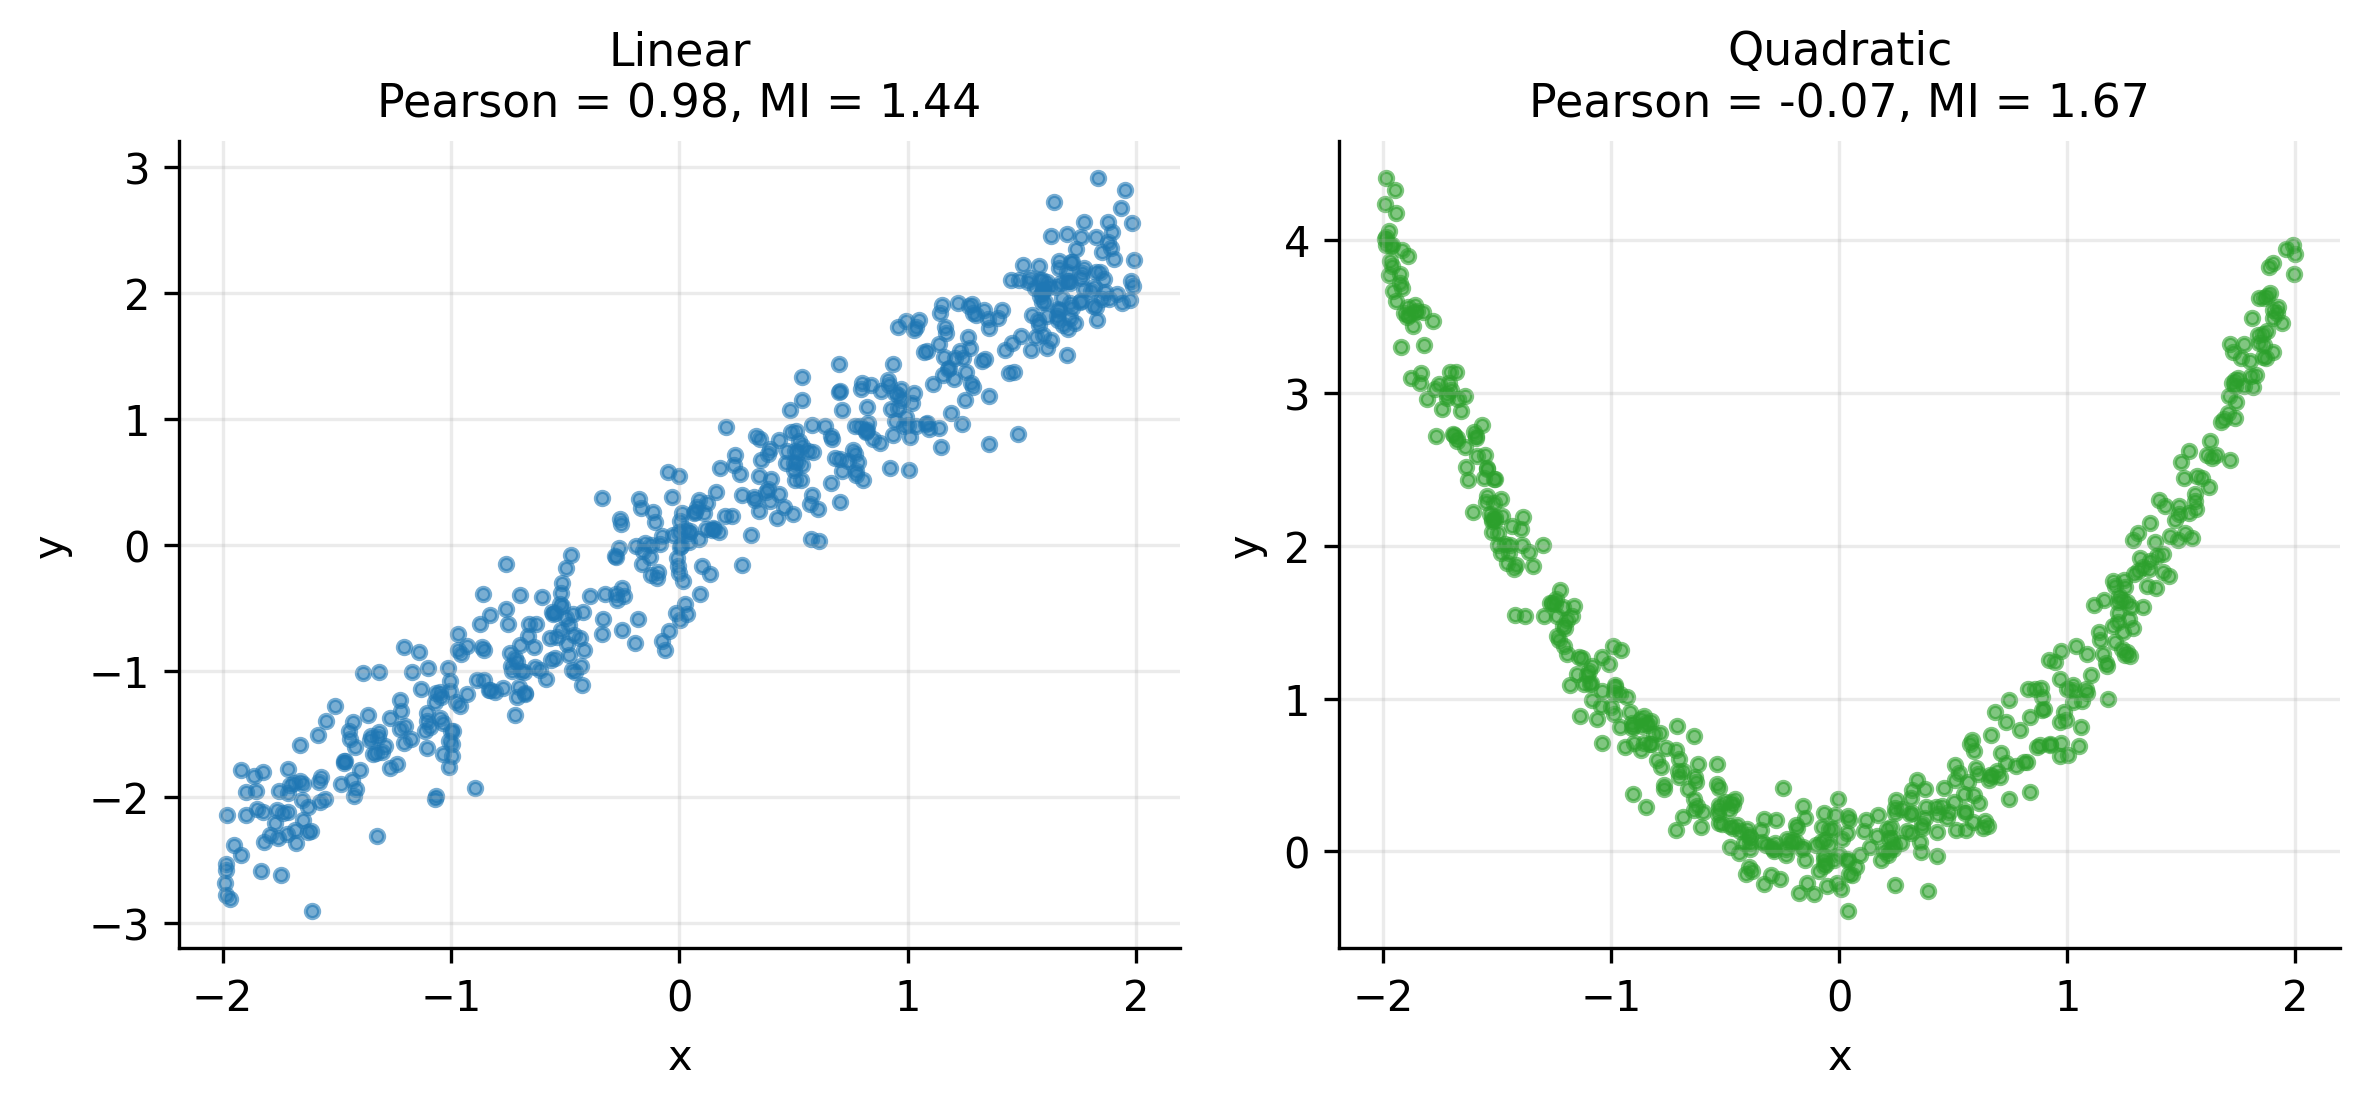
\includegraphics[width=0.95\linewidth]{figures/mi_vs_pearson.png}
\caption{Mutual information vs.\ Pearson on a linear relationship (both informative) and a quadratic relationship (Pearson collapses to $\approx 0$, MI remains high). MI characterises any form of statistical dependence, not just linear association.}
\label{fig:mi-vs-pearson}
\end{figure}

\subsubsection{8.1 Definitions}\label{81-definitions}

For discrete \(X, Y\) with joint PMF \(p_{XY}\): \[
I(X; Y) = \sum_{x, y} p_{XY}(x, y) \log \frac{p_{XY}(x, y)}{p_X(x) p_Y(y)}.
\]

For continuous \(X, Y\) with joint density: \[
I(X; Y) = \int \!\!\int p_{XY}(x, y) \log \frac{p_{XY}(x, y)}{p_X(x) p_Y(y)} \, dx \, dy.
\]

Equivalent formulations: \[
I(X; Y) = H(X) + H(Y) - H(X, Y) = H(Y) - H(Y \mid X) = H(X) - H(X \mid Y) = D_{\mathrm{KL}}(p_{XY} \,\|\, p_X p_Y).
\]

\subsubsection{8.2 Derivation of
equivalences}\label{82-derivation-of-equivalences}

\(H(X, Y) = -\sum p(x,y) \log p(x, y) = -\sum p(x,y)[\log p(y|x) + \log p(x)] = H(Y \mid X) + H(X)\).
Adding and subtracting \(H(Y)\):
\(H(X) + H(Y) - H(X, Y) = H(Y) - H(Y \mid X)\). The KL formulation falls
out by writing \(\log p(x, y) - \log p(x)p(y) = \log p(y|x)/p(y)\).

\subsubsection{8.3 Foundational
properties}\label{83-foundational-properties}

\begin{itemize}
\tightlist
\item
  \textbf{Non-negativity}: \(I(X; Y) \geq 0\), with equality iff
  \(X \perp Y\) (Gibbs inequality).
\item
  \textbf{Symmetry}: \(I(X; Y) = I(Y; X)\).
\item
  \textbf{Bounded by entropy}: \(I(X; Y) \leq \min(H(X), H(Y))\) for
  discrete variables.
\item
  \textbf{Invariance under invertible transformations}:
  \(I(g(X); h(Y)) = I(X; Y)\) for any bijective \(g, h\). A much larger
  invariance group than Pearson or Spearman.
\item
  \textbf{Chain rule}: \(I(X; Y, Z) = I(X; Y) + I(X; Z \mid Y)\).
\item
  \textbf{Data processing inequality}: if \(X \to Y \to Z\) is a Markov
  chain, \(I(X; Z) \leq I(X; Y)\).
\end{itemize}

\subsubsection{8.4 Estimation --- the hard
part}\label{84-estimation--the-hard-part}

\paragraph{Discrete plug-in}\label{discrete-plug-in}

For discrete \(X, Y\) with empirical joint \(\hat{p}_{xy} = n_{xy}/n\):
\[
\hat{I}_{\text{plug}} = \sum_{x, y} \hat{p}_{xy} \log \frac{\hat{p}_{xy}}{\hat{p}_x \hat{p}_y}.
\] \textbf{Bias}:
\(\mathbb{E}[\hat{I}_{\text{plug}}] - I \approx \frac{(K_{XY} - K_X - K_Y + 1)}{2n}\)
where \(K\)\textquotesingle s are the cardinalities of the supports
(Miller--Madow correction, 1955). For small \(n\) and large alphabets
the bias dominates; for \(n \gg K_{XY}\) it is negligible. Improved
estimators (Chao--Shen, Grassberger, NSB, James--Stein) reduce bias
further at the cost of complexity.

\paragraph{Continuous: binning}\label{continuous-binning}

Discretise each variable into \(b\) bins of equal width (or equal
probability), apply the discrete plug-in. Bias is highly sensitive to
bin width; rules of thumb include Sturges\textquotesingle{}
(\(b = \lceil \log_2 n + 1 \rceil\)), Freedman--Diaconis
(\(b = (\max - \min) / (2 \cdot \mathrm{IQR} \cdot n^{-1/3})\)), or
simply \(b \approx n^{1/3}\). Adaptive binning (e.g.,
MIC\textquotesingle s grid search, §9) improves on this.

\paragraph{\texorpdfstring{Continuous: \(k\)-NN
(Kraskov--Stögbauer--Grassberger, KSG
2004)}{Continuous: k-NN (Kraskov--Stögbauer--Grassberger, KSG 2004)}}\label{continuous-k-nn-kraskovstuxf6gbauergrassberger-ksg-2004}

The modern default. Algorithm:

\begin{enumerate}
\def\labelenumi{\arabic{enumi}.}
\tightlist
\item
  For each point \((x_i, y_i)\), find the \(k\)-th nearest neighbour in
  the joint space using Chebyshev (max-norm) distance:
  \(\varepsilon_i = \max(|x_i - x_{i,(k)}|, |y_i - y_{i,(k)}|)\).
\item
  Let \(n_x(i) = \#\{j \neq i : |x_j - x_i| < \varepsilon_i\}\) and
  \(n_y(i)\) analogously.
\item
  KSG-1 estimator: \[
  \hat{I}_{\text{KSG}} = \psi(k) - \frac{1}{n}\sum_{i=1}^{n}[\psi(n_x(i) + 1) + \psi(n_y(i) + 1)] + \psi(n),
  \] where \(\psi\) is the digamma function.
\end{enumerate}

Typical \(k \in \{3, 5, 7\}\) --- smaller \(k\) → lower bias, higher
variance. KSG handles continuous variables on their native scale (no
binning), is asymptotically unbiased, and is the implementation behind
\texttt{sklearn.feature\_selection.mutual\_info\_regression}.

\paragraph{Variational lower bounds (modern, for
high-dim)}\label{variational-lower-bounds-modern-for-high-dim}

For high-dimensional \(X, Y\) (text embeddings, image representations),
histogram and kNN methods break down. Variational estimators train a
neural network to maximise a lower bound on MI:

\begin{itemize}
\tightlist
\item
  \textbf{MINE} (Belghazi et al. 2018): Donsker--Varadhan bound,
  \(I(X; Y) \geq \mathbb{E}_{p_{XY}}[T] - \log \mathbb{E}_{p_X p_Y}[e^T]\).
\item
  \textbf{InfoNCE} (Oord et al. 2018):
  \(I(X; Y) \geq \log K - L_{\text{NCE}}\), where \(K\) is batch size
  --- bounded above by \(\log K\), which often dominates the bias.
\item
  \textbf{NWJ} (Nguyen--Wainwright--Jordan 2010):
  \(I(X; Y) \geq \mathbb{E}[T] - e^{-1}\mathbb{E}[e^T]\).
\end{itemize}

McAllester \& Stratos (2020) and Song \& Ermon (2020) show all
variational MI bounds have either large bias, large variance, or both
--- use them for representation learning, not for absolute MI estimates.

\subsubsection{8.5 The canonical "MI sees what Pearson misses"
example}\label{85-the-canonical-mi-sees-what-pearson-misses-example}

\begin{lstlisting}[language=Python]
import numpy as np
from sklearn.feature_selection import mutual_info_regression
from scipy.stats import pearsonr

rng = np.random.default_rng(0)
n = 2000
x = rng.uniform(-1, 1, size=n)
y = x ** 2 + 0.05 * rng.normal(size=n)  # quadratic

r, _ = pearsonr(x, y)
mi = mutual_info_regression(x.reshape(-1, 1), y, n_neighbors=3, random_state=0)[0]
print(f"Pearson r: {r:.4f}    MI (KSG): {mi:.4f}")
# Pearson ~ 0; MI ~ 1.5+ nats.
\end{lstlisting}

\subsubsection{8.6 Pitfalls}\label{86-pitfalls}

\begin{itemize}
\tightlist
\item
  \textbf{No sign}: MI cannot tell you positive vs negative association.
\item
  \textbf{Hard to compare across datasets} without a reference --- see
  NMI (§10).
\item
  \textbf{Curse of dimensionality}: KSG works well up to
  \textasciitilde5--8 dimensions per side; beyond that variance
  explodes.
\item
  \textbf{Sample-size hungry} for high MI: estimator variance scales
  with \(I\) itself; reliable estimation of \(I = 5\) nats requires
  substantially more data than \(I = 0.5\) nats.
\item
  \textbf{No closed-form null distribution}: significance is almost
  always assessed via permutation.
\end{itemize}

\subsubsection{8.7 When to use / when
not}\label{87-when-to-use--when-not}

\textbf{Use} when you want a \emph{fully general} measure of dependence,
have enough data (\(n \gtrsim 1000\) for continuous), and the
dimensionality is moderate. Feature selection where non-linearity is
expected; information-bottleneck analysis; communication theory;
representation learning (with caveats).

\textbf{Avoid} for small \(n\) with continuous variables and complex
marginal shapes --- estimator variance can swamp the signal. Use dCor or
HSIC instead.

\subsubsection{8.8 Cross-references}\label{88-cross-references}

For a normalised version see
\hyperref[10-normalized-mutual-information-nmi]{NMI}. For the
conditional version see
\hyperref[12-conditional-mutual-information-cmi]{CMI}. For a directional
time-series version see \hyperref[11-transfer-entropy]{Transfer
Entropy}. For modern alternatives with cleaner estimation theory see
\hyperref[13-distance-correlation-dcor]{dCor} and
\hyperref[16-hilbertschmidt-independence-criterion-hsic]{HSIC}.

\begin{center}\rule{0.5\linewidth}{0.5pt}\end{center}

\subsection{9. Maximal Information Coefficient
(MIC)}\label{9-maximal-information-coefficient-mic}

\subsubsection{9.1 Definition}\label{91-definition}

Reshef et al. (Science 2011). For continuous \(X, Y\) and grid sizes
\(a, b\) (number of bins on each axis), let \(I^*(X, Y; a, b)\) be the
maximum empirical mutual information over all \(a \times b\) partitions
of the data. Then \[
\mathrm{MIC}(X, Y) = \max_{ab \leq B(n)} \frac{I^*(X, Y; a, b)}{\log \min(a, b)},
\] with \(B(n) = n^{\alpha}\) (\(\alpha = 0.6\) by default).

\subsubsection{9.2 Intuition}\label{92-intuition}

For each "grid resolution," MIC searches for the \emph{most informative}
binning, normalises by the maximum-possible MI on a uniform
\(\min(a, b)\)-bin distribution, and reports the supremum over grid
sizes. The normalisation ensures \(\mathrm{MIC} \in [0, 1]\). The
grid-size cap \(B(n)\) prevents the search from overfitting at high
resolution.

\subsubsection{9.3 The "equitability" claim and the
controversy}\label{93-the-equitability-claim-and-the-controversy}

Reshef et al. claimed MIC has an \textbf{equitability} property: equally
noisy relationships of different functional types (linear, sinusoidal,
parabolic, exponential) should receive equal MIC scores. This made MIC
immediately appealing for exploratory screening of "any kind of
relationship."

Kinney \& Atwal (PNAS 2014) proved that \textbf{no nontrivial dependence
measure can be equitable in the original formalisation}: any measure
invariant under monotonic transforms and depending only on the
dependence structure (the copula) must violate equitability for some
pair of noise models. Subsequent work (Reshef et al. 2016) reformulated
equitability and introduced \textbf{MICe} (a much faster approximation),
but the controversy has dampened initial enthusiasm.

\subsubsection{9.4 Properties and
performance}\label{94-properties-and-performance}

\begin{itemize}
\tightlist
\item
  Range \([0, 1]\), symmetric, no sign.
\item
  \(\mathrm{MIC} = 1\) for noise-free functional relationships
  \emph{given sufficient \(n\)}.
\item
  \textbf{Lower statistical power than dCor and HSIC} on many smooth
  alternatives (Simon \& Tibshirani 2014 simulation benchmarks).
\item
  Computationally expensive: original MIC is \(O(n^{2.4})\); MICe is
  \(O(n^{1.2})\).
\end{itemize}

\subsubsection{9.5 Code}\label{95-code}

\begin{lstlisting}[language=Python]
# pip install minepy
from minepy import MINE
import numpy as np

rng = np.random.default_rng(0)
n = 1000
x = rng.uniform(0, 1, n)
y = np.sin(20 * x) + 0.2 * rng.normal(size=n)

mine = MINE(alpha=0.6, c=15)
mine.compute_score(x, y)
print(f"MIC = {mine.mic():.3f}")
\end{lstlisting}

\subsubsection{9.6 Pitfalls}\label{96-pitfalls}

\begin{itemize}
\tightlist
\item
  The "any kind of relationship" claim is \textbf{empirical}, not
  theoretical.
\item
  For most modern applications, \textbf{dCor or HSIC are simpler,
  faster, and more powerful}.
\item
  The grid-size cap \(\alpha = 0.6\) is a hyperparameter; results are
  sensitive to it for small \(n\).
\end{itemize}

\subsubsection{9.7 When to use}\label{97-when-to-use}

When you genuinely want a \([0, 1]\) scalar that returns 1 for any
noise-free functional relationship and you do not care about hypothesis
tests. Honest assessment: in 2026, prefer dCor or HSIC unless you have a
specific reason to want MIC\textquotesingle s equitability heuristic.

\begin{center}\rule{0.5\linewidth}{0.5pt}\end{center}

\subsection{10. Normalized Mutual Information
(NMI)}\label{10-normalized-mutual-information-nmi}

\subsubsection{10.1 Family of
definitions}\label{101-family-of-definitions}

NMI is not a single quantity --- it is at least four variants that
rescale MI into \([0, 1]\). With \(H\) denoting Shannon entropy:

{\def\LTcaptype{none} % do not increment counter
\begin{longtable}[]{@{}lll@{}}
\toprule\noalign{}
Variant & Formula & Notes \\
\midrule\noalign{}
\endhead
\bottomrule\noalign{}
\endlastfoot
Arithmetic mean & \(2 I(X;Y) / (H(X) + H(Y))\) & sklearn default \\
Geometric mean & \(I(X;Y) / \sqrt{H(X) H(Y)}\) & "Strehl-Ghosh" form \\
Min & \(I(X;Y) / \min(H(X), H(Y))\) & optimistic --- closest to 1 \\
Max & \(I(X;Y) / \max(H(X), H(Y))\) & pessimistic --- most
conservative \\
\end{longtable}
}

All four agree iff \(H(X) = H(Y)\).

\subsubsection{10.2 Why normalise}\label{102-why-normalise}

For raw MI, \(I(X; Y) = 2\) nats means different things on a 4-symbol
alphabet (where max is \(\log 4 \approx 1.39\)) versus a 100-symbol
alphabet (max \(\log 100 \approx 4.6\)). NMI factors this out, giving a
"fraction of shared entropy" interpretation.

\subsubsection{10.3 Cluster evaluation --- the dominant use
case}\label{103-cluster-evaluation--the-dominant-use-case}

NMI is the de facto standard for comparing two partitions \(U, V\) of
the same data. Treat cluster labels as random variables; compute NMI
between them; report.

Two important variants in this context:

\begin{itemize}
\tightlist
\item
  \textbf{Adjusted Mutual Information (AMI)}: subtracts the
  \emph{expected} NMI under random labellings, analogous to the Adjusted
  Rand Index. NMI rewards finer partitions (more clusters → higher
  entropy → easier to be informative); AMI corrects this. Vinh et al.
  (2010) is the canonical reference.
\item
  \textbf{Adjusted Rand Index (ARI)}: pair-counting analogue, sometimes
  preferred for partition comparison; AMI for information-theoretic, ARI
  for pair-counting.
\end{itemize}

\subsubsection{10.4 Code}\label{104-code}

\begin{lstlisting}[language=Python]
from sklearn.metrics import (
    normalized_mutual_info_score,
    adjusted_mutual_info_score,
    adjusted_rand_score,
)

labels_true = [0, 0, 1, 1, 2, 2, 3, 3]
labels_pred = [0, 0, 1, 1, 1, 1, 2, 2]
print(f"NMI (am):  {normalized_mutual_info_score(labels_true, labels_pred, average_method='arithmetic'):.3f}")
print(f"NMI (gm):  {normalized_mutual_info_score(labels_true, labels_pred, average_method='geometric'):.3f}")
print(f"AMI:       {adjusted_mutual_info_score(labels_true, labels_pred):.3f}")
print(f"ARI:       {adjusted_rand_score(labels_true, labels_pred):.3f}")
\end{lstlisting}

\subsubsection{10.5 Pitfalls}\label{105-pitfalls}

\begin{itemize}
\tightlist
\item
  \textbf{Different normalisations give different rankings} --- always
  report which one.
\item
  \textbf{NMI is biased upward toward finer partitions} when comparing
  clusterings of different cardinalities; \textbf{prefer AMI} for
  empirical clustering comparison.
\item
  \textbf{NMI for continuous variables} inherits all of
  MI\textquotesingle s estimation difficulties; it is overwhelmingly
  used in the discrete (clustering) setting.
\end{itemize}

\subsubsection{10.6 When to use}\label{106-when-to-use}

Clustering evaluation; comparing categorical-label distributions; any
setting where a normalised "fraction of shared information" is the
interpretable summary.

\begin{center}\rule{0.5\linewidth}{0.5pt}\end{center}

\subsection{11. Transfer Entropy}\label{11-transfer-entropy}

\subsubsection{11.1 Definition}\label{111-definition}

Schreiber (PRL 2000). For two time series \(X_t, Y_t\) and history
lengths \(k\) (for \(Y\)) and \(l\) (for \(X\)), \[
\mathrm{TE}_{X \to Y}(k, l) = \sum p(y_{t+1}, y_t^{(k)}, x_t^{(l)}) \log \frac{p(y_{t+1} \mid y_t^{(k)}, x_t^{(l)})}{p(y_{t+1} \mid y_t^{(k)})},
\] where \(y_t^{(k)} = (y_t, y_{t-1}, \dots, y_{t-k+1})\).

Equivalently,
\(\mathrm{TE}_{X \to Y} = I(Y_{t+1}; X_t^{(l)} \mid Y_t^{(k)})\): the
conditional mutual information between \(Y\)\textquotesingle s next
value and \(X\)\textquotesingle s past, given \(Y\)\textquotesingle s
own past.

\subsubsection{11.2 Intuition}\label{112-intuition}

By \emph{conditioning out the past of \(Y\)}, TE isolates the
\emph{additional} information about \(Y_{t+1}\) that comes from
\(X\)\textquotesingle s past --- over and above what
\(Y\)\textquotesingle s own dynamics already explain. This makes it
directional in a way ordinary MI is not.

\subsubsection{11.3 Relation to Granger
causality}\label{113-relation-to-granger-causality}

For jointly Gaussian, linear, stationary \((X_t, Y_t)\) processes,
transfer entropy is monotonically related to the Granger causality
\(F\)-statistic. Barnett, Barrett \& Seth (2009) showed: \[
\mathrm{TE}_{X \to Y} = \tfrac{1}{2} \log \frac{\mathrm{Var}(Y_{t+1} \mid Y_t^{(k)})}{\mathrm{Var}(Y_{t+1} \mid Y_t^{(k)}, X_t^{(l)})} = \tfrac{1}{2} \log F + \text{const},
\] i.e., TE is the \emph{nonlinear, non-parametric generalisation} of
Granger causality.

\subsubsection{11.4 Properties}\label{114-properties}

\begin{itemize}
\tightlist
\item
  \(\mathrm{TE}_{X \to Y} \geq 0\), with equality iff
  \(X\)\textquotesingle s past provides no additional information about
  \(Y_{t+1}\) beyond \(Y\)\textquotesingle s own past.
\item
  \textbf{Directional}:
  \(\mathrm{TE}_{X \to Y} \neq \mathrm{TE}_{Y \to X}\) in general; the
  difference is sometimes called the \emph{net} transfer entropy.
\item
  Can be normalised:
  \(\mathrm{nTE}_{X \to Y} = \mathrm{TE}_{X \to Y} / H(Y_{t+1} \mid Y_t^{(k)}) \in [0, 1]\).
\end{itemize}

\subsubsection{11.5 Estimation}\label{115-estimation}

\begin{itemize}
\tightlist
\item
  \textbf{Discrete or symbolised series}: bin or symbolise (rank short
  windows), apply discrete CMI estimator. Symbolic TE (Staniek \&
  Lehnertz 2008) is robust to choice of bin width.
\item
  \textbf{Continuous}: KSG-style estimator extended to conditional MI
  (Frenzel \& Pompe 2007).
\item
  \textbf{Effective TE}: subtract the bias estimated from shuffled
  surrogates. The reporting standard.
\end{itemize}

\subsubsection{11.6 Code}\label{116-code}

\begin{lstlisting}[language=Python]
# pip install PyInform
from pyinform.transferentropy import transfer_entropy
import numpy as np

rng = np.random.default_rng(0)
n = 5000
x = rng.integers(0, 2, size=n)
y = np.zeros(n, dtype=int)
for t in range(1, n):
    y[t] = x[t - 1] ^ rng.integers(0, 2)  # noisy XOR of x's past
te_x_to_y = transfer_entropy(x, y, k=1)
te_y_to_x = transfer_entropy(y, x, k=1)
print(f"TE X->Y: {te_x_to_y:.4f}    TE Y->X: {te_y_to_x:.4f}")
# X->Y should be much larger
\end{lstlisting}

\subsubsection{11.7 Pitfalls}\label{117-pitfalls}

\begin{itemize}
\tightlist
\item
  \textbf{Choice of history lengths} \((k, l)\) is consequential.
  Common: select by minimising AIC of the conditional density estimate,
  or use the Ragwitz criterion. Cross-validate where possible.
\item
  \textbf{Stationarity} is assumed; non-stationary series should be
  detrended or pre-processed (e.g. differencing).
\item
  \textbf{TE is not causality} in the interventional sense ---
  confounders can produce spurious TE. The terminology "directional
  information flow" is more accurate.
\item
  \textbf{Sample size}: reliable continuous-TE estimation typically
  requires \(n \gtrsim 10^4\).
\end{itemize}

\subsubsection{11.8 When to use}\label{118-when-to-use}

Neuroscience (information flow between brain regions in EEG/fMRI);
finance (lead-lag between assets); climate (teleconnections); any
time-series setting where direction matters and you cannot assume
linearity.

\begin{center}\rule{0.5\linewidth}{0.5pt}\end{center}

\subsection{12. Conditional Mutual Information
(CMI)}\label{12-conditional-mutual-information-cmi}

\subsubsection{12.1 Definition}\label{121-definition}

\[
I(X; Y \mid Z) = \mathbb{E}_Z[I(X; Y \mid Z = z)] = \iiint p(x, y, z) \log \frac{p(x, y \mid z)}{p(x \mid z)\, p(y \mid z)} \, dx\, dy\, dz.
\]

Equivalent:
\(I(X; Y \mid Z) = H(X \mid Z) + H(Y \mid Z) - H(X, Y \mid Z)\).

\subsubsection{12.2 Intuition}\label{122-intuition}

CMI measures the dependence between \(X\) and \(Y\) that \emph{remains}
after controlling for \(Z\). It is the information-theoretic analogue of
\textbf{partial correlation}: where partial correlation removes a linear
effect of \(Z\), CMI removes the \emph{full} statistical effect of
\(Z\), regardless of functional form.

\subsubsection{12.3 Key identities}\label{123-key-identities}

\begin{itemize}
\tightlist
\item
  \textbf{Independence characterisation}:
  \(I(X; Y \mid Z) = 0 \iff X \perp Y \mid Z\).
\item
  \textbf{Chain rule}: \(I(X; Y, Z) = I(X; Z) + I(X; Y \mid Z)\).
\item
  \textbf{Non-monotonicity in \(Z\)}: \(I(X; Y \mid Z)\) can be
  \emph{larger} or \emph{smaller} than \(I(X; Y)\) --- conditioning
  sometimes increases dependence (the "explaining away" effect, or
  Berkson\textquotesingle s paradox). Example: \(X, Y\) independent
  Bernoulli(1/2), \(Z = X \oplus Y\); then \(I(X; Y) = 0\) but
  \(I(X; Y \mid Z) > 0\).
\end{itemize}

\subsubsection{12.4 Estimation}\label{124-estimation}

\begin{itemize}
\tightlist
\item
  \textbf{kNN (Frenzel--Pompe 2007)}: extends KSG to the conditional
  case. Use Chebyshev neighbours in \((X, Y, Z)\) space; estimate from
  digamma functions of marginal counts.
\item
  \textbf{Copula-based}: estimate the conditional copula and integrate.
\item
  \textbf{Variational}: extends MINE/InfoNCE to conditional. High
  variance in practice.
\item
  \textbf{KCIT (Zhang et al. 2011)}: kernel-based CI test that produces
  a CMI-like statistic.
\end{itemize}

Estimator variance grows quickly with \(\dim(Z)\). For \(\dim(Z) > 3\),
expect difficulty.

\subsubsection{12.5 Causal discovery --- why it
matters}\label{125-causal-discovery--why-it-matters}

CI tests based on CMI (or its kernel proxies) are the workhorse of
\textbf{constraint-based causal discovery} (PC, FCI algorithms): learn
the skeleton of the underlying DAG by removing edges \((X, Y)\) for
which \(\exists S\) with \(X \perp Y \mid S\). Faithfulness assumption:
the only CIs in the data reflect those entailed by the DAG.

\subsubsection{12.6 Code}\label{126-code}

\begin{lstlisting}[language=Python]
# pip install npeet — Non-Parametric Entropy Estimation Toolkit (Ver Steeg)
import numpy as np
from npeet import entropy_estimators as ee

rng = np.random.default_rng(0)
n = 5000
z = rng.normal(size=(n, 1))
x = z + 0.5 * rng.normal(size=(n, 1))
y = z + 0.5 * rng.normal(size=(n, 1))
# X and Y are dependent through Z; should be independent given Z

mi_xy = ee.mi(x, y, k=5)
cmi_xy_given_z = ee.cmi(x, y, z, k=5)
print(f"I(X; Y)       = {mi_xy:.4f} (expect > 0)")
print(f"I(X; Y | Z)   = {cmi_xy_given_z:.4f} (expect ~ 0)")
\end{lstlisting}

\subsubsection{12.7 Pitfalls}\label{127-pitfalls}

\begin{itemize}
\tightlist
\item
  \textbf{Conditioning is expensive}: estimator variance is brutal when
  \(Z\) is high-dimensional.
\item
  \textbf{Faithfulness violations}: causal-discovery algorithms based on
  CMI assume that all and only the CI relations in the data reflect the
  causal graph. Generic faithfulness holds almost everywhere in
  parameter space but can fail at parameter "knife-edges" (e.g.,
  cancellation in linear systems).
\item
  \textbf{Significance testing}: no closed-form null; permutation must
  respect the conditioning, e.g. local permutation (Runge 2018).
\end{itemize}

\subsubsection{12.8 When to use}\label{128-when-to-use}

Causal discovery; partial-correlation-like analysis with non-linear
relationships; Markov-blanket feature selection (\(X_i\) is irrelevant
given the rest iff \(I(Y; X_i \mid X_{-i}) = 0\)); confounder
adjustment.

\begin{center}\rule{0.5\linewidth}{0.5pt}\end{center}

\section{Part III --- Geometric, Kernel, and Modern Independence
Measures}\label{part-iii--geometric-kernel-and-modern-independence-measures}

This part collects measures that share three philosophical commitments:
(1) they detect \emph{any} form of dependence, not just linear or
monotonic; (2) they admit clean theoretical characterisations of
independence; (3) they exploit rich representations of the data
(distance matrices, RKHS embeddings, rank structures) rather than
histograms of values. They are the modern statistician\textquotesingle s
answer to the limitations of Pearson and the estimation difficulties of
MI.

\subsection{13. Distance Correlation
(dCor)}\label{13-distance-correlation-dcor}

\begin{figure}[h]
\centering
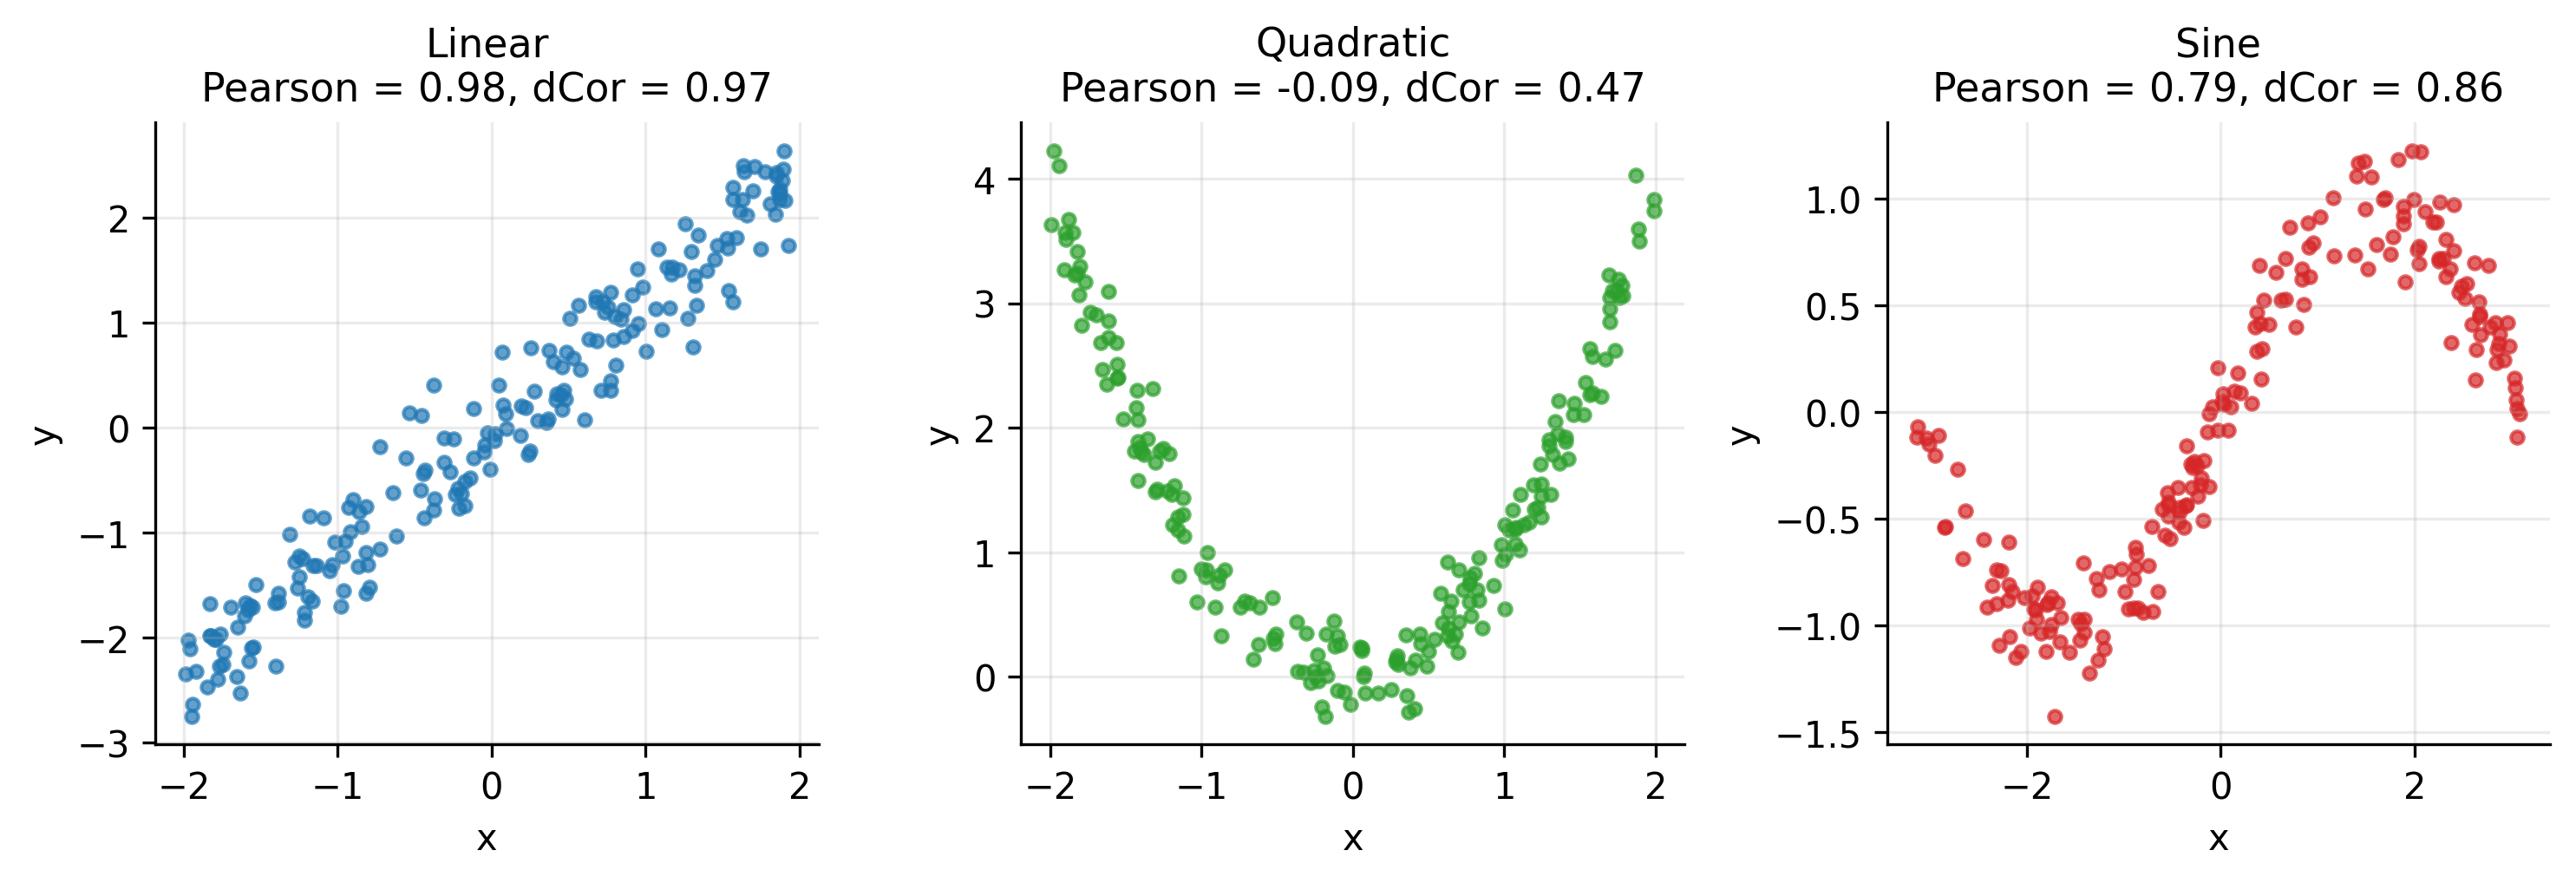
\includegraphics[width=0.95\linewidth]{figures/distance_correlation.png}
\caption{Distance correlation (dCor) vs.\ Pearson on three relationships. dCor remains positive in the quadratic and sine settings where Pearson drops to $\approx 0$. dCor is zero \emph{iff} the variables are independent, making it a true test of dependence.}
\label{fig:distance-correlation}
\end{figure}

\subsubsection{13.1 Definition (sample)}\label{131-definition-sample}

Székely, Rizzo, Bakirov (Annals of Statistics 2007). Given samples
\((x_i, y_i)\) for \(i = 1, \dots, n\) where \(x_i \in \mathbb{R}^p\),
\(y_i \in \mathbb{R}^q\):

\begin{enumerate}
\def\labelenumi{\arabic{enumi}.}
\tightlist
\item
  \textbf{Pairwise distance matrices}: \(a_{ij} = \|x_i - x_j\|\),
  \(b_{ij} = \|y_i - y_j\|\).
\item
  \textbf{Double-centring}:
  \(A_{ij} = a_{ij} - \bar{a}_{i\cdot} - \bar{a}_{\cdot j} + \bar{a}_{\cdot\cdot}\)
  where \(\bar{a}_{i\cdot} = \tfrac{1}{n}\sum_j a_{ij}\),
  \(\bar{a}_{\cdot j} = \tfrac{1}{n}\sum_i a_{ij}\),
  \(\bar{a}_{\cdot\cdot} = \tfrac{1}{n^2}\sum_{i,j} a_{ij}\). Similarly
  \(B_{ij}\).
\item
  \textbf{Distance covariance}:
  \(\mathrm{dCov}^2(X, Y) = \tfrac{1}{n^2}\sum_{i, j} A_{ij} B_{ij}\).
\item
  \textbf{Distance correlation}:
  \(\mathrm{dCor}(X, Y) = \mathrm{dCov}(X, Y) / \sqrt{\mathrm{dCov}(X, X)\, \mathrm{dCov}(Y, Y)}\).
\end{enumerate}

\subsubsection{13.2 Population definition (characteristic-function
form)}\label{132-population-definition-characteristic-function-form}

\[
\mathrm{dCov}^2(X, Y) = \int_{\mathbb{R}^{p+q}} |\varphi_{XY}(t, s) - \varphi_X(t) \varphi_Y(s)|^2 \, w(t, s) \, dt \, ds,
\] where \(w(t, s) = (c_p c_q \|t\|^{p+1} \|s\|^{q+1})^{-1}\) for
specific constants \(c_d = \pi^{(d+1)/2} / \Gamma((d+1)/2)\).

This is the L2 distance between the joint characteristic function and
the product of marginals --- a "spectral" measure of dependence.
\textbf{It equals zero iff \(X \perp Y\)} (which is exactly the
characterisation of independence by characteristic functions, P3). This
is the theoretical headline.

\subsubsection{13.3 Derivation of the equivalence between sample and
population
forms}\label{133-derivation-of-the-equivalence-between-sample-and-population-forms}

Astonishingly, the elaborate weighted-integral expression has the simple
distance-matrix computation as its sample analogue. The key identity
(Székely \& Rizzo 2007, Thm 7) is \[
\int \frac{1 - \cos(\langle t, x - y \rangle)}{c_p \|t\|^{p+1}} \, dt = \|x - y\|,
\] which lets you convert the integral over characteristic functions
into one over pairwise distances. The double-centring step removes the
marginal expectations and is what makes the empirical
\(\mathrm{dCov}^2\) a U-statistic-like quantity.

\subsubsection{13.4 Bias-corrected
estimator}\label{134-bias-corrected-estimator}

The V-statistic above has positive bias under independence. Székely \&
Rizzo (2014) introduced the \textbf{U-statistic dCov}: \[
U_n = \frac{1}{n(n-3)} \sum_{i \neq j} \tilde{A}_{ij} \tilde{B}_{ij},
\] where \(\tilde{A}_{ij}\) uses a modified centring (with \(n-2\),
\(n-1\), \(n\) in denominators instead of \(n\), \(n\), \(n\)). \(U_n\)
has expectation zero under independence and is the recommended statistic
for hypothesis testing.

\subsubsection{13.5 Properties}\label{135-properties}

\begin{itemize}
\tightlist
\item
  \(\mathrm{dCor} \in [0, 1]\) (vs \(\mathrm{dCov} \in [0, \infty)\)).
\item
  Symmetric, no sign.
\item
  Invariant under translations, orthogonal transformations, and global
  scaling of \(X\) and \(Y\) separately.
\item
  For univariate, jointly normal \((X, Y)\) with Pearson correlation
  \(\rho\):
  \(\mathrm{dCor}^2 = (\rho \arcsin\rho + \sqrt{1 - \rho^2} - \rho \arcsin(\rho/2) - \sqrt{4 - \rho^2} + 1)/(1 + \pi/3 - \sqrt{3})\).
  Numerically \(\mathrm{dCor} \approx |\rho|\) but slightly smaller.
  Equality at \(\rho = 0\) and \(\rho = \pm 1\).
\item
  Generalises to arbitrary metric spaces with negative-definite metrics
  (Lyons 2013).
\end{itemize}

\subsubsection{13.6 Asymptotic null
distribution}\label{136-asymptotic-null-distribution}

Under \(H_0: X \perp Y\), \[
n \cdot \mathrm{dCov}^2 \to_d \sum_{j=1}^{\infty} \lambda_j Z_j^2
\] where \(Z_j\) are iid standard normal and \(\lambda_j\) are
eigenvalues of a specific integral operator. This is a mixture of
\(\chi^2\); closed-form \(p\)-values are hard, so \textbf{permutation
tests} are the practical standard. A gamma approximation is often used.

\subsubsection{13.7 Fast algorithms}\label{137-fast-algorithms}

\begin{itemize}
\tightlist
\item
  \textbf{Generic case} (\(p, q > 1\)): \(O(n^2)\) time and memory.
  Limits practical use to \(n \lesssim 10^5\).
\item
  \textbf{Univariate case} (\(p = q = 1\)): Huo \& Székely (2016)
  achieved \(O(n \log n)\) via clever sorting + cumulative sums.
  Implemented in
  \texttt{dcor.distance\_covariance(x,\ y,\ method="mergesort")}.
\end{itemize}

\subsubsection{13.8 Code}\label{138-code}

\begin{lstlisting}[language=Python]
# pip install dcor
import numpy as np
import dcor

rng = np.random.default_rng(0)
n = 500
x = rng.uniform(-1, 1, size=n)
y_lin = 0.7 * x + 0.3 * rng.normal(size=n)
y_quad = x ** 2 + 0.05 * rng.normal(size=n)
y_indep = rng.normal(size=n)

for name, y in [("linear", y_lin), ("quadratic", y_quad), ("independent", y_indep)]:
    dc = dcor.distance_correlation(x, y)
    test = dcor.independence.distance_covariance_test(x, y, num_resamples=999, random_state=0)
    print(f"{name:12s}  dCor = {dc:.3f}  p = {test.pvalue:.3g}")
\end{lstlisting}

For the quadratic case, dCor will be substantially positive while
Pearson\textquotesingle s \(r\) is \textasciitilde0.

\subsubsection{13.9 Pitfalls}\label{139-pitfalls}

\begin{itemize}
\tightlist
\item
  \textbf{\(O(n^2)\) memory} makes dCor uncomfortable for
  \(n \gtrsim 10^5\) unless you use the fast univariate algorithm.
\item
  \textbf{Magnitude is hard to interpret in absolute terms} --- most
  useful as a ranking or as a test statistic. Do not transfer a Pearson
  rule-of-thumb ("0.3 weak, 0.7 strong") directly.
\item
  \textbf{Bias under independence} in the V-statistic form: use the
  bias-corrected estimator for tests.
\end{itemize}

\subsubsection{13.10 When to use}\label{1310-when-to-use}

Any general-purpose dependence detection in low-to-moderate sample sizes
where you want a single bounded scalar with a clean independence
characterisation. Particularly valuable for \textbf{multivariate} \(X\)
and \(Y\) --- compute dCor between a vector of features and a vector of
outcomes directly.

\begin{center}\rule{0.5\linewidth}{0.5pt}\end{center}

\subsection{14. Brownian Covariance}\label{14-brownian-covariance}

\subsubsection{14.1 Definition}\label{141-definition}

Let \(U(t), V(s)\) be independent standard Brownian motions on
\(\mathbb{R}^p, \mathbb{R}^q\), independent of \(X, Y\). The
\textbf{Brownian covariance} is \[
\mathrm{BCov}^2(X, Y) = \mathrm{Cov}^2\big(U(X), V(Y)\big),
\] where the outer covariance is taken jointly over \((X, Y, U, V)\).

\subsubsection{14.2 Equivalence to dCov}\label{142-equivalence-to-dcov}

\textbf{Theorem} (Székely \& Rizzo, Annals of Applied Statistics 2009):
\(\mathrm{BCov}^2(X, Y) = \mathrm{dCov}^2(X, Y)\).

\subsubsection{14.3 Why this equivalence
matters}\label{143-why-this-equivalence-matters}

Brownian covariance places dCov inside the \textbf{Gaussian process
covariance} framework: it is the covariance of two Brownian motions
evaluated at the data points. This is one of several routes to seeing
dCor as a special case of HSIC (§16) with a particular reproducing
kernel --- namely the \textbf{Brownian motion covariance kernel} \[
k(x, x') = \tfrac{1}{2}(\|x\| + \|x'\| - \|x - x'\|).
\]

The equivalence explains why dCor and HSIC frequently agree empirically
--- they are two parametrisations of the same broader family of
"energy-distance / kernel-mean-embedding" independence measures. In
particular, \textbf{distance covariance ≡ HSIC with the Brownian motion
kernel}.

\subsubsection{14.4 Practical
implication}\label{144-practical-implication}

You almost never compute Brownian covariance directly. You compute dCov,
which is equal to it, using the distance-matrix algorithm. The Brownian
covariance perspective is theoretical glue, valuable for understanding
\emph{why} dCor works and how it relates to kernel methods.

\subsubsection{14.5 Generalisations}\label{145-generalisations}

Sejdinovic et al. (2013) unified distance-based and kernel-based
independence statistics: for any \textbf{negative-definite metric}
\(d\), the corresponding "\(d\)-distance covariance" equals an HSIC with
kernel \(k(x, x') = d(x, x_0) + d(x_0, x') - d(x, x')\) for any choice
of origin \(x_0\). This shows that the difference between dCor and HSIC
is, fundamentally, just a choice of kernel.

\begin{center}\rule{0.5\linewidth}{0.5pt}\end{center}

\subsection{15. Kernel Canonical Correlation Analysis
(KCCA)}\label{15-kernel-canonical-correlation-analysis-kcca}

\subsubsection{15.1 From CCA to KCCA}\label{151-from-cca-to-kcca}

Classical \textbf{CCA} (Hotelling 1936): given two random vectors
\(X \in \mathbb{R}^p\), \(Y \in \mathbb{R}^q\), find linear combinations
\(\alpha^\top X\) and \(\beta^\top Y\) with maximum Pearson correlation:
\[
\rho_{\text{CCA}} = \sup_{\alpha, \beta} \frac{\alpha^\top \Sigma_{XY} \beta}{\sqrt{\alpha^\top \Sigma_{XX} \alpha \cdot \beta^\top \Sigma_{YY} \beta}}.
\] Solved by a generalised eigenvalue problem.

\textbf{KCCA} replaces linear combinations with arbitrary functions in
two RKHSs: \[
\rho_{\text{KCCA}} = \sup_{f \in \mathcal{H}_X, g \in \mathcal{H}_Y} \frac{\mathrm{Cov}(f(X), g(Y))}{\sqrt{\mathrm{Var}(f(X))\, \mathrm{Var}(g(Y))}}.
\]

\subsubsection{15.2 Sample computation}\label{152-sample-computation}

With kernel matrices \(K_X, K_Y\) (each \(n \times n\)) and centring
\(\tilde{K} = HKH\) where
\(H = I - \tfrac{1}{n}\mathbf{1}\mathbf{1}^\top\), KCCA reduces to the
generalised eigenvalue problem \[
\begin{pmatrix} 0 & \tilde{K}_X \tilde{K}_Y \\ \tilde{K}_Y \tilde{K}_X & 0 \end{pmatrix} \!\!\begin{pmatrix} \alpha \\ \beta \end{pmatrix} = \lambda \begin{pmatrix} (\tilde{K}_X + \varepsilon I)^2 & 0 \\ 0 & (\tilde{K}_Y + \varepsilon I)^2 \end{pmatrix} \!\!\begin{pmatrix} \alpha \\ \beta \end{pmatrix}.
\] The regularisation \(\varepsilon > 0\) is \textbf{critical} ---
without it, for any universal kernel the empirical KCCA always equals 1
(you can always find \(f, g\) such that \(f(X) = g(Y)\) exactly on the
data, since \(\phi_X(X)\) and \(\phi_Y(Y)\) span \(n\)-dimensional
subspaces in the RKHSs).

\subsubsection{15.3 Properties}\label{153-properties}

\begin{itemize}
\tightlist
\item
  Returns multiple canonical components (eigenvalues), useful for
  \textbf{multi-view representation learning}.
\item
  The leading canonical correlation provides a dependence measure but is
  \emph{not} an independence characterisation in the sharp HSIC sense
  without careful regularisation tuning.
\item
  Underlies \textbf{kernel ICA} (Bach \& Jordan 2002): minimising the
  leading canonical correlation under whitened sources separates
  independent components.
\end{itemize}

\subsubsection{15.4 Cost}\label{154-cost}

\(O(n^3)\) for the generalised eigenproblem on \(n \times n\) kernel
matrices, prohibitive beyond \(n \approx 10^4\) without \textbf{Nyström}
or \textbf{random Fourier feature} approximations.

\subsubsection{15.5 Code}\label{155-code}

\begin{lstlisting}[language=Python]
# pip install mvlearn
from mvlearn.embed import KCCA
import numpy as np

rng = np.random.default_rng(0)
n, d = 200, 10
shared = rng.normal(size=(n, 3))
X = shared @ rng.normal(size=(3, d)) + 0.5 * rng.normal(size=(n, d))
Y = np.tanh(shared @ rng.normal(size=(3, d))) + 0.5 * rng.normal(size=(n, d))

kcca = KCCA(n_components=2, regs=[1e-2, 1e-2], kernel="rbf")
embeddings = kcca.fit_transform([X, Y])
# Correlation between the two leading components
import numpy as np
print(f"KCCA component 1 corr: {np.corrcoef(embeddings[0][:, 0], embeddings[1][:, 0])[0, 1]:.3f}")
\end{lstlisting}

\subsubsection{15.6 Deep CCA}\label{156-deep-cca}

Andrew et al. (2013) replaced the kernel feature map with a neural
network, learning \(f, g\) jointly by gradient descent to maximise
canonical correlation in the network outputs. DCCA is now the standard
tool for non-linear multi-view representation learning at scale.

\subsubsection{15.7 When to use}\label{157-when-to-use}

Multi-view representation learning (audio + video, image + text),
finding shared non-linear structure between two feature sets, multimodal
fusion. For dependence \emph{testing}, prefer HSIC.

\begin{center}\rule{0.5\linewidth}{0.5pt}\end{center}

\subsection{16. Hilbert--Schmidt Independence Criterion
(HSIC)}\label{16-hilbertschmidt-independence-criterion-hsic}

\subsubsection{16.1 Definition
(population)}\label{161-definition-population}

Gretton, Bousquet, Smola, Schölkopf (ALT 2005). For characteristic
kernels \(k_X, k_Y\) with feature maps \(\phi_X, \phi_Y\) into RKHSs
\(\mathcal{H}_X, \mathcal{H}_Y\): \[
\mathrm{HSIC}(X, Y) = \|\mathbb{E}_{XY}[\phi_X(X) \otimes \phi_Y(Y)] - \mathbb{E}_X[\phi_X(X)] \otimes \mathbb{E}_Y[\phi_Y(Y)]\|_{\mathrm{HS}}^2.
\] This is the squared Hilbert--Schmidt norm of the
\textbf{cross-covariance operator} between the two RKHSs.

\subsubsection{16.2 Sample estimator}\label{162-sample-estimator}

With kernel matrices \(K, L\) (each \(n \times n\)) and centring matrix
\(H = I - \tfrac{1}{n}\mathbf{1}\mathbf{1}^\top\): \[
\widehat{\mathrm{HSIC}} = \frac{1}{(n - 1)^2}\, \mathrm{tr}(K H L H) = \frac{1}{(n - 1)^2}\, \mathrm{tr}(\tilde{K} \tilde{L}),
\] where \(\tilde{K} = HKH\) is the centred kernel matrix. The bias is
\(O(1/n)\); the unbiased \(V\)-statistic version (Song et al. 2012) is
preferred for hypothesis testing.

\subsubsection{16.3 Why it characterises
independence}\label{163-why-it-characterises-independence}

The mean embedding \(\mu_P = \mathbb{E}[\phi(X)]\) is, for
characteristic kernels, an \emph{injective} map from probability
distributions into the RKHS. HSIC measures the RKHS distance between the
embedding of the joint distribution and the embedding of the product of
marginals. With characteristic kernels (the Gaussian RBF is
characteristic on \(\mathbb{R}^d\)), this distance is zero iff the
distributions agree, i.e., iff \(X \perp Y\).

\subsubsection{16.4 Relationship to
dCor}\label{164-relationship-to-dcor}

With the Brownian-motion covariance kernel, HSIC equals dCov (Sejdinovic
et al. 2013, see §14). With a Gaussian kernel and judicious bandwidth,
HSIC behaves very similarly to dCor in practice. Both are members of a
broader family of "energy-distance / kernel-mean-embedding" independence
measures.

\subsubsection{16.5 Asymptotic null
distribution}\label{165-asymptotic-null-distribution}

Under \(H_0\) of independence, \[
n \cdot \widehat{\mathrm{HSIC}} \to_d \sum_{j} \lambda_j (Z_j^2 - 1),
\] a centred infinite sum of weighted \(\chi^2_1\). \textbf{Gamma
approximation}:
\(n \cdot \widehat{\mathrm{HSIC}} \sim \mathrm{Gamma}(\alpha, \beta)\)
with shape and rate matched to the moments of the null. Fast and
reasonably accurate for \(n \gtrsim 200\). \textbf{Permutation tests}
are the most common practical approach.

\subsubsection{16.6 Variants}\label{166-variants}

\begin{itemize}
\tightlist
\item
  \textbf{HSIC Lasso} (Yamada et al. 2014): non-linear feature selection
  by sparse regression on per-feature HSIC scores. The optimisation
  \(\min_\beta \|\bar{L} - \sum_i \beta_i \bar{K}_i\|_F^2 + \lambda \|\beta\|_1\)
  selects features with high HSIC to the target while avoiding
  redundancy.
\item
  \textbf{Centered Kernel Alignment (CKA)} (Cortes et al. 2012,
  popularised by Kornblith et al. 2019): the cosine version of HSIC, \[
  \mathrm{CKA}(X, Y) = \frac{\mathrm{HSIC}(X, Y)}{\sqrt{\mathrm{HSIC}(X, X) \cdot \mathrm{HSIC}(Y, Y)}}.
  \] CKA has become the dominant tool for comparing \textbf{neural
  network representations} across layers, training runs, and
  architectures.
\item
  \textbf{Conditional HSIC / HSCIC} (Park \& Muandet 2020): extends to
  conditional independence testing for causal discovery.
\item
  \textbf{Nyström / random-feature approximations} (Zhang et al. 2018)
  bring HSIC to large \(n\) at \(O(n m^2)\) cost for \(m \ll n\)
  landmarks.
\end{itemize}

\subsubsection{16.7 Code}\label{167-code}

\begin{lstlisting}[language=Python]
# pip install hyppo
import numpy as np
from hyppo.independence import Hsic, Dcorr

rng = np.random.default_rng(0)
n = 300
x = rng.uniform(-1, 1, size=(n, 1))
y = (x.ravel() ** 2 + 0.1 * rng.normal(size=n)).reshape(-1, 1)

hsic_stat, hsic_p = Hsic().test(x, y, reps=999, workers=-1)
dcor_stat, dcor_p = Dcorr().test(x, y, reps=999, workers=-1)
print(f"HSIC = {hsic_stat:.4f}  p = {hsic_p:.3g}")
print(f"dCor = {dcor_stat:.4f}  p = {dcor_p:.3g}")
\end{lstlisting}

\subsubsection{16.8 Kernel bandwidth
selection}\label{168-kernel-bandwidth-selection}

The \textbf{median heuristic} is the default: set \(\sigma\) to the
median Euclidean distance between sample pairs. Reasonable for most
uses; can be tuned by cross-validating the HSIC test power on permuted
data when stakes are high.

\subsubsection{16.9 Pitfalls}\label{169-pitfalls}

\begin{itemize}
\tightlist
\item
  \textbf{Kernel bandwidth choice} is consequential; results can vary
  materially across reasonable bandwidths.
\item
  \textbf{Power depends on whether the kernel is characteristic} on the
  marginal supports. For bounded data, RBF and Laplace are safe;
  polynomial kernels are not characteristic in general.
\item
  \textbf{\(O(n^2)\) memory} in the standard estimator; use Nyström for
  \(n > 10^5\).
\item
  \textbf{CKA\textquotesingle s interpretability for neural
  representations} has been challenged (Davari et al. 2023) --- it can
  be biased toward dimensions with large eigenvalues.
\end{itemize}

\subsubsection{16.10 When to use}\label{1610-when-to-use}

General-purpose independence testing; non-linear feature selection (HSIC
Lasso); comparing learned representations (CKA); structured-output
learning; anywhere you would reach for dCor.

\begin{center}\rule{0.5\linewidth}{0.5pt}\end{center}

\subsection{\texorpdfstring{17. Chatterjee\textquotesingle s Rank
Correlation
\(\xi\)}{17. Chatterjee\textquotesingle s Rank Correlation \textbackslash xi}}\label{17-chatterjees-rank-correlation-xi}

\begin{figure}[h]
\centering
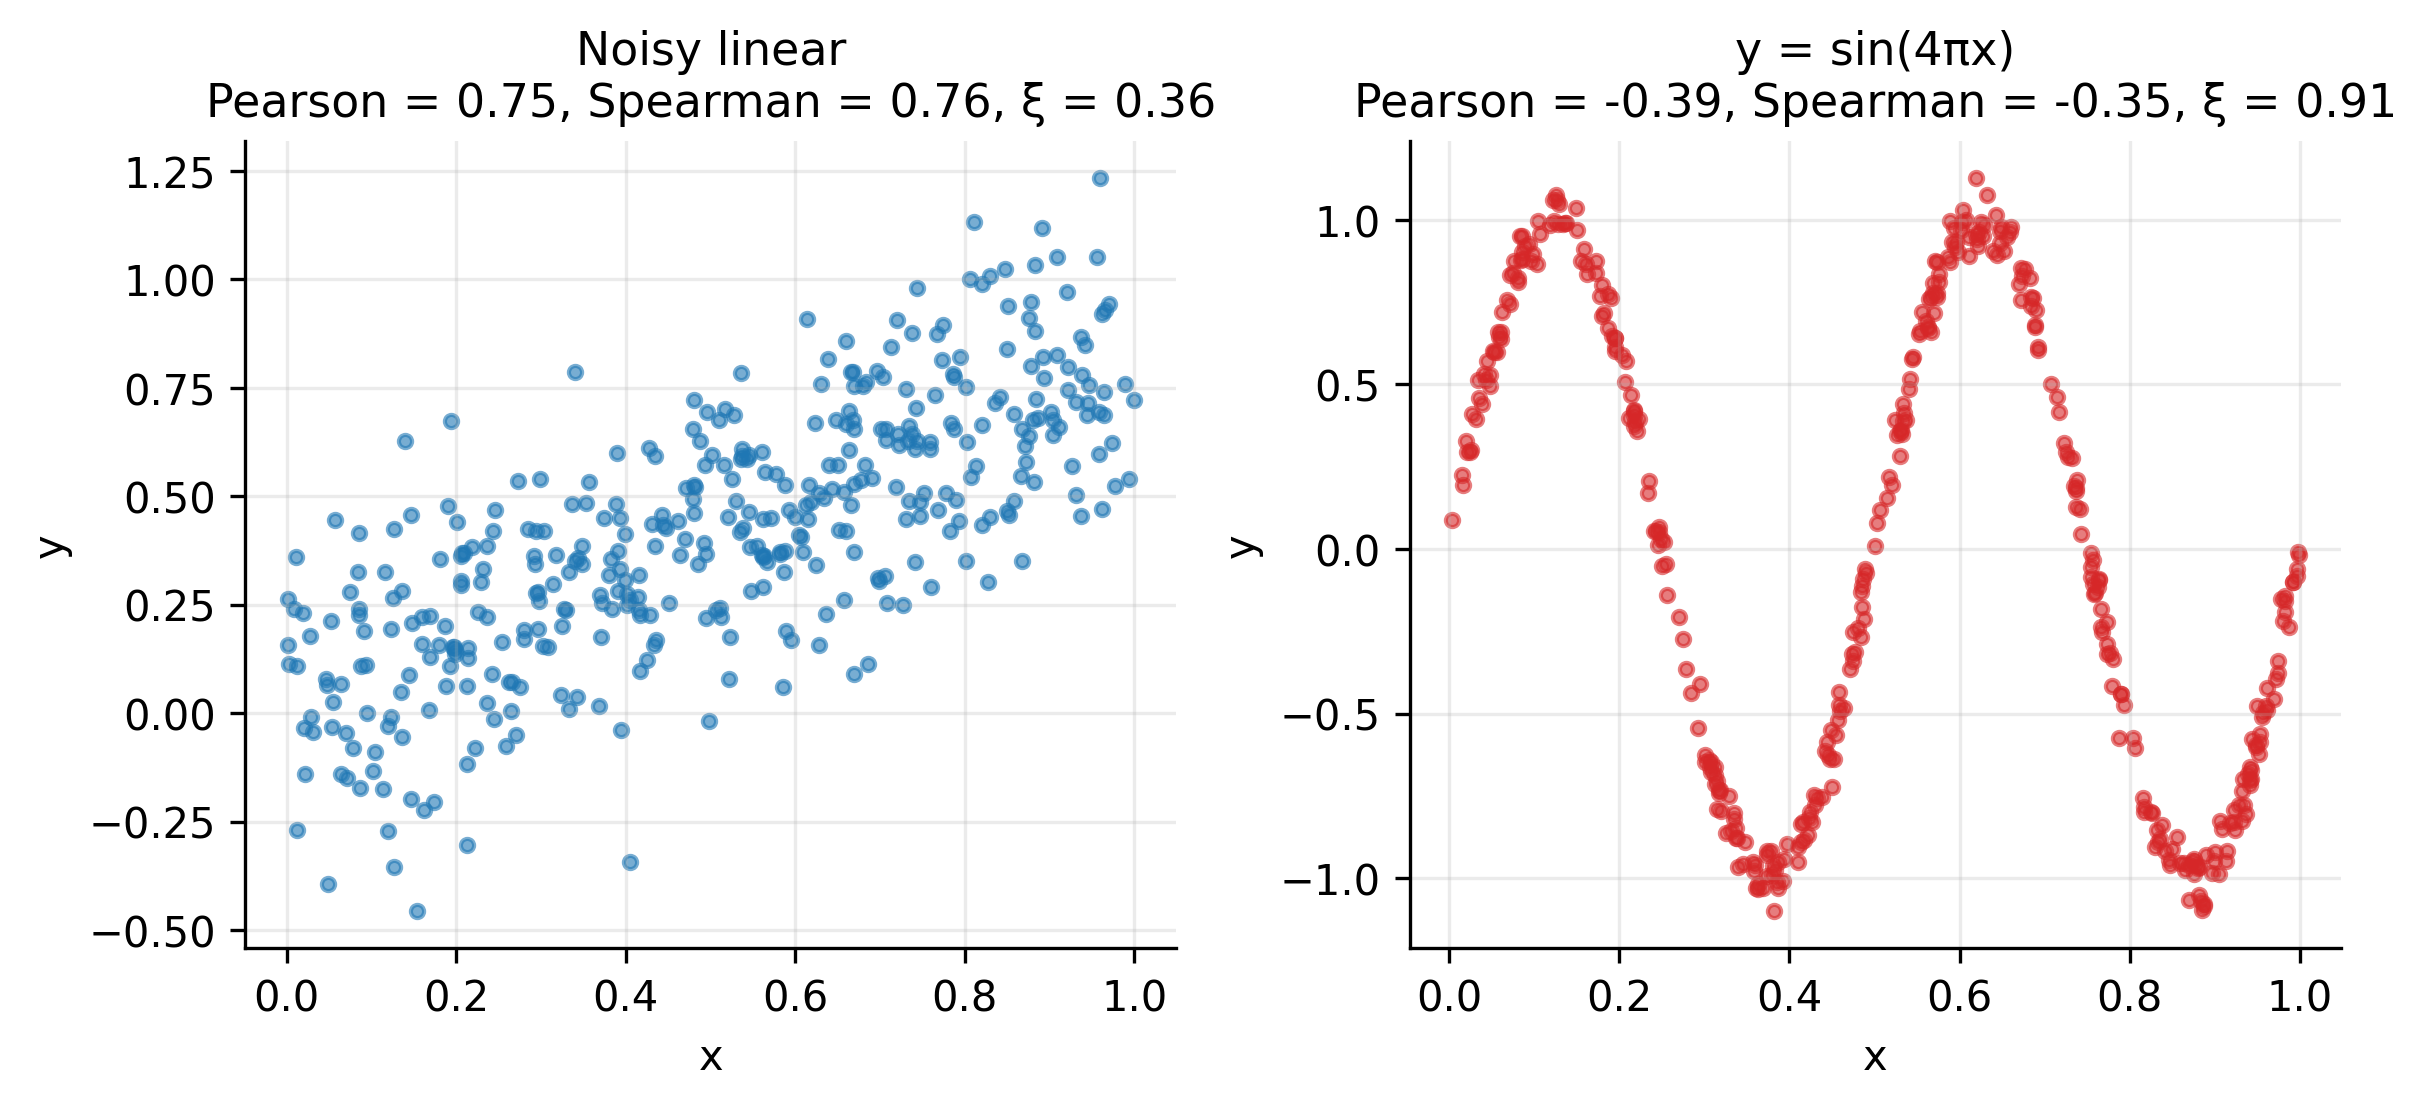
\includegraphics[width=0.95\linewidth]{figures/chatterjee_xi.png}
\caption{Chatterjee's $\xi$ on two cases. Left: a noisy linear trend; Pearson, Spearman, and $\xi$ all positive. Right: $y = \sin(4\pi x)$, where Pearson and Spearman both vanish but $\xi$ approaches its upper bound, signaling that $Y$ is a (deterministic) function of $X$.}
\label{fig:chatterjee-xi}
\end{figure}

\subsubsection{17.1 Definition}\label{171-definition}

Chatterjee (JASA 2020). Reorder the data so that
\(x_{(1)} \leq x_{(2)} \leq \dots \leq x_{(n)}\), with corresponding
\(y_{(1)}, \dots, y_{(n)}\). Let \(r_i\) denote the rank of \(y_{(i)}\)
in \(\{1, \dots, n\}\). Then (continuous, no ties): \[
\xi_n(X, Y) = 1 - \frac{3 \sum_{i=1}^{n-1} |r_{i+1} - r_i|}{n^2 - 1}.
\]

With ties on \(Y\), the corrected form is \[
\xi_n = 1 - \frac{n \sum_{i=1}^{n-1} |r_{i+1} - r_i|}{2 \sum_{i=1}^{n} \ell_i (n - \ell_i)},
\] where \(\ell_i\) is the number of \(j\) with
\(y_{(j)} \geq y_{(i)}\).

\subsubsection{17.2 Intuition}\label{172-intuition}

Sort observations by \(X\). If \(Y\) is a (possibly non-monotonic)
\textbf{function} of \(X\), then neighbouring \(Y\)-ranks
\(r_{i+1}, r_i\) are close to each other and the sum of jumps
\(\sum |r_{i+1} - r_i|\) is small. If \(Y\) is independent of \(X\),
neighbouring \(Y\)-ranks are roughly uniform on \(\{1, \dots, n\}\) and
the sum of jumps is large (of order \(n^2/3\)).

\subsubsection{17.3 Theoretical
headlines}\label{173-theoretical-headlines}

\begin{itemize}
\tightlist
\item
  \textbf{Population version} (continuous, no ties): \[
  \xi(X, Y) = \frac{\int \mathrm{Var}\{\mathbb{E}[\mathbb{1}\{Y \geq t\} \mid X]\}\, d\mu(t)}{\int \mathrm{Var}\{\mathbb{1}\{Y \geq t\}\}\, d\mu(t)} \in [0, 1].
  \]
\item
  \(\xi(X, Y) = 0\) iff \(X \perp Y\).
\item
  \(\xi(X, Y) = 1\) iff \(Y\) is a \emph{measurable function} of \(X\).
\item
  \(\xi\) is \textbf{asymmetric}: \(\xi(X, Y) \neq \xi(Y, X)\) in
  general. It measures the extent to which \(Y\) is a function of \(X\),
  not the other way around. \textbf{Different from any classical
  correlation.}
\item
  \textbf{Closed-form asymptotic null}: under independence with
  continuous distributions, \[
  \sqrt{n}\, \xi_n \to_d \mathcal{N}(0, 2/5).
  \] This enables closed-form \(p\)-values without permutations ---
  unique among the modern "any-shape" measures.
\end{itemize}

\subsubsection{17.4 Why "asymmetric" is a
feature}\label{174-why-asymmetric-is-a-feature}

Suppose \(Y = f(X)\) for some many-to-one function \(f\) (e.g.
\(Y = X^2\)). Knowing \(X\) determines \(Y\) --- so \(\xi(X, Y) \to 1\).
But knowing \(Y\) leaves \(X\) undetermined (each \(Y\) corresponds to
two \(X\)\textquotesingle s) --- so \(\xi(Y, X) < 1\). This asymmetry is
precisely what makes \(\xi\) a \emph{functional dependence detector},
suitable as a screening tool in causal discovery.

\subsubsection{17.5 Properties}\label{175-properties}

\begin{itemize}
\tightlist
\item
  Range: \([-1/2, 1]\) in finite samples (population: \([0, 1]\));
  negative values are noise.
\item
  Invariant under strictly increasing transformations of \(X\) or \(Y\)
  separately.
\item
  Lower power than dCor/HSIC for some smooth alternatives (linear) but
  uniquely capable of detecting \textbf{functional non-monotonic}
  relationships and providing a closed-form null.
\end{itemize}

\subsubsection{17.6 Variants and
extensions}\label{176-variants-and-extensions}

\begin{itemize}
\tightlist
\item
  \textbf{Conditional Chatterjee} (Azadkia \& Chatterjee, Annals of
  Statistics 2021): \(\xi(Y, Z \mid X)\), enabling variable selection in
  regression settings.
\item
  \textbf{Multi-variable} (Chatterjee 2022; Lin \& Han 2023):
  generalisation to \(\xi(\mathbf{X}, Y)\) with
  \(\mathbf{X} \in \mathbb{R}^p\).
\item
  \textbf{Lin--Han modification}: improved finite-sample properties
  relative to the original conservative estimator.
\end{itemize}

\subsubsection{17.7 Code}\label{177-code}

\begin{lstlisting}[language=Python]
# pip install xicor
from xicor.xicor import Xi
import numpy as np

rng = np.random.default_rng(0)
n = 1000
x = rng.uniform(0, 1, n)
y_func = np.sin(10 * x) + 0.05 * rng.normal(size=n)
y_indep = rng.normal(size=n)

print("Y = sin(10X) + noise:")
xi = Xi(x, y_func); print(f"  xi(X,Y) = {xi.correlation:.3f}  p = {xi.pval_asymptotic(ties=False):.3g}")
xi_rev = Xi(y_func, x); print(f"  xi(Y,X) = {xi_rev.correlation:.3f}  (asymmetric!)")

print("\nIndependent:")
xi = Xi(x, y_indep); print(f"  xi(X,Y) = {xi.correlation:.3f}  p = {xi.pval_asymptotic(ties=False):.3g}")
\end{lstlisting}

\subsubsection{17.8 Pitfalls}\label{178-pitfalls}

\begin{itemize}
\tightlist
\item
  \textbf{Asymmetric} --- be deliberate about which variable plays which
  role. Convention: \(\xi(X, Y)\) measures "\(Y\) is a function of
  \(X\)".
\item
  \textbf{Slower convergence} than parametric correlations; needs
  reasonably large \(n\) to detect weak dependence.
\item
  \textbf{Original estimator is conservative}; the Lin--Han modification
  has better finite-sample power.
\item
  \textbf{Asymptotic null assumes continuity} with no ties; for heavy
  ties use the tied-data correction or permutation.
\end{itemize}

\subsubsection{17.9 When to use}\label{179-when-to-use}

Functional-dependence detection (especially non-monotonic); screening
for unusual relationships when you cannot afford permutation tests;
replacement for Spearman / Kendall when you suspect non-monotonic
structure; causal-discovery-style screening for "is \(Y\) a function of
\(X\)?" hypotheses.

\begin{center}\rule{0.5\linewidth}{0.5pt}\end{center}

\section{Part IV --- Model-Agnostic Feature
Importance}\label{part-iv--model-agnostic-feature-importance}

The measures up to here summarise the \emph{joint distribution} of
variables. Starting now, the question changes: we no longer ask "is
\(X\) associated with \(Y\)?" but "\textbf{how much does this trained
model rely on \(X\) to make its predictions?}" --- a related but
importantly different question. A feature with high data-distribution
dependence on the target may be ignored by the model (perhaps because
the model uses a stronger proxy); a feature with no marginal association
may matter to the model through interactions; a feature that adds no
out-of-sample value may still acquire high in-sample importance under
any of these methods. Read this part with the model-vs-data distinction
always in mind.

\subsection{18. SHAP (SHapley Additive
exPlanations)}\label{18-shap-shapley-additive-explanations}

\begin{figure}[h]
\centering
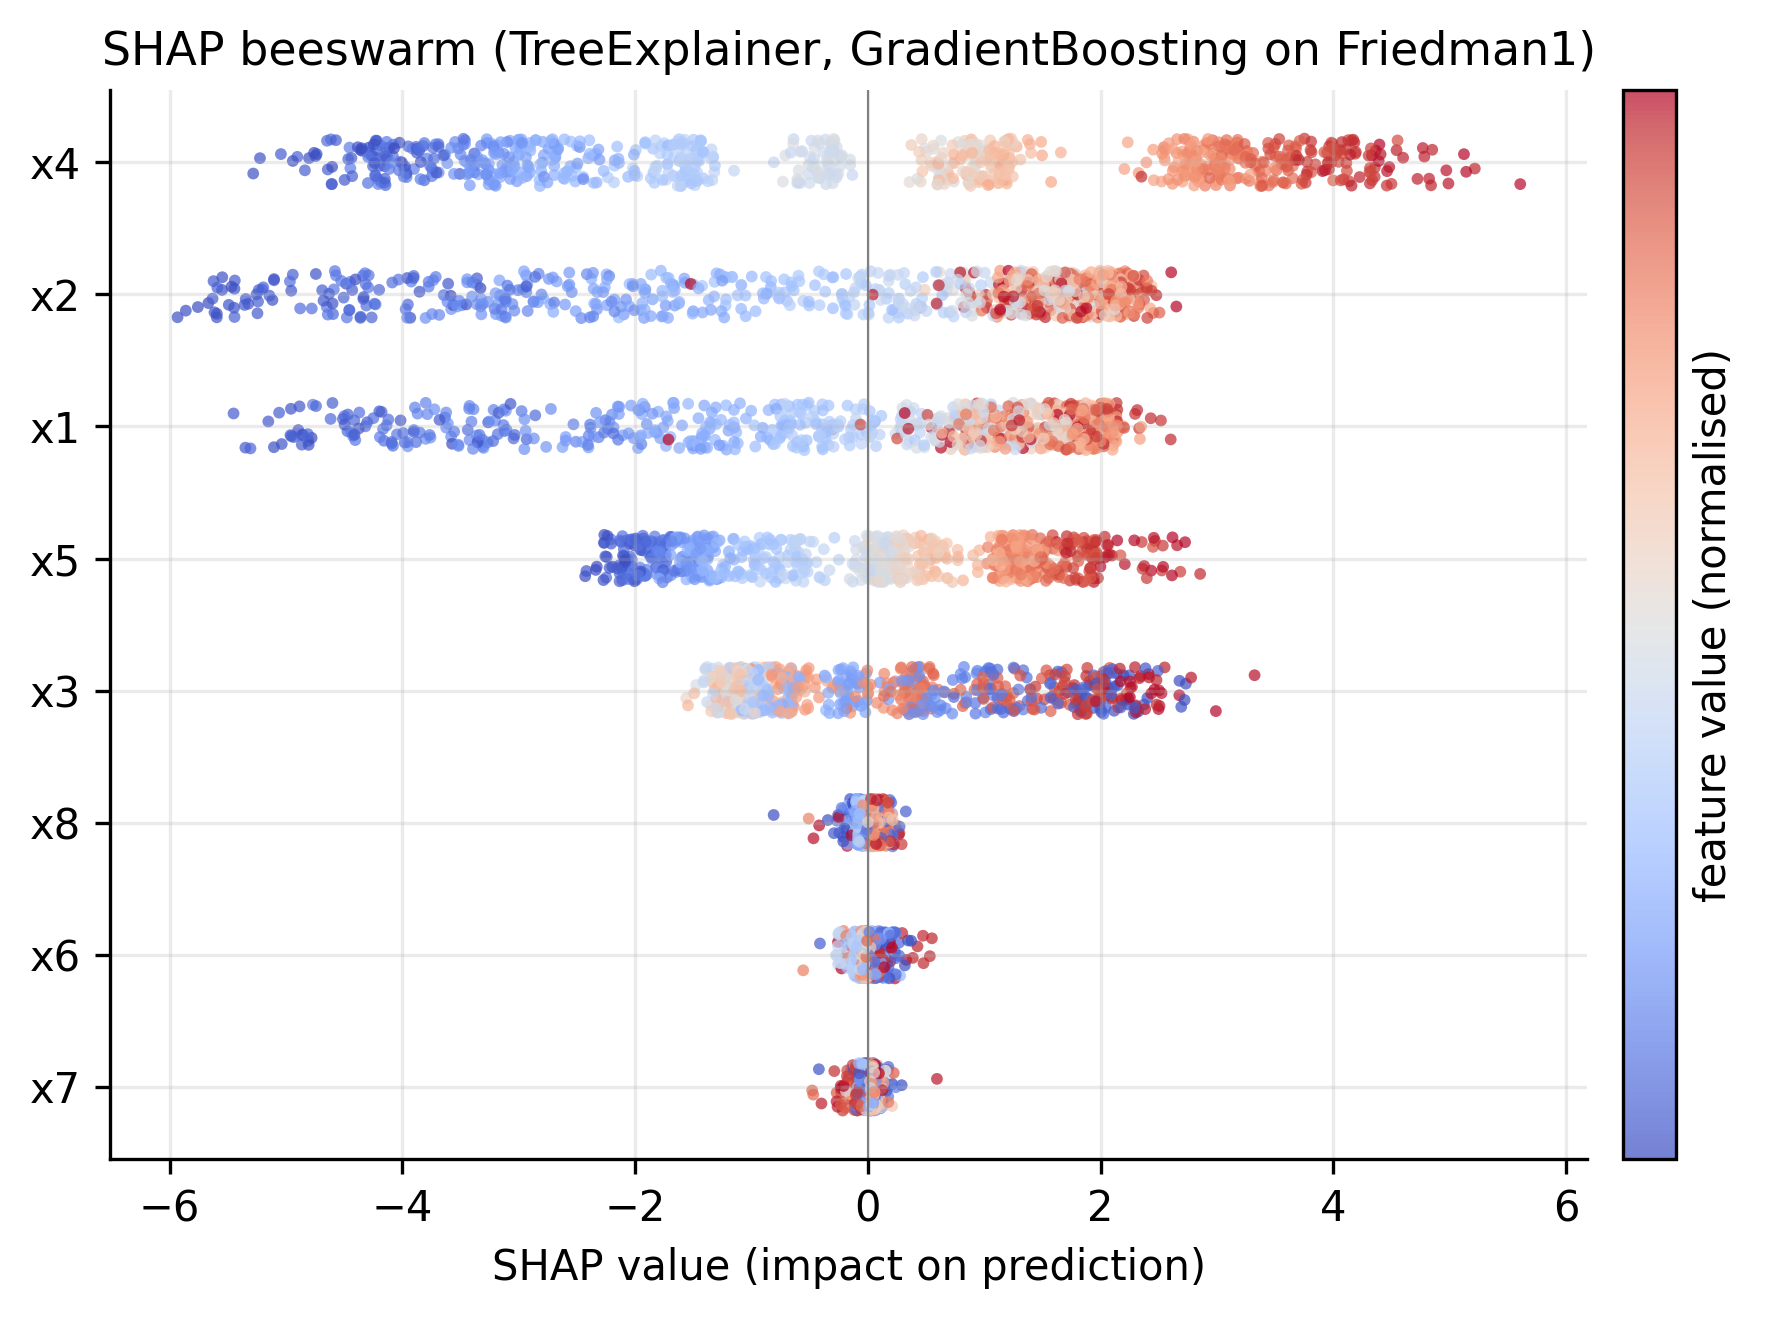
\includegraphics[width=0.85\linewidth]{figures/shap_summary.png}
\caption{SHAP beeswarm summary for a Gradient Boosting regressor on the Friedman~1 dataset. Each dot is one observation's SHAP value for a given feature; horizontal position is the impact on the prediction; color encodes the (normalised) feature value. Features are ordered by mean $|{\rm SHAP}|$.}
\label{fig:shap-summary}
\end{figure}

\subsubsection{18.1 Setup}\label{181-setup}

Lundberg \& Lee (NeurIPS 2017) unified a decade of additive
feature-attribution methods (LIME, DeepLIFT, Integrated Gradients,
Tree-SHAP, Shapley sampling) under the framework of \textbf{Shapley
values} from cooperative game theory (P9). Treat features as players in
a game where the "payout" is the model\textquotesingle s prediction; the
Shapley value of each feature is its fair share of the prediction
relative to a baseline.

\subsubsection{18.2 Formal definition}\label{182-formal-definition}

For a model \(f\), an input \(\mathbf{x} = (x_1, \dots, x_p)\), and a
value function \(v: 2^{\{1, \dots, p\}} \to \mathbb{R}\) with \(v(S)\)
representing the model\textquotesingle s prediction when only features
in \(S\) are "known": \[
\phi_i(\mathbf{x}) = \sum_{S \subseteq N \setminus \{i\}} \frac{|S|!\, (p - |S| - 1)!}{p!} \left[ v(S \cup \{i\}) - v(S) \right].
\]

The Shapley values satisfy four axioms (efficiency, symmetry, dummy,
additivity --- see P9) and decompose the prediction exactly: \[
f(\mathbf{x}) = \mathbb{E}[f(\mathbf{X})] + \sum_{i=1}^{p} \phi_i(\mathbf{x}).
\]

\subsubsection{18.3 The value function: interventional vs
observational}\label{183-the-value-function-interventional-vs-observational}

The choice of value function \(v(S)\) --- what it means for "features in
\(S\) are known" --- is the most subtle and consequential decision in
SHAP.

\begin{itemize}
\item
  \textbf{Interventional} (a.k.a. "marginal") SHAP: \[
  v(S) = \mathbb{E}_{X_{\bar{S}}}[f(\mathbf{x}_S, X_{\bar{S}})]
  \] where \(\bar{S} = N \setminus S\). Features outside \(S\) are drawn
  from their \textbf{marginal} distribution, breaking any correlation
  with features in \(S\).
\item
  \textbf{Observational} (a.k.a. "conditional") SHAP: \[
  v(S) = \mathbb{E}[f(\mathbf{X}) \mid X_S = \mathbf{x}_S]
  \] Features outside \(S\) are drawn from their \textbf{conditional}
  distribution given the observed values.
\end{itemize}

The two differ whenever features are correlated. Janzing, Minorics \&
Blöbaum (AISTATS 2020) argued the \textbf{interventional} formulation is
the right one for \emph{causal/explanatory} questions; the
\textbf{conditional} form reflects predictive associations under the
data distribution but can attribute importance to features the model
never actually uses (if a feature is correlated with one the model does
use, it inherits credit).

Practical implication: TreeSHAP\textquotesingle s two modes
(\texttt{feature\_perturbation="tree\_path\_dependent"} ≈ observational;
\texttt{feature\_perturbation="interventional"} ≈ interventional) can
give meaningfully different rankings. Pick deliberately.

\subsubsection{18.4 Estimators}\label{184-estimators}

\begin{itemize}
\tightlist
\item
  \textbf{KernelSHAP} (model-agnostic): weighted linear regression on
  sampled coalitions. The weights
  \(w(|S|) = \frac{p - 1}{\binom{p}{|S|} |S| (p - |S|)}\) are derived to
  recover Shapley values exactly. Slow (\(O(2^p)\) exact,
  \(O(K \cdot \text{infer})\) sampled).
\item
  \textbf{TreeSHAP} (Lundberg et al. 2018): polynomial-time
  \textbf{exact} SHAP for tree ensembles. Algorithm complexity
  \(O(TLD^2)\) where \(T\) is trees, \(L\) leaves per tree, \(D\) depth.
  The practical workhorse for XGBoost / LightGBM / sklearn forests.
\item
  \textbf{DeepSHAP / GradientSHAP}: approximations for neural networks;
  relate to DeepLIFT and Integrated Gradients respectively.
\item
  \textbf{LinearSHAP}: closed form for linear models; for a linear model
  \(f(\mathbf{x}) = \beta_0 + \sum_i \beta_i x_i\),
  \(\phi_i(\mathbf{x}) = \beta_i (x_i - \mathbb{E}[X_i])\) under the
  interventional value function.
\end{itemize}

\subsubsection{18.5 Global aggregation}\label{185-global-aggregation}

Per-prediction \(\phi_i(\mathbf{x})\) can be aggregated to global
importance:

\begin{itemize}
\tightlist
\item
  \textbf{Mean absolute SHAP}:
  \(\bar{\phi}_i = \tfrac{1}{n}\sum_j |\phi_i(\mathbf{x}_j)|\).
\item
  \textbf{Mean squared SHAP}:
  \(\tfrac{1}{n}\sum_j \phi_i(\mathbf{x}_j)^2\).
\item
  \textbf{SHAP summary plot (beeswarm)}: arguably the most informative
  single visualisation in modern ML interpretability --- one row per
  feature, one dot per training example, x-position = SHAP value, colour
  = feature value. Reveals direction of effect, heterogeneity,
  interactions.
\end{itemize}

\subsubsection{18.6 Code}\label{186-code}

\begin{lstlisting}[language=Python]
# pip install shap xgboost
import shap
import xgboost as xgb
import numpy as np

rng = np.random.default_rng(0)
n, p = 1000, 5
X = rng.normal(size=(n, p))
y = 2 * X[:, 0] + X[:, 1] ** 2 - X[:, 2] * X[:, 3] + 0.5 * rng.normal(size=n)

model = xgb.XGBRegressor(n_estimators=200, max_depth=4).fit(X, y)

explainer = shap.TreeExplainer(model, feature_perturbation="interventional", data=X)
shap_values = explainer.shap_values(X)

# Per-prediction
print("First prediction breakdown:")
print(f"  baseline      = {explainer.expected_value:.3f}")
print(f"  sum of SHAPs  = {shap_values[0].sum():.3f}")
print(f"  prediction    = {model.predict(X[:1])[0]:.3f}")

# Global
global_importance = np.abs(shap_values).mean(axis=0)
for i, imp in enumerate(global_importance):
    print(f"  feature {i}: {imp:.4f}")
\end{lstlisting}

\subsubsection{18.7 Pitfalls}\label{187-pitfalls}

\begin{itemize}
\tightlist
\item
  \textbf{Correlated features cause unstable attributions.} Shapley
  values split credit between correlated features in ways that are hard
  to predict; small data perturbations can move the split substantially.
  Group correlated features and report group-level Shapley values (Aas
  et al. 2021) for stability.
\item
  \textbf{Interventional SHAP can query the model at unrealistic points}
  (e.g. \(\text{age} = 5, \text{salary} = \$200{,}000\)); the model may
  behave erratically there, and that behaviour shows up in the SHAP
  values.
\item
  \textbf{SHAP explains the model, not the world.} A feature with high
  SHAP is one the model uses; it is not necessarily causally relevant.
\item
  \textbf{Computational cost}: KernelSHAP is \(O(2^p)\) exact,
  prohibitive beyond \textasciitilde10 features; TreeSHAP is polynomial
  but non-trivial for deep deep ensembles (hundreds of trees, depth
  10+).
\item
  \textbf{Sampling variance} --- KernelSHAP attributions are noisy
  estimates; reproducibility requires fixed seeds and enough samples
  (typically \(\geq 1000\)).
\end{itemize}

\subsubsection{18.8 When to use}\label{188-when-to-use}

Per-prediction explanations in regulated industries (credit, healthcare,
insurance); global feature ranking when you have a tree ensemble
(TreeSHAP is fast and exact); communicating model behaviour to
stakeholders via summary plots; identifying buggy features (a feature
that "should" be irrelevant showing up with high SHAP magnitude is a
strong leakage signal).

\begin{center}\rule{0.5\linewidth}{0.5pt}\end{center}

\subsection{19. Permutation Feature Importance
(PFI)}\label{19-permutation-feature-importance-pfi}

\subsubsection{19.1 Algorithm}\label{191-algorithm}

\begin{enumerate}
\def\labelenumi{\arabic{enumi}.}
\tightlist
\item
  Compute the baseline model performance
  \(s_0 = \mathrm{score}(f, \mathcal{D})\) on a held-out dataset
  \(\mathcal{D}\).
\item
  For each feature \(i \in \{1, \dots, p\}\):

  \begin{itemize}
  \tightlist
  \item
    Shuffle the column \(X_i\) across rows of \(\mathcal{D}\), breaking
    its relationship with \(Y\) and with the other features.
  \item
    Re-score the model on the permuted data: \(s_i\).
  \end{itemize}
\item
  PFI of feature \(i\) = \(s_0 - s_i\) (loss-style; reverse sign if
  higher score = worse).
\item
  Repeat across multiple permutations; report mean and standard
  deviation.
\end{enumerate}

\subsubsection{19.2 Intuition}\label{192-intuition}

"How much worse does the model become if I destroy this
feature\textquotesingle s signal but keep its marginal distribution
intact?"

\subsubsection{19.3 Properties}\label{193-properties}

\begin{itemize}
\tightlist
\item
  \textbf{Model-agnostic} --- works for any predictor.
\item
  Reflects \textbf{the model\textquotesingle s use of the feature}, not
  the joint distribution of \(X_i, Y\).
\item
  Computed on \textbf{test/validation data} = generalisation-relevant
  importance.
\item
  Computed on \textbf{training data} ≈ memorisation; a feature can show
  high training PFI even if it adds no out-of-sample value. Always use
  held-out data unless you have a specific reason not to.
\end{itemize}

\subsubsection{19.4 The correlated-features
trap}\label{194-the-correlated-features-trap}

Suppose \(X_1, X_2\) are perfectly correlated and the model uses \(X_1\)
exclusively. PFI of \(X_1\) is large; PFI of \(X_2\) is near zero.
Retrain with a different random seed: the model may now use \(X_2\)
instead, and the PFI flips. \textbf{Individual PFI under feature
correlation is fragile}; group PFI (permute correlated blocks together)
is stable but less granular.

\textbf{Conditional PFI} (Strobl et al. 2008): permute \(X_i\)
\emph{within strata} defined by the other features. Removes the
within-strata signal, preserves the joint distribution. Hard to estimate
in high dimensions.

\subsubsection{19.5 The extrapolation
problem}\label{195-the-extrapolation-problem}

Permuting \(X_i\) produces feature combinations the model has never
seen. This can push the model to query unrealistic regions of input
space; bad extrapolations cost score; PFI is inflated. Hooker et al.
(Statistics and Computing 2021) document this carefully and propose:

\begin{itemize}
\tightlist
\item
  \textbf{LOCO (Leave-One-Covariate-Out)}: refit the model without
  \(X_i\), compare scores. Slow but principled.
\item
  \textbf{Conditional permutation}: as above.
\item
  \textbf{Block-permutation} within correlated groups.
\end{itemize}

\subsubsection{19.6 Code}\label{196-code}

\begin{lstlisting}[language=Python]
import numpy as np
from sklearn.ensemble import RandomForestRegressor
from sklearn.inspection import permutation_importance
from sklearn.model_selection import train_test_split

rng = np.random.default_rng(0)
n, p = 1000, 6
X = rng.normal(size=(n, p))
y = 2 * X[:, 0] + X[:, 1] ** 2 + 0.5 * rng.normal(size=n)
# X[:, 5] is pure noise; X[:, 2:5] are noise but correlated with X[:, 0]
X[:, 2:5] = X[:, [0]] + 0.5 * rng.normal(size=(n, 3))

Xtr, Xte, ytr, yte = train_test_split(X, y, random_state=0)
model = RandomForestRegressor(n_estimators=200, random_state=0).fit(Xtr, ytr)

result = permutation_importance(model, Xte, yte, n_repeats=30, random_state=0)
for i in range(p):
    print(f"feature {i}: PFI = {result.importances_mean[i]:.4f} ± {result.importances_std[i]:.4f}")
\end{lstlisting}

\subsubsection{19.7 Pitfalls}\label{197-pitfalls}

\begin{itemize}
\tightlist
\item
  \textbf{Use a held-out set.} Training-set PFI is uninformative for
  generalisation.
\item
  \textbf{Average over many permutations} --- single-shuffle PFI is
  noisy.
\item
  \textbf{Don\textquotesingle t use PFI as a causal measure.} It is not.
\item
  \textbf{Correlated features attenuate each other\textquotesingle s
  PFI} --- interpret with care, prefer group importance.
\item
  \textbf{PFI assumes the score function is sensitive} to the feature
  being shuffled. For classification with severely imbalanced classes,
  use \texttt{balanced\_accuracy} or \texttt{roc\_auc} rather than
  accuracy.
\end{itemize}

\subsubsection{19.8 When to use}\label{198-when-to-use}

Quick model-agnostic global importance rankings; sanity checks on
suspected leakage; default importance in
\texttt{sklearn.inspection.permutation\_importance}.

\begin{center}\rule{0.5\linewidth}{0.5pt}\end{center}

\subsection{20. LIME (Local Interpretable Model-agnostic
Explanations)}\label{20-lime-local-interpretable-model-agnostic-explanations}

\subsubsection{20.1 Setup}\label{201-setup}

Ribeiro, Singh \& Guestrin (KDD 2016). The conceptual precursor to SHAP
and still widely used, particularly for image and text models.

\subsubsection{20.2 Algorithm}\label{202-algorithm}

For a specific input \(\mathbf{x}_0\) to explain:

\begin{enumerate}
\def\labelenumi{\arabic{enumi}.}
\tightlist
\item
  \textbf{Perturb} \(\mathbf{x}_0\) to generate samples
  \(\mathbf{x}^{(1)}, \dots, \mathbf{x}^{(m)}\):

  \begin{itemize}
  \tightlist
  \item
    \textbf{Tabular}: sample around \(\mathbf{x}_0\) from a fitted
    distribution (often Gaussian centred at training mean).
  \item
    \textbf{Text}: randomly drop words from \(\mathbf{x}_0\).
  \item
    \textbf{Image}: turn off (set to mean colour) random superpixels
    from \(\mathbf{x}_0\).
  \end{itemize}
\item
  \textbf{Predict} with the black-box:
  \(y^{(k)} = f(\mathbf{x}^{(k)})\).
\item
  \textbf{Weight} by proximity to \(\mathbf{x}_0\):
  \(w^{(k)} = \exp(-D(\mathbf{x}_0, \mathbf{x}^{(k)})^2 / \sigma^2)\).
\item
  \textbf{Fit a sparse linear surrogate} \(g\) on the interpretable
  representation \(z^{(k)}\) (binary presence/absence of words or
  superpixels) with weights \(w^{(k)}\), minimising: \[
  \sum_{k=1}^{m} w^{(k)} (y^{(k)} - g(z^{(k)}))^2 + \Omega(g),
  \] where \(\Omega\) is a sparsity penalty (typically LASSO).
\item
  \textbf{Return} the linear coefficients of \(g\) as the LIME
  explanation.
\end{enumerate}

\subsubsection{20.3 Intuition}\label{203-intuition}

LIME approximates the (potentially highly non-linear) decision boundary
of \(f\) \textbf{locally} by a sparse linear model, on the theory that a
sufficiently small neighbourhood of any prediction is approximately
linear. The "interpretable representation" --- superpixels, words --- is
a deliberate departure from the model\textquotesingle s raw input space,
designed for human readability.

\subsubsection{20.4 Code}\label{204-code}

\begin{lstlisting}[language=Python]
# pip install lime scikit-learn
from lime.lime_tabular import LimeTabularExplainer
import numpy as np
from sklearn.ensemble import RandomForestClassifier
from sklearn.datasets import load_breast_cancer

data = load_breast_cancer()
X, y = data.data, data.target
model = RandomForestClassifier(n_estimators=200, random_state=0).fit(X, y)

explainer = LimeTabularExplainer(X, feature_names=data.feature_names,
                                  class_names=data.target_names, random_state=0)
exp = explainer.explain_instance(X[0], model.predict_proba, num_features=5)
for feat, weight in exp.as_list():
    print(f"  {feat}: {weight:+.4f}")
\end{lstlisting}

\subsubsection{20.5 Properties}\label{205-properties}

\begin{itemize}
\tightlist
\item
  \textbf{Local}: explains one prediction at a time. Aggregating to
  global importance is possible (\texttt{lime}\textquotesingle s
  \texttt{submodular\_pick}) but not the primary use case.
\item
  \textbf{Sparse}: LASSO returns a short list of "important" features
  for this prediction.
\item
  \textbf{Model-agnostic}: only requires black-box query access.
\item
  \textbf{Image and text} are LIME\textquotesingle s signature
  modalities; for tabular data SHAP is generally preferred.
\end{itemize}

\subsubsection{20.6 Pitfalls}\label{206-pitfalls}

\begin{itemize}
\tightlist
\item
  \textbf{Instability.} The neighbourhood is random; running LIME twice
  on the same prediction can give materially different explanations.
  Multiple runs and averaging help; the \texttt{slime} extension
  provides stability guarantees.
\item
  \textbf{Sampling distribution matters.} For tabular data, the default
  Gaussian perturbation around \(\mathbf{x}_0\) produces unrealistic
  combinations.
\item
  \textbf{Locality is a hyperparameter.} The kernel bandwidth \(\sigma\)
  controls "how local"; explanations vary substantially with this
  choice.
\item
  \textbf{Not consistent with the Shapley axioms.} SHAP can be viewed as
  a principled generalisation of LIME; if axiomatic guarantees matter,
  prefer SHAP.
\item
  \textbf{Image LIME superpixels} are themselves a model choice (SLIC,
  Felzenszwalb); the chosen segmentation can bias the explanation toward
  or against certain image regions.
\end{itemize}

\subsubsection{20.7 When to use}\label{207-when-to-use}

Image and text explanations (superpixel and word-drop perturbations are
intuitive); quick local interpretability prototype; settings where a
single black-box prediction needs a human-readable justification; when
SHAP is computationally prohibitive for the model.

\begin{center}\rule{0.5\linewidth}{0.5pt}\end{center}

\subsection{21. Partial Dependence (PDP) and Individual Conditional
Expectation
(ICE)}\label{21-partial-dependence-pdp-and-individual-conditional-expectation-ice}

\begin{figure}[h]
\centering
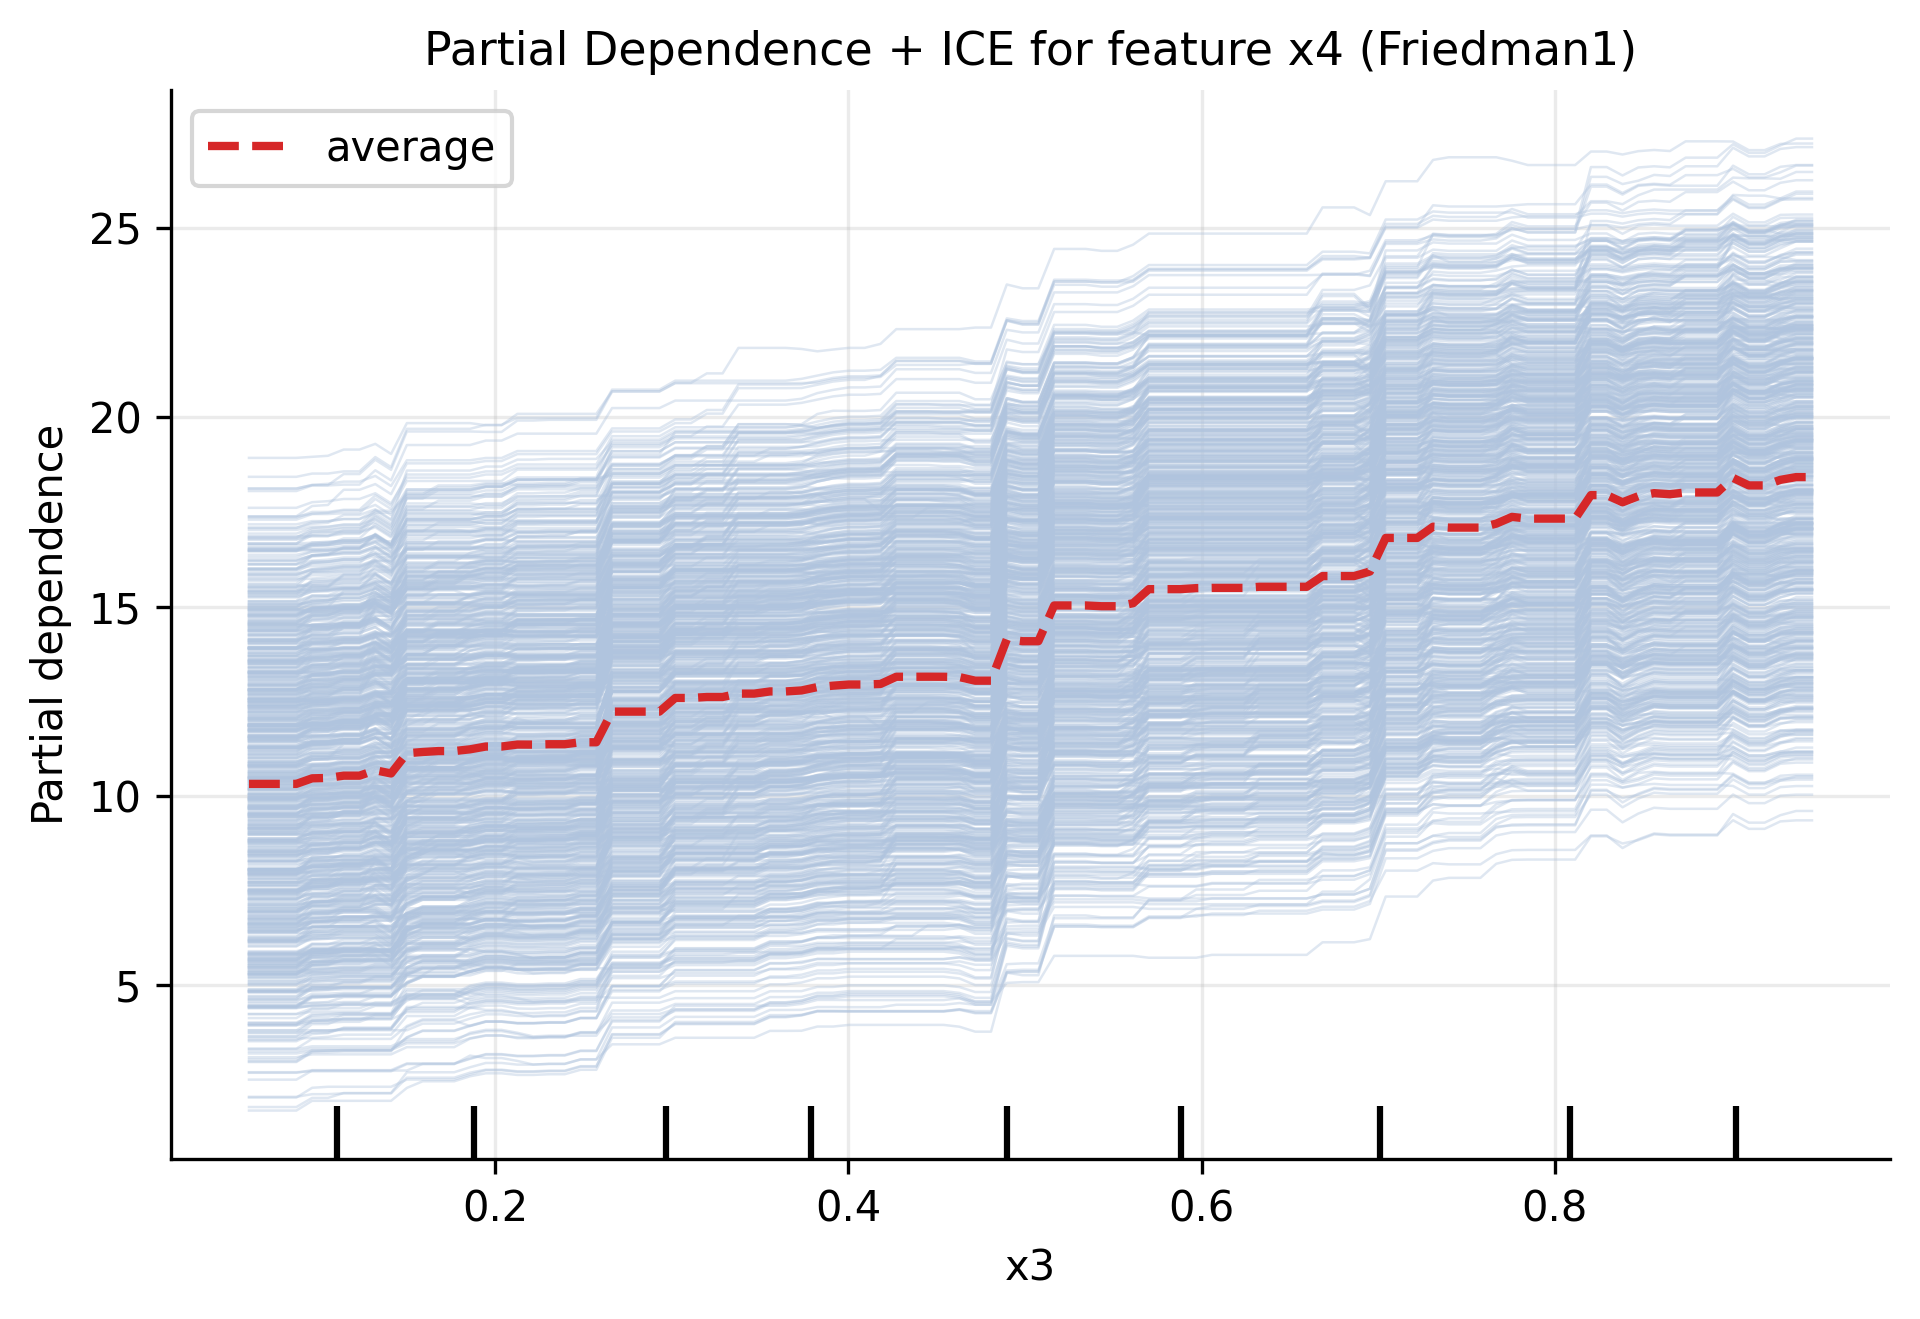
\includegraphics[width=0.85\linewidth]{figures/pdp_ice.png}
\caption{Partial Dependence (red) and Individual Conditional Expectation lines (light blue) for feature $x_4$ of a Gradient Boosting regressor on Friedman~1. The PDP is the average over all ICE curves; large ICE dispersion would signal feature interactions hidden by the PDP.}
\label{fig:pdp-ice}
\end{figure}

\subsubsection{21.1 Partial dependence}\label{211-partial-dependence}

Friedman (Annals of Statistics 2001). For a feature (or feature subset)
\(X_S\): \[
\mathrm{PDP}_S(x_S) = \mathbb{E}_{X_{\bar{S}}}[f(x_S, X_{\bar{S}})] \approx \frac{1}{n}\sum_{i=1}^{n} f(x_S, x_{\bar{S}, i}).
\] A PDP plots \(\mathrm{PDP}_S\) as a function of \(x_S\) (one curve
for one feature; a 3D surface or heatmap for two).

\textbf{Intuition}: the marginal effect of \(X_S\) on predictions,
averaged over the empirical distribution of the other features.

\subsubsection{21.2 Individual Conditional Expectation
(ICE)}\label{212-individual-conditional-expectation-ice}

Goldstein et al. (JCGS 2015). PDP without the averaging: one curve per
observation, \[
\mathrm{ICE}_S^{(i)}(x_S) = f(x_S, x_{\bar{S}, i}).
\] An ICE plot draws all \(n\) curves overlaid; the PDP is their
pointwise mean. \textbf{ICE exposes interactions and heterogeneity that
the PDP averages away} --- if the curves fan out, the effect of \(X_S\)
depends on the values of the other features.

\textbf{Centred ICE (c-ICE)}: subtract each curve\textquotesingle s
value at the leftmost grid point, so all curves start at zero. Makes
heterogeneity in \emph{changes} visible without the distraction of
different intercepts.

\subsubsection{21.3 Accumulated Local Effects
(ALE)}\label{213-accumulated-local-effects-ale}

Apley \& Zhu (JRSS-B 2020). PDP evaluates the model at
\((x_S, x_{\bar{S}, i})\) combinations that may be off the data manifold
--- the same extrapolation pathology that afflicts interventional SHAP
and PFI. ALE plots use \textbf{conditional} expectations integrated over
local windows of \(x_S\): \[
\mathrm{ALE}_S(x_S) = \int_{\min(x_S)}^{x_S} \mathbb{E}\left[\frac{\partial f(u, X_{\bar{S}})}{\partial u} \,\Big|\, X_S = u\right] du - \text{const}.
\] Empirically: bin \(X_S\), compute the average within-bin change in
\(f\) (conditioning on \(X_S\) in the bin, not marginalising),
accumulate, recentre.

\textbf{Use ALE instead of PDP when features are correlated.} ALE never
queries the model at off-manifold points.

\subsubsection{21.4 Code}\label{214-code}

\begin{lstlisting}[language=Python]
import numpy as np
from sklearn.ensemble import RandomForestRegressor
from sklearn.inspection import PartialDependenceDisplay
import matplotlib.pyplot as plt

rng = np.random.default_rng(0)
n = 500
X = rng.uniform(-2, 2, size=(n, 3))
y = X[:, 0] ** 2 - X[:, 1] + X[:, 0] * X[:, 2] + 0.2 * rng.normal(size=n)

model = RandomForestRegressor(n_estimators=200, random_state=0).fit(X, y)

# PDP + ICE for feature 0
fig, ax = plt.subplots(figsize=(6, 4))
PartialDependenceDisplay.from_estimator(model, X, features=[0], kind="both", ax=ax)
plt.tight_layout()
# For ALE use the PyALE package: ale_plot(model, X, features=[0])
\end{lstlisting}

\subsubsection{21.5 Properties}\label{215-properties}

\begin{itemize}
\tightlist
\item
  \textbf{PDP averages out interactions} --- a flat PDP does \emph{not}
  mean a feature has no effect (it may have heterogeneous effects that
  cancel on average).
\item
  \textbf{ICE reveals interactions} but is visually noisy for large
  \(n\) --- subsample.
\item
  \textbf{ALE avoids extrapolation} at the cost of slight bias when
  window sizes are too large.
\end{itemize}

\subsubsection{21.6 Pitfalls}\label{216-pitfalls}

\begin{itemize}
\tightlist
\item
  \textbf{Extrapolation} for PDP: the marginalisation
  \(\mathbb{E}_{X_{\bar{S}}}\) uses the unconditional distribution,
  generating feature combinations the model never trained on.
\item
  \textbf{Averaging hides interactions} --- always look at the ICE
  alongside.
\item
  \textbf{Computational cost} of PDP for two features simultaneously is
  \(O(n \cdot g^2)\) where \(g\) is grid resolution.
\item
  \textbf{PDP is not a causal effect} --- it shows how the
  model\textquotesingle s prediction \emph{would respond} to changing
  \(X_S\) holding the conditional distribution of other features
  fixed-at-marginal, which is not generally the same as the causal
  effect of intervening on \(X_S\).
\end{itemize}

\subsubsection{21.7 When to use}\label{217-when-to-use}

Whenever you want to \emph{see} (not just rank) a
feature\textquotesingle s effect on a model. Especially useful for
non-linear models where coefficients are unavailable. \textbf{ALE for
correlated features.} PDP + ICE for an initial diagnostic. Two-feature
PDP heatmaps to visualise pairwise interactions.

\begin{center}\rule{0.5\linewidth}{0.5pt}\end{center}

\section{Part V --- Tree-Specific and Embedded
Metrics}\label{part-v--tree-specific-and-embedded-metrics}

Tree-based models (decision trees, random forests, gradient boosting)
compute "importance" as a by-product of training. These are cheap,
ubiquitous, and frequently misinterpreted --- each carries
well-documented biases that make them poor substitutes for the
model-agnostic measures in Part IV. The same is true of the regression
coefficients in penalised linear models, which double as importance
scores by design.

\subsection{22. Gini Importance / Mean Decrease in Impurity
(MDI)}\label{22-gini-importance--mean-decrease-in-impurity-mdi}

\subsubsection{22.1 Definition}\label{221-definition}

For a single decision tree, the importance of feature \(i\) is the total
impurity reduction at all internal nodes that split on \(i\), weighted
by the fraction of training samples reaching each node: \[
\mathrm{MDI}_i = \sum_{t \in T_i} \frac{n_t}{n} \Delta i(t),
\] where \(T_i\) is the set of internal nodes splitting on feature
\(i\), \(n_t\) is the number of training samples at node \(t\), and the
impurity decrease is \[
\Delta i(t) = i(t) - \frac{n_{t_L}}{n_t} i(t_L) - \frac{n_{t_R}}{n_t} i(t_R).
\] For classification \(i(t)\) is the \textbf{Gini index}
\(1 - \sum_k p_{tk}^2\) or \textbf{entropy}
\(-\sum_k p_{tk} \log p_{tk}\); for regression it is the variance
\(\frac{1}{n_t}\sum_{x \in t}(y - \bar{y}_t)^2\).

For an ensemble (random forest, extra trees), average MDI across trees.

\subsubsection{22.2 Intuition}\label{222-intuition}

"How much does this feature reduce impurity, summed over all the times
the greedy algorithm chose to split on it, weighted by how many training
samples were affected?"

\subsubsection{22.3 Why MDI is biased --- three
reasons}\label{223-why-mdi-is-biased--three-reasons}

\begin{enumerate}
\def\labelenumi{\arabic{enumi}.}
\tightlist
\item
  \textbf{Cardinality bias.} Features with more possible split points
  (continuous, or categorical with many levels) have more chances to be
  selected greedily and tend to acquire larger MDI even when
  uninformative. Strobl et al. (BMC Bioinformatics 2007) is the
  canonical demonstration.
\item
  \textbf{Computed on training data.} MDI reflects how the trees were
  built, not whether splits generalise. A noise feature can acquire
  non-trivial MDI through overfitting in deep trees.
\item
  \textbf{Correlated features dilute each other.} Two features with
  identical signal split the MDI; if you remove one, the
  other\textquotesingle s MDI roughly doubles.
\end{enumerate}

\subsubsection{22.4 Empirical demonstration of cardinality
bias}\label{224-empirical-demonstration-of-cardinality-bias}

\begin{lstlisting}[language=Python]
import numpy as np
from sklearn.ensemble import RandomForestRegressor

rng = np.random.default_rng(0)
n = 2000
# Pure noise: a binary feature, a 10-category, and a continuous, all unrelated to y
X = np.column_stack([
    rng.integers(0, 2, n).astype(float),    # 2 levels
    rng.integers(0, 10, n).astype(float),   # 10 levels
    rng.normal(size=n),                     # continuous (many split points)
])
y = rng.normal(size=n)  # pure noise

model = RandomForestRegressor(n_estimators=500, random_state=0).fit(X, y)
print("Pure noise features; ideal MDI would be ~equal (or zero):")
for i, imp in enumerate(model.feature_importances_):
    print(f"  feature {i}: MDI = {imp:.4f}")
# The continuous feature will dominate, despite all being equally uninformative.
\end{lstlisting}

\subsubsection{22.5 Unbiased
alternatives}\label{225-unbiased-alternatives}

\begin{itemize}
\tightlist
\item
  \textbf{Conditional inference forests} (Hothorn et al. 2006;
  \texttt{party::cforest} in R) use significance-test-based splitting
  that removes the cardinality bias.
\item
  \textbf{Honest forests / unbiased MDI} (Li, Wang, Singh 2019):
  randomly subsample data for splitting vs leaf-value estimation,
  removing the in-sample-optimism bias.
\item
  \textbf{MDA (§23) and PFI (§19) on held-out data} are usually
  preferred.
\end{itemize}

\subsubsection{22.6 When to use}\label{226-when-to-use}

A cheap first look at what a forest is doing. \textbf{Always cross-check
with held-out PFI before reporting}. Never use MDI alone in a setting
that affects decisions.

\begin{center}\rule{0.5\linewidth}{0.5pt}\end{center}

\subsection{23. Mean Decrease in Accuracy
(MDA)}\label{23-mean-decrease-in-accuracy-mda}

\subsubsection{23.1 Algorithm}\label{231-algorithm}

The original Breiman (2001) random forest importance:

\begin{enumerate}
\def\labelenumi{\arabic{enumi}.}
\tightlist
\item
  For each tree \(t\) in the forest, evaluate prediction accuracy on its
  OOB sample \(O_t\).
\item
  Permute feature \(i\) across \(O_t\); re-evaluate accuracy.
\item
  The per-tree importance is the accuracy drop. MDA of feature \(i\) is
  the average drop across trees.
\end{enumerate}

\subsubsection{23.2 Relationship to PFI}\label{232-relationship-to-pfi}

MDA is permutation feature importance evaluated within each
tree\textquotesingle s OOB sample. Statistically more efficient than
computing a separate held-out PFI, because OOB samples are "free" ---
each tree saw a different bootstrap subset, and the rest serves as its
private test set.

\subsubsection{23.3 Properties}\label{233-properties}

\begin{itemize}
\tightlist
\item
  Less biased than MDI (uses held-out data via OOB).
\item
  Inherits all PFI pitfalls: correlated-feature instability,
  extrapolation, retraining sensitivity.
\item
  Specific to bagging-based ensembles (random forests, extra trees); not
  natively defined in boosting.
\end{itemize}

\subsubsection{23.4 Code}\label{234-code}

\begin{lstlisting}[language=Python]
import numpy as np
from sklearn.ensemble import RandomForestRegressor
from sklearn.datasets import make_regression
from sklearn.inspection import permutation_importance

X, y = make_regression(n_samples=1000, n_features=10, n_informative=5,
                        noise=1.0, random_state=0)
model = RandomForestRegressor(n_estimators=500, oob_score=True, random_state=0).fit(X, y)

# scikit-learn does not expose Breiman-style OOB MDA directly; use permutation_importance on a held-out set,
# or compute manually using model.estimators_ and their bootstrap indices.
# For practical purposes, the result is close to:
result = permutation_importance(model, X, y, n_repeats=20, random_state=0)
for i in range(X.shape[1]):
    print(f"feature {i}: MDA-equiv = {result.importances_mean[i]:+.4f}")
\end{lstlisting}

\subsubsection{23.5 When to use}\label{235-when-to-use}

Default importance for random forests when you don\textquotesingle t
have a separate held-out PFI run. \textbf{Prefer to MDI} in nearly all
cases.

\begin{center}\rule{0.5\linewidth}{0.5pt}\end{center}

\subsection{24. Gain, Split, and Cover Importance in Boosted
Trees}\label{24-gain-split-and-cover-importance-in-boosted-trees}

Gradient-boosted ensembles (XGBoost, LightGBM, CatBoost) report multiple
importance types:

\subsubsection{24.1 Definitions}\label{241-definitions}

\begin{itemize}
\tightlist
\item
  \textbf{Gain} (a.k.a. \emph{total gain}): sum of loss reduction
  attributable to splits on the feature, across all trees. Boosting
  analogue of MDI; typical default.
\item
  \textbf{Split} (a.k.a. \emph{weight} or \emph{frequency}): number of
  times the feature was used as a split.
\item
  \textbf{Cover} (a.k.a. \emph{sample coverage}): average number of
  training samples flowing through splits that used the feature.
\item
  \textbf{Total cover}: sum (not average) of cover.
\end{itemize}

In XGBoost: \texttt{importance\_type} ∈ \{\texttt{gain},
\texttt{weight}, \texttt{cover}, \texttt{total\_gain},
\texttt{total\_cover}\}. In LightGBM: \texttt{importance\_type} ∈
\{\texttt{gain}, \texttt{split}\}.

\subsubsection{24.2 Differences from
MDI}\label{242-differences-from-mdi}

Boosting trees are typically shallow (the \emph{weak learner} idea,
\(\text{depth} \in [3, 8]\)), so the cardinality bias of MDI is
attenuated. However:

\begin{itemize}
\tightlist
\item
  \textbf{Gain is still computed on training data} and inflates with
  noise overfitting under under-regularisation.
\item
  \textbf{Split} is the most directly comparable to "frequency of use"
  and is preferred when features have very different resolutions of
  potential split points.
\item
  \textbf{Cover} is most relevant when you care about \emph{how much of
  the data} a feature influenced.
\end{itemize}

\subsubsection{24.3 TreeSHAP as the modern
replacement}\label{243-treeshap-as-the-modern-replacement}

Lundberg et al. (2018) showed that gain importance can produce
misleading rankings under correlated features and proposed TreeSHAP as
the principled alternative. For XGBoost / LightGBM, \textbf{prefer
TreeSHAP} for any decision that matters; use gain / split / cover for
quick triage.

CatBoost is somewhat different: its native "PredictionValuesChange"
measures average change in predictions when the feature value changes;
"LossFunctionChange" ≈ permutation importance, computed efficiently.
Both are closer to PFI than to gain.

\subsubsection{24.4 Code}\label{244-code}

\begin{lstlisting}[language=Python]
# pip install xgboost
import xgboost as xgb
import numpy as np

rng = np.random.default_rng(0)
n, p = 1000, 6
X = rng.normal(size=(n, p))
y = 2 * X[:, 0] + X[:, 1] ** 2 + 0.3 * rng.normal(size=n)

model = xgb.XGBRegressor(n_estimators=200, max_depth=4).fit(X, y)

for itype in ["gain", "weight", "cover", "total_gain", "total_cover"]:
    scores = model.get_booster().get_score(importance_type=itype)
    print(f"\n{itype}:")
    for k, v in sorted(scores.items(), key=lambda kv: -kv[1]):
        print(f"  {k}: {v:.4f}")
\end{lstlisting}

\subsubsection{24.5 When to use}\label{245-when-to-use}

\begin{itemize}
\tightlist
\item
  \textbf{Gain}: quick training-time importance for a fitted booster;
  sanity check.
\item
  \textbf{Split}: when you care about how often a feature is consulted
  (e.g. for feature pruning decisions).
\item
  \textbf{Cover}: rarely the right answer; useful for diagnosis.
\item
  For anything decision-relevant: \textbf{TreeSHAP}.
\end{itemize}

\begin{center}\rule{0.5\linewidth}{0.5pt}\end{center}

\subsection{25. LASSO and Ridge Coefficients as
Importance}\label{25-lasso-and-ridge-coefficients-as-importance}

\subsubsection{25.1 Definitions}\label{251-definitions}

\textbf{LASSO} (\(L_1\) regularised regression; Tibshirani JRSS-B 1996):
\[
\hat{\beta}_{\mathrm{LASSO}} = \arg\min_\beta \frac{1}{2n}\|\mathbf{y} - \mathbf{X}\beta\|_2^2 + \lambda \|\beta\|_1.
\]

\textbf{Ridge} (\(L_2\); Hoerl \& Kennard Technometrics 1970): \[
\hat{\beta}_{\mathrm{Ridge}} = \arg\min_\beta \frac{1}{2n}\|\mathbf{y} - \mathbf{X}\beta\|_2^2 + \lambda \|\beta\|_2^2.
\]

\textbf{Elastic Net} (Zou \& Hastie JRSS-B 2005): combines both, \[
\hat{\beta}_{\mathrm{EN}} = \arg\min_\beta \frac{1}{2n}\|\mathbf{y} - \mathbf{X}\beta\|_2^2 + \lambda_1 \|\beta\|_1 + \lambda_2 \|\beta\|_2^2.
\]

\subsubsection{\texorpdfstring{25.2 The geometry of \(L_1\) vs
\(L_2\)}{25.2 The geometry of L\_1 vs L\_2}}\label{252-the-geometry-of-l_1-vs-l_2}

The \(L_1\) unit ball has \textbf{corners on the axes}; the \(L_2\) unit
ball is round. As the OLS solution shrinks under penalty, the contact
point with the \(L_1\) ball tends to lie on a corner (a coordinate
plane), making some coefficients exactly zero. The \(L_2\) contact point
is generically interior, so all coefficients shrink toward zero but none
reach it. This geometric intuition is the cleanest explanation of why
LASSO performs feature selection and Ridge does not.

\subsubsection{25.3 Closed-form Ridge
solution}\label{253-closed-form-ridge-solution}

\[
\hat{\beta}_{\mathrm{Ridge}} = (\mathbf{X}^\top \mathbf{X} + n\lambda I)^{-1} \mathbf{X}^\top \mathbf{y}.
\] Always invertible (adding \(n\lambda I\) regularises the Gram
matrix). LASSO has no closed form; coordinate descent (Friedman et al.
2007) is the dominant solver and what \texttt{glmnet} and
\texttt{sklearn} use under the hood.

\subsubsection{25.4 Critical
preprocessing}\label{254-critical-preprocessing}

\begin{itemize}
\tightlist
\item
  \textbf{Standardise features} (mean 0, unit variance). Otherwise the
  penalty applies unequally --- large-scale features look spuriously
  unimportant.
\item
  \textbf{Tune \(\lambda\) by cross-validation} (\texttt{LassoCV},
  \texttt{RidgeCV}, \texttt{ElasticNetCV}). Importance rankings depend
  on \(\lambda\).
\item
  \textbf{Centre \(\mathbf{y}\)} (or include an unpenalised intercept;
  the standard \texttt{sklearn} and \texttt{glmnet} interfaces do this
  automatically).
\end{itemize}

\subsubsection{25.5 Stability under correlated
features}\label{255-stability-under-correlated-features}

LASSO is \emph{known} to be unstable under multicollinearity --- it
tends to pick one feature from each correlated group and zero out the
rest, with the choice sensitive to the random sample. Three responses:

\begin{itemize}
\tightlist
\item
  \textbf{Elastic Net}: the \(L_2\) component groups correlated features
  (they survive together or perish together), recommended whenever you
  expect correlated predictors.
\item
  \textbf{Stability Selection} (Meinshausen \& Bühlmann JRSS-B 2010):
  rerun LASSO on bootstrap subsamples; report features selected in a
  high fraction of runs.
\item
  \textbf{Adaptive LASSO} (Zou JASA 2006): reweight the penalty by an
  initial estimate (\(w_i \propto 1/|\tilde{\beta}_i|^\gamma\)), giving
  oracle consistency properties.
\end{itemize}

\subsubsection{25.6 Post-selection
inference}\label{256-post-selection-inference}

LASSO coefficients are \textbf{biased toward zero} by construction; the
usual OLS \(t\)-tests on the selected features are \emph{invalid} (they
ignore the selection step). Two principled solutions:

\begin{itemize}
\tightlist
\item
  \textbf{LASSO + OLS refit}: use LASSO to select features, then refit
  by OLS on selected features for unbiased estimates. Simple, widely
  used, but inferentially imperfect.
\item
  \textbf{Selective inference} (Lee et al. 2016; Tibshirani et al.
  2016): build confidence intervals that condition on the selection
  event. Implemented in the R \texttt{selectiveInference} package; rare
  in Python.
\end{itemize}

\subsubsection{25.7 Code}\label{257-code}

\begin{lstlisting}[language=Python]
import numpy as np
from sklearn.linear_model import LassoCV, RidgeCV, ElasticNetCV
from sklearn.preprocessing import StandardScaler
from sklearn.pipeline import make_pipeline

rng = np.random.default_rng(0)
n, p = 200, 20
X = rng.normal(size=(n, p))
true_beta = np.zeros(p); true_beta[:5] = [2, -1.5, 1, -0.5, 0.8]  # only first 5 matter
y = X @ true_beta + 0.5 * rng.normal(size=n)

# Standardise + cross-validated LASSO
lasso = make_pipeline(StandardScaler(), LassoCV(cv=5, random_state=0)).fit(X, y)
beta = lasso[-1].coef_

print("LASSO coefficients (showing non-zero):")
for i, b in enumerate(beta):
    marker = "  <- true signal" if i < 5 else ""
    if abs(b) > 1e-6:
        print(f"  beta[{i}] = {b:+.3f}{marker}")
print(f"\nNumber of selected features: {(np.abs(beta) > 1e-6).sum()}")
print(f"Chosen lambda: {lasso[-1].alpha_:.4f}")
\end{lstlisting}

\subsubsection{25.8 Other uses}\label{258-other-uses}

\begin{itemize}
\tightlist
\item
  \textbf{Logistic LASSO} for classification --- same penalty,
  coefficients on the log-odds scale.
\item
  \textbf{Group LASSO} (Yuan \& Lin 2006) for selecting whole groups of
  features (e.g. all dummies for a categorical variable).
\item
  \textbf{Sparse logistic regression} is the standard tool for
  high-dimensional binary screening (genomics, NLP).
\end{itemize}

\subsubsection{25.9 Pitfalls}\label{259-pitfalls}

\begin{itemize}
\tightlist
\item
  \textbf{Coefficients are only meaningful after standardisation};
  otherwise their magnitudes mix penalty effects with scale.
\item
  \textbf{Sign is interpretable}; magnitude is comparable across
  features \emph{only} after standardisation.
\item
  \textbf{Highly biased toward zero by construction} --- for unbiased
  estimates use the LASSO selection as a \emph{first step} followed by
  OLS on the selected features.
\item
  \textbf{No interactions} in vanilla LASSO; include explicit
  interaction terms or use tree-based methods.
\item
  \textbf{High-correlation pairs} behave unpredictably without Elastic
  Net or Stability Selection.
\end{itemize}

\subsubsection{25.10 When to use}\label{2510-when-to-use}

Linear (or generalised linear) modelling with many features;
high-dimensional problems where \(p > n\); cases where sparsity is
intrinsic to the scientific story; feature pre-screening before fitting
a non-linear model.

\begin{center}\rule{0.5\linewidth}{0.5pt}\end{center}

\section{Cross-Cutting Themes}\label{cross-cutting-themes}

\subsection{Choosing a Measure: A Decision
Tree}\label{choosing-a-measure-a-decision-tree}

A condensed walk-through:

\begin{enumerate}
\def\labelenumi{\arabic{enumi}.}
\item
  \textbf{What are you measuring --- raw variables or a fitted model?}

  \begin{itemize}
  \tightlist
  \item
    Raw variables → Parts I, II, III.
  \item
    Fitted model → Parts IV, V.
  \end{itemize}
\item
  \textbf{For raw variables, what are the data types?}

  \begin{itemize}
  \tightlist
  \item
    Continuous--continuous → Pearson (linear), Spearman (monotone), dCor
    / HSIC / MI (general).
  \item
    Continuous--ordinal → Spearman, Kendall; polychoric if you believe a
    latent normal.
  \item
    Continuous--binary → Point-biserial.
  \item
    Binary--binary → \(\phi\); tetrachoric if you believe latent normal.
  \item
    Categorical--categorical → Cramér\textquotesingle s \(V\); MI / NMI.
  \item
    Multivariate--multivariate → dCor, HSIC, KCCA.
  \item
    Time series with direction → Transfer entropy.
  \item
    Conditional dependence → Partial correlation (linear), CMI,
    conditional HSIC, conditional Chatterjee.
  \end{itemize}
\item
  \textbf{How non-linear do you expect the relationship?}

  \begin{itemize}
  \tightlist
  \item
    Linear → Pearson.
  \item
    Monotone → Spearman, Kendall.
  \item
    Functional non-monotone → Chatterjee \(\xi\), dCor, HSIC, MI.
  \item
    Anything → MI, dCor, HSIC.
  \end{itemize}
\item
  \textbf{Do you need a hypothesis test?}

  \begin{itemize}
  \tightlist
  \item
    Pearson, Spearman, Kendall, \(\phi\), point-biserial,
    Cramér\textquotesingle s \(V\) --- closed-form tests.
  \item
    Chatterjee \(\xi\) --- closed-form asymptotic normal.
  \item
    dCor, HSIC, MI, MIC, TE, CMI --- permutation tests are the gold
    standard; gamma approximations for HSIC.
  \end{itemize}
\item
  \textbf{For model feature importance, what kind of model and what
  question?}

  \begin{itemize}
  \tightlist
  \item
    Tree ensemble + global ranking → TreeSHAP (preferred), or MDI / Gain
    (cheap).
  \item
    Any model + global ranking → PFI on held-out data.
  \item
    Any model + per-prediction explanation → SHAP.
  \item
    Per-prediction explanation of image / text → LIME.
  \item
    Visualising a feature\textquotesingle s effect → PDP + ICE, or ALE
    for correlated features.
  \item
    Linear / GLM with sparsity → LASSO coefficients (after
    standardisation).
  \end{itemize}
\end{enumerate}

\subsection{Significance, Permutation Tests, and Confidence
Intervals}\label{significance-permutation-tests-and-confidence-intervals}

Every dependence measure in this guide can be turned into a hypothesis
test of \(H_0: X \perp Y\). Two routes:

\begin{itemize}
\tightlist
\item
  \textbf{Asymptotic null distributions.} Available for Pearson,
  Spearman, Kendall, \(\phi\), point-biserial, Cramér\textquotesingle s
  \(V\), Chatterjee\textquotesingle s \(\xi\), and (with care) HSIC and
  dCor. Use when \(n\) is large and assumptions are met.
\item
  \textbf{Permutation tests.} Compute \(D\) on the original data;
  randomly permute one variable many times and recompute \(D\) on each
  permutation; report the fraction of permutations exceeding the
  observed value as the \(p\)-value. Exact under \(H_0\) up to Monte
  Carlo error; the universal fallback.
\end{itemize}

For \textbf{confidence intervals}, the \textbf{bootstrap} is universal:
resample with replacement, recompute, report percentiles. For Pearson
and Spearman, Fisher\textquotesingle s \(z\)-transform gives narrower
CIs under normality.

Two corner cases:

\begin{itemize}
\tightlist
\item
  The bootstrap can be \textbf{biased downward} for measures that are
  non-negative and bounded above (MI, dCor, HSIC); the \textbf{BCa}
  (bias-corrected and accelerated) bootstrap is preferred.
\item
  For \textbf{time series}, ordinary permutation / bootstrap destroys
  temporal structure and is \textbf{invalid}. Use the \textbf{block
  bootstrap} with block length matched to the autocorrelation time
  scale.
\end{itemize}

\subsection{Multiple Testing and the Garden of Forking
Paths}\label{multiple-testing-and-the-garden-of-forking-paths}

Computing \(p\)-values for every pair of features in a 100-feature
dataset gives 4\{,\}950 tests --- at \(\alpha = 0.05\),
\textasciitilde250 will fire even if every pair is independent. Two
corrections:

\begin{itemize}
\tightlist
\item
  \textbf{Bonferroni}: \(\alpha / m\). Simple, conservative, controls
  \textbf{family-wise error rate (FWER)}.
\item
  \textbf{Benjamini--Hochberg (BH)}: sort \(p\)-values; reject
  \(p_{(k)}\) if \(p_{(k)} \leq k\alpha/m\) for some \(k\). Controls
  \textbf{false discovery rate (FDR)} --- the expected proportion of
  false positives among the rejections. More powerful than Bonferroni;
  the standard default for screening.
\end{itemize}

The deeper, harder problem is the \textbf{garden of forking paths}
(Gelman \& Loken 2013): even a single measure, computed across many
plausible analytical choices (transformations, outlier rules,
subsamples, model variants), implicitly searches a space of hypotheses
without correction. Pre-registration, hold-out validation, and an honest
accounting of how many models were tried are the only real defences.

\subsection{Correlation, Causation, and
Confounders}\label{correlation-causation-and-confounders}

No measure in this document --- not Pearson, not dCor, not SHAP, not
Chatterjee\textquotesingle s \(\xi\) --- distinguishes correlation from
causation on its own. They all summarise \emph{statistical} dependence
in the observed joint distribution. Common causes (confounders) produce
association without causation; selection effects produce association
where none exists in the underlying population; measurement error
attenuates association even when causation is real.

The three main routes to causal claims:

\begin{enumerate}
\def\labelenumi{\arabic{enumi}.}
\tightlist
\item
  \textbf{Randomised experiments.} The gold standard. Random assignment
  breaks confounding by construction.
\item
  \textbf{DAG-based observational reasoning} (Pearl, Imbens \& Rubin,
  Hernán \& Robins). Posit a causal DAG; use the back-door, front-door,
  or instrumental-variable criteria; estimate effects with the
  appropriate adjustment set.
\item
  \textbf{Natural experiments and quasi-experiments}: regression
  discontinuity, difference-in-differences, instrumental variables.
\end{enumerate}

The dependence measures in this guide are inputs to step 2 --- they
identify candidate associations and CI relations --- but they do not
themselves produce causal claims. SHAP attributing high importance to a
feature does \textbf{not} mean intervening on that feature changes the
outcome. Conversely, a causally important feature can have small SHAP
under a model that uses a proxy.

\subsection{Pitfalls Common to All
Metrics}\label{pitfalls-common-to-all-metrics}

A short, brutal checklist:

\begin{itemize}
\tightlist
\item
  \textbf{Sample size dominates.} Most measures are upward biased at
  small \(n\) --- particularly MI, MIC, dCor, HSIC. Report estimators
  with sampling distributions, not as points.
\item
  \textbf{Outliers distort.} Pearson is the worst offender; rank-based
  and information-theoretic measures are more robust but not immune.
\item
  \textbf{Discretisation choices matter.} MI, MIC, transfer entropy
  depend on binning or kernel bandwidth.
\item
  \textbf{High dimensions are hard.} \(n / d\) ratios below 10 make
  non-parametric estimators very noisy.
\item
  \textbf{Stationarity for time series.} Without it, transfer entropy,
  autocorrelation, and most everything else are meaningless.
\item
  \textbf{Correlated features confuse importance.} SHAP, PFI, MDI, gain
  --- all of them split credit between correlated features in ways that
  are hard to interpret.
\item
  \textbf{Training vs held-out data.} Importance measures computed on
  training data measure memorisation, not generalisation.
\item
  \textbf{A single number is rarely enough.} Always pair a coefficient
  with a plot. Anscombe\textquotesingle s quartet exists for a reason.
\end{itemize}

\begin{center}\rule{0.5\linewidth}{0.5pt}\end{center}

\section{Common Confusions and How to Resolve
Them}\label{common-confusions-and-how-to-resolve-them}

The pairings below are the most-frequent confusions in practice. Each
gets a one-paragraph resolution.

\subsection{"Pearson vs covariance"}\label{pearson-vs-covariance}

Covariance is unbounded and scale-dependent; Pearson is the scale-free
version. \(r = \mathrm{Cov}(X, Y) / (\sigma_X \sigma_Y)\). Two datasets
with covariance 5 and 50 may have identical Pearson if the marginal
variances scale accordingly. \textbf{Report Pearson unless you
specifically need the unit-bearing covariance} (e.g., for portfolio
variance calculations where covariance contributes directly to
\(\sigma_p^2 = \sum_{ij} w_i w_j \sigma_{ij}\)).

\subsection{"Spearman vs Pearson --- which to default
to?"}\label{spearman-vs-pearson--which-to-default-to}

If you don\textquotesingle t know the relationship shape, \textbf{report
both}. A large \(r\) with a similar \(\rho_S\) confirms linearity; a
small \(r\) with a large \(\rho_S\) signals monotonic non-linearity; a
small \(\rho_S\) with a large dCor signals non-monotonic dependence.
Spearman is more robust by default; Pearson is the appropriate target
when downstream methods (PCA, OLS, multivariate normal models) assume
linearity.

\subsection{"MI vs correlation --- interpretive
equivalence?"}\label{mi-vs-correlation--interpretive-equivalence}

For jointly normal \((X, Y)\) with Pearson correlation \(\rho\):
\(I(X; Y) = -\tfrac{1}{2}\log(1 - \rho^2)\). This is one of the few
cases where MI and correlation map exactly. Outside normality,
\textbf{MI captures dependences that correlation does not} (the
\(Y = X^2\) counterexample) and \textbf{correlation captures direction
information that MI discards}. The two are complementary, not
interchangeable.

\subsection{"dCor vs HSIC"}\label{dcor-vs-hsic}

Functionally near-equivalent: both are non-linear, both characterise
independence, both are \(O(n^2)\), both use permutation tests. dCor is
parameter-free (distance is the only choice); HSIC requires kernel +
bandwidth. \textbf{Default to dCor} for raw screening; switch to HSIC
when you need kernel flexibility (e.g., to compare representations via
CKA) or when the random-feature approximations make the large-\(n\) case
tractable.

\subsection{"SHAP vs PFI"}\label{shap-vs-pfi}

Both are model-agnostic global importance scores, both popular, often
producing similar rankings. Differences:

\begin{itemize}
\tightlist
\item
  \textbf{SHAP}: per-prediction first, aggregate second; principled
  (Shapley axioms); reveals direction (positive/negative effect); slow
  without TreeSHAP.
\item
  \textbf{PFI}: aggregate only; not axiomatic; signless (magnitude of
  score change); fast.
\end{itemize}

Use SHAP when individual explanations matter or when direction is
informative. Use PFI for a quick, model-agnostic global ranking.
\textbf{Do not average their rankings naively} --- they answer slightly
different questions.

\subsection{"MDI vs PFI vs SHAP for tree
ensembles"}\label{mdi-vs-pfi-vs-shap-for-tree-ensembles}

\begin{itemize}
\tightlist
\item
  \textbf{MDI} is cheapest, computed during training, but biased toward
  high-cardinality features.
\item
  \textbf{PFI on held-out data} removes the bias and reflects
  generalisation, but suffers correlated-feature instability.
\item
  \textbf{TreeSHAP} is the principled gold standard; exact, fast for
  trees, axiomatic, reveals direction.
\end{itemize}

For research or production decisions, prefer \textbf{TreeSHAP}. MDI is
for triage.

\subsection{"LIME vs SHAP"}\label{lime-vs-shap}

LIME approximates the model locally with a sparse linear surrogate
fitted on perturbed samples. SHAP computes Shapley values of features,
providing exact additive decomposition. \textbf{SHAP can be derived as a
special-case linear regression on coalitions with specific weights} (the
"kernel SHAP" reformulation), placing LIME and SHAP in the same family
--- but LIME\textquotesingle s kernel and sampling distribution
generally fail to recover the Shapley axioms. Use SHAP when axiomatic
guarantees matter.

\subsection{"Granger causality vs transfer
entropy"}\label{granger-causality-vs-transfer-entropy}

For jointly Gaussian linear stationary processes, transfer entropy is
monotone in the Granger \(F\)-statistic. \textbf{TE is the nonlinear,
non-parametric generalisation}. Use Granger when you have a fitted
linear VAR you trust; use TE when you suspect non-linear dynamics, but
be aware that TE needs substantially more data (\(n \gtrsim 10^4\)) for
reliable estimates.

\subsection{"Partial correlation vs
CMI"}\label{partial-correlation-vs-cmi}

Partial correlation \(r_{XY \cdot Z}\) removes the \textbf{linear}
effect of \(Z\) before computing Pearson on the residuals; CMI removes
the \textbf{full statistical} effect of \(Z\). They agree under joint
normality and diverge under non-linearity. \textbf{Use partial
correlation for linear-Gaussian intuition; CMI for general
causal-discovery contexts.}

\subsection{\texorpdfstring{"Correlation between binary variables ---
should I use \(\phi\) or the odds
ratio?"}{"Correlation between binary variables --- should I use \textbackslash phi or the odds ratio?"}}\label{correlation-between-binary-variables--should-i-use-phi-or-the-odds-ratio}

\(\phi\) is symmetric, bounded in \([-1, 1]\), and is exactly Pearson on
the 0/1 codings --- but its maximum depends on the marginals. OR is
invariant to row/column rescaling and to the sampling design
(prospective vs retrospective), making it the standard in epidemiology.
\textbf{Report both for \(2 \times 2\) tables}: \(\phi\) as effect-size
summary, OR for design-invariant inference.

\subsection{"Adjusted Rand Index vs Adjusted Mutual Information for
clustering
comparison"}\label{adjusted-rand-index-vs-adjusted-mutual-information-for-clustering-comparison}

ARI is pair-counting; AMI is information-theoretic. Both correct for
chance. ARI tends to penalise differences in cluster shape more harshly;
AMI penalises information loss more. In a horse race they usually agree;
when they don\textquotesingle t, the difference reveals where the
partitions diverge. \textbf{Vinh, Epps \& Bailey (2010) recommend AMI}
when clusters are highly unbalanced; \textbf{ARI} when they are roughly
balanced.

\subsection{"Why does my training-set PFI show high importance for noise
features?"}\label{why-does-my-training-set-pfi-show-high-importance-for-noise-features}

Because PFI on training data measures memorisation: a tree that
memorised noise sees its training accuracy drop when the noise is
shuffled. \textbf{Always evaluate PFI on held-out data}. The same logic
explains why MDI of pure-noise high-cardinality features can be
substantial --- both are training-time signals.

\subsection{"Why don\textquotesingle t my SHAP values sum to the
prediction?"}\label{why-dont-my-shap-values-sum-to-the-prediction}

They should --- exactly. If they don\textquotesingle t, check:

\begin{enumerate}
\def\labelenumi{\arabic{enumi}.}
\tightlist
\item
  \textbf{Baseline expectation}: the decomposition is
  \(f(\mathbf{x}) = \mathbb{E}[f(\mathbf{X})] + \sum_i \phi_i\). Is
  \texttt{explainer.expected\_value} defined on the same scale as
  \texttt{model.predict()}?
\item
  \textbf{Sampling estimator}: KernelSHAP with too few samples produces
  noisy attributions that don\textquotesingle t sum exactly. Increase
  \texttt{nsamples}.
\item
  \textbf{Multiclass models}: SHAP returns one value per class; the
  per-class decomposition holds, but you must pick a class.
\item
  \textbf{Log-odds vs probability}: tree classifiers return
  probabilities, but TreeSHAP may operate on margins. Use
  \texttt{model\_output="probability"} or convert manually.
\end{enumerate}

\begin{center}\rule{0.5\linewidth}{0.5pt}\end{center}

\section{Glossary}\label{glossary}

A one-line definition for every term used in the guide that might
require a refresher. Bold terms cross-reference defining sections.

\begin{itemize}
\tightlist
\item
  \textbf{AMI} --- \emph{Adjusted Mutual Information}. NMI with
  chance-correction. §10.
\item
  \textbf{Affine invariance} --- invariance under \(X \mapsto aX + b\).
\item
  \textbf{ALE} --- \emph{Accumulated Local Effects}. PDP variant that
  avoids extrapolation under feature correlation. §21.
\item
  \textbf{Asymptotic normality} --- convergence of a properly scaled
  statistic to a normal distribution as \(n \to \infty\).
\item
  \textbf{BCa bootstrap} --- \emph{Bias-Corrected and accelerated
  bootstrap}. Improved bootstrap CI for skewed sampling distributions.
\item
  \textbf{Bernoulli distribution} --- random variable taking value 1
  with probability \(p\), 0 otherwise.
\item
  \textbf{Bias (estimator)} --- \(\mathbb{E}[\hat{\theta}] - \theta\).
\item
  \textbf{Bootstrap} --- resampling with replacement to approximate the
  sampling distribution of an estimator. P6.
\item
  \textbf{Brownian motion} --- continuous-time stochastic process with
  independent Gaussian increments. §14.
\item
  \textbf{CCA} --- \emph{Canonical Correlation Analysis}. Finds linear
  combinations of two random vectors with maximum correlation. §15.
\item
  \textbf{Characteristic function} ---
  \(\varphi_X(t) = \mathbb{E}[e^{itX}]\). P3.
\item
  \textbf{Characteristic kernel} --- kernel whose mean embedding is
  injective in the underlying distribution. P4.
\item
  \textbf{CKA} --- \emph{Centered Kernel Alignment}. Cosine version of
  HSIC. §16.
\item
  \textbf{CMI} --- \emph{Conditional Mutual Information}. §12.
\item
  \textbf{Concordant pair} --- \((x_i, y_i), (x_j, y_j)\) such that
  \((x_i - x_j)(y_i - y_j) > 0\). §3.
\item
  \textbf{Conditional independence} --- \(X \perp Y \mid Z\), meaning
  \(p_{XY \mid Z} = p_{X \mid Z} p_{Y \mid Z}\).
\item
  \textbf{Confounder} --- a variable that causally influences both
  treatment and outcome, producing spurious association.
\item
  \textbf{Copula} --- a CDF on \([0, 1]^d\) with uniform marginals,
  encoding the dependence structure separated from marginals. P7.
\item
  \textbf{Cramér\textquotesingle s \(V\)} --- categorical-categorical
  association measure based on \(\chi^2\). §6.
\item
  \textbf{Cross-covariance operator} --- operator
  \(\Sigma_{XY}: \mathcal{H}_Y \to \mathcal{H}_X\) such that
  \(\mathrm{Cov}(f(X), g(Y)) = \langle f, \Sigma_{XY} g \rangle\). §16.
\item
  \textbf{dCor} --- \emph{distance correlation}. §13.
\item
  \textbf{DAG} --- \emph{directed acyclic graph}. Used in causal
  inference. P8.
\item
  \textbf{Doubly centred matrix} --- matrix with both row and column
  means subtracted (plus the grand mean). §13.
\item
  \textbf{Eigenvalue problem} --- finding \((\lambda, v)\) with
  \(Av = \lambda v\).
\item
  \textbf{Elastic Net} --- \(L_1 + L_2\) regularised regression. §25.
\item
  \textbf{Entropy (Shannon)} --- \(H(X) = -\sum p(x) \log p(x)\). P2.
\item
  \textbf{Equitability} --- proposed property of MIC: equally noisy
  relationships should receive equal scores. §9.
\item
  \textbf{Feature map (kernel)} --- function
  \(\phi: \mathcal{X} \to \mathcal{H}\) embedding inputs into an RKHS.
  P4.
\item
  \textbf{Fisher\textquotesingle s \(z\)-transform} ---
  \(z = \operatorname{arctanh}(r)\), used to stabilise the variance of
  Pearson\textquotesingle s \(r\). §1.
\item
  \textbf{Functional dependence} --- \(Y\) is a measurable function of
  \(X\). §17.
\item
  \textbf{Gain importance} --- sum of loss reductions attributable to
  splits on a feature in boosted trees. §24.
\item
  \textbf{Gaussian process} --- collection of random variables, any
  finite subset of which is jointly Gaussian.
\item
  \textbf{Gini index} --- impurity measure \(1 - \sum_k p_k^2\). §22.
\item
  \textbf{Granger causality} --- \(X\) Granger-causes \(Y\) if past of
  \(X\) improves prediction of \(Y\) beyond past of \(Y\). P8, §11.
\item
  \textbf{HSIC} --- \emph{Hilbert--Schmidt Independence Criterion}. §16.
\item
  \textbf{ICE} --- \emph{Individual Conditional Expectation}. PDP
  without averaging. §21.
\item
  \textbf{Independence} --- \(X \perp Y\) means \(p_{XY} = p_X p_Y\).
\item
  \textbf{Interventional vs observational SHAP} --- choice of value
  function in SHAP; one breaks feature correlations, the other respects
  them. §18.
\item
  \textbf{Invariance} --- preservation under transformation. Pearson
  under affine, Spearman under monotone, MI under bijective.
\item
  \textbf{Jackknife} --- leave-one-out resampling. P6.
\item
  \textbf{KCCA} --- \emph{Kernel CCA}. §15.
\item
  \textbf{Kendall\textquotesingle s \(\tau\)} --- rank correlation based
  on concordant / discordant pairs. §3.
\item
  \textbf{Kernel} --- symmetric positive-definite function
  \(k: \mathcal{X} \times \mathcal{X} \to \mathbb{R}\). P4.
\item
  \textbf{KL divergence} ---
  \(D_{\mathrm{KL}}(p \| q) = \sum p \log(p/q)\). P2.
\item
  \textbf{KSG estimator} --- Kraskov--Stögbauer--Grassberger kNN-based
  MI estimator. §8.
\item
  \textbf{LASSO} --- \(L_1\) regularised regression. §25.
\item
  \textbf{Latent variable} --- unobserved variable inferred from
  observed indicators (e.g. tetrachoric model). §7.
\item
  \textbf{LIME} --- \emph{Local Interpretable Model-agnostic
  Explanations}. §20.
\item
  \textbf{Linear-Gaussian} --- assumption that variables are linearly
  related with Gaussian noise.
\item
  \textbf{MAD} --- \emph{Median Absolute Deviation}. Robust scale
  estimate.
\item
  \textbf{Marginal distribution} --- distribution of a single variable
  from a joint, obtained by integrating out the others.
\item
  \textbf{MDA} --- \emph{Mean Decrease in Accuracy}. §23.
\item
  \textbf{MDI} --- \emph{Mean Decrease in Impurity}. §22.
\item
  \textbf{MIC} --- \emph{Maximal Information Coefficient}. §9.
\item
  \textbf{MI} --- \emph{Mutual Information}. §8.
\item
  \textbf{Monotone transformation} --- strictly increasing (or strictly
  decreasing) function.
\item
  \textbf{Multicollinearity} --- high correlation among predictors in a
  regression.
\item
  \textbf{NMI} --- \emph{Normalized Mutual Information}. §10.
\item
  \textbf{Odds ratio} --- \(\mathrm{OR} = (ad)/(bc)\) in a
  \(2 \times 2\) table. §5.
\item
  \textbf{OLS} --- \emph{Ordinary Least Squares}. Linear regression by
  minimising squared residuals.
\item
  \textbf{Out-of-bag (OOB)} --- in a bootstrapped tree, the samples
  \emph{not} used to build that tree; provides a free held-out set. §23.
\item
  \textbf{PDP} --- \emph{Partial Dependence Plot}. §21.
\item
  \textbf{Permutation test} --- hypothesis test by shuffling labels. P6.
\item
  \textbf{PFI} --- \emph{Permutation Feature Importance}. §19.
\item
  \textbf{\(\phi\) coefficient} --- Pearson on a \(2 \times 2\) table.
  §5.
\item
  \textbf{PMF / PDF / CDF} --- probability mass / density / cumulative
  distribution function.
\item
  \textbf{Point-biserial} --- Pearson with one binary variable. §4.
\item
  \textbf{Polychoric correlation} --- latent-normal correlation
  estimated from ordinal data. §7.
\item
  \textbf{Power (statistical)} --- \(1 - P(\text{type II error})\);
  probability of rejecting \(H_0\) when it is false.
\item
  \textbf{Probit transform} --- \(\Phi^{-1}(p)\).
\item
  \textbf{Ranks} --- order statistic positions of observations.
\item
  \textbf{RBF kernel} --- \(k(x, y) = \exp(-\|x - y\|^2 / 2\sigma^2)\).
\item
  \textbf{Reproducing kernel Hilbert space (RKHS)} --- Hilbert space of
  functions in which evaluation is a continuous linear functional. P4.
\item
  \textbf{Ridge} --- \(L_2\) regularised regression. §25.
\item
  \textbf{SHAP} --- \emph{SHapley Additive exPlanations}. §18.
\item
  \textbf{Shapley value} --- unique fair-allocation rule from
  cooperative game theory. P9, §18.
\item
  \textbf{Spearman\textquotesingle s \(\rho\)} --- Pearson applied to
  ranks. §2.
\item
  \textbf{Stationarity} --- distributional invariance under time shifts.
\item
  \textbf{TE} --- \emph{Transfer Entropy}. §11.
\item
  \textbf{Tetrachoric correlation} --- polychoric specialised to
  \(2 \times 2\) tables. §7.
\item
  \textbf{TreeSHAP} --- polynomial-time exact SHAP for tree ensembles.
  §18.
\item
  \textbf{U-statistic} --- unbiased estimator written as an average over
  \(k\)-tuples. P5.
\item
  \textbf{Variational bound (MI)} --- neural-network-trained lower bound
  on MI (MINE, InfoNCE, NWJ). §8.
\end{itemize}

\begin{center}\rule{0.5\linewidth}{0.5pt}\end{center}

\section{Appendix A --- Reference Implementations and
Libraries}\label{appendix-a--reference-implementations-and-libraries}

\subsection{Python}\label{python}

{\def\LTcaptype{none} % do not increment counter
\begin{longtable}[]{@{}ll@{}}
\toprule\noalign{}
Measure & Recommended library / call \\
\midrule\noalign{}
\endhead
\bottomrule\noalign{}
\endlastfoot
Pearson, Spearman, Kendall &
\texttt{scipy.stats.\{pearsonr,\ spearmanr,\ kendalltau\}};
\texttt{pandas.DataFrame.corr} \\
Point-biserial, \(\phi\) & \texttt{scipy.stats.pointbiserialr}; Pearson
on 0/1 codings \\
Cramér\textquotesingle s \(V\) &
\texttt{scipy.stats.contingency.association(method=\textquotesingle{}cramer\textquotesingle{})}
or manually via \texttt{chi2\_contingency} \\
Tetrachoric / Polychoric &
\texttt{factor\_analyzer.utils.polychoric\_correlation};
\texttt{semopy}; \texttt{rpy2} to \texttt{psych::polychoric} \\
Mutual information &
\texttt{sklearn.feature\_selection.mutual\_info\_\{regression,classif\}}
(KSG kNN); \texttt{pyitlib}; \texttt{npeet} \\
MIC & \texttt{minepy} \\
NMI / AMI / ARI &
\texttt{sklearn.metrics.\{normalized\_mutual\_info\_score,\ adjusted\_mutual\_info\_score,\ adjusted\_rand\_score\}} \\
Transfer entropy & \texttt{pyinform.transferentropy}; \texttt{IDTxl};
\texttt{RTransferEntropy} (R) \\
Conditional MI & \texttt{npeet}; \texttt{causal-learn} (CI tests) \\
Distance correlation & \texttt{dcor}; \texttt{hyppo} \\
HSIC, CKA & \texttt{hyppo}; \texttt{dcor.hsic}; \texttt{torch\_cka};
\texttt{pyHSICLasso} \\
KCCA & \texttt{pyrcca}; \texttt{mvlearn} \\
Chatterjee\textquotesingle s \(\xi\) & \texttt{xicor} \\
SHAP & \texttt{shap} (TreeExplainer, KernelExplainer, DeepExplainer,
GradientExplainer) \\
Permutation importance &
\texttt{sklearn.inspection.permutation\_importance}; \texttt{eli5} \\
LIME & \texttt{lime} (lime\_tabular, lime\_text, lime\_image) \\
PDP / ICE & \texttt{sklearn.inspection.PartialDependenceDisplay};
\texttt{pdpbox} \\
ALE & \texttt{PyALE}; \texttt{alibi.explainers.ALE} \\
MDI & \texttt{RandomForest*.feature\_importances\_} \\
MDA & \texttt{sklearn.inspection.permutation\_importance} (on OOB or
held-out) \\
Gain / split / cover &
\texttt{xgb\_model.get\_booster().get\_score(importance\_type=...)};
\texttt{lgb\_model.feature\_importance(importance\_type=...)};
\texttt{catboost.get\_feature\_importance(type=...)} \\
LASSO / Ridge / EN &
\texttt{sklearn.linear\_model.\{Lasso,\ Ridge,\ ElasticNet\}CV};
\texttt{glmnet-python} \\
Stability Selection & \texttt{stability-selection} package;
\texttt{mlxtend.feature\_selection.SequentialFeatureSelector} \\
Group LASSO & \texttt{group-lasso}; \texttt{celer} \\
\end{longtable}
}

\subsection{R (selected canonical
references)}\label{r-selected-canonical-references}

\texttt{stats::cor} (Pearson, Spearman, Kendall);
\texttt{psych::polychoric}; \texttt{energy::dcor} (the reference dCor
implementation); \texttt{kpcalg}, \texttt{dHSIC} (HSIC); \texttt{XICOR}
(Chatterjee); \texttt{minerva} (MIC); \texttt{infotheo} (MI);
\texttt{RTransferEntropy}; \texttt{iml}, \texttt{DALEX}, \texttt{shapr},
\texttt{fastshap} (model interpretability); \texttt{glmnet} (LASSO /
Ridge / EN); \texttt{ranger}, \texttt{randomForest},
\texttt{party::cforest} (forests with importance variants);
\texttt{selectiveInference} (post-LASSO inference).

\begin{center}\rule{0.5\linewidth}{0.5pt}\end{center}

\section{Appendix B --- A Complete Numerical Walkthrough with
Code}\label{appendix-b--a-complete-numerical-walkthrough-with-code}

A single end-to-end example that exercises every major family of
measures on the same synthetic dataset. Copy and run.

\subsection{B.1 Generate a synthetic
dataset}\label{b1-generate-a-synthetic-dataset}

Six features, varying relationships to a target. Designed so each
measure has at least one "win" --- a relationship it detects that some
other measure misses.

\begin{lstlisting}[language=Python]
import numpy as np
import pandas as pd

rng = np.random.default_rng(42)
n = 2000

# Features
x_lin   = rng.uniform(-1, 1, n)                       # linear signal
x_mono  = rng.uniform(-1, 1, n)                       # monotone non-linear signal
x_quad  = rng.uniform(-1, 1, n)                       # quadratic (non-monotonic) signal
x_sin   = rng.uniform(0, 2*np.pi, n)                  # sinusoidal signal
x_corr  = x_lin + 0.3 * rng.normal(size=n)            # correlated with x_lin
x_noise = rng.normal(size=n)                          # pure noise

# Target: depends on lin, mono, quad, sin; noise terms added
y = (
    1.5 * x_lin
    + np.tanh(3 * x_mono)
    + 1.0 * x_quad ** 2
    + 0.6 * np.sin(x_sin)
    + 0.3 * rng.normal(size=n)
)

X = np.column_stack([x_lin, x_mono, x_quad, x_sin, x_corr, x_noise])
feature_names = ["lin", "mono", "quad", "sin", "corr_lin", "noise"]
df = pd.DataFrame(X, columns=feature_names)
df["y"] = y
print(df.head())
\end{lstlisting}

\subsection{B.2 Classical correlations}\label{b2-classical-correlations}

\begin{lstlisting}[language=Python]
from scipy import stats

print(f"{'feature':10s}  {'Pearson':>9s}  {'Spearman':>9s}  {'Kendall':>9s}")
for fname in feature_names:
    r, _   = stats.pearsonr(df[fname], df["y"])
    rho, _ = stats.spearmanr(df[fname], df["y"])
    tau, _ = stats.kendalltau(df[fname], df["y"])
    print(f"{fname:10s}  {r:>9.3f}  {rho:>9.3f}  {tau:>9.3f}")
\end{lstlisting}

Expected pattern: \texttt{lin} and \texttt{mono} show high values in all
three; \texttt{quad} and \texttt{sin} show \textasciitilde0 (Pearson
blind to non-monotone); \texttt{corr\_lin} close to \texttt{lin};
\texttt{noise} \textasciitilde0.

\subsection{B.3 Mutual information
(KSG)}\label{b3-mutual-information-ksg}

\begin{lstlisting}[language=Python]
from sklearn.feature_selection import mutual_info_regression

mi = mutual_info_regression(X, y, n_neighbors=5, random_state=0)
print(f"\n{'feature':10s}  {'MI (nats)':>10s}")
for fname, m in zip(feature_names, mi):
    print(f"{fname:10s}  {m:>10.3f}")
\end{lstlisting}

\texttt{quad} and \texttt{sin} will now have substantial MI despite zero
correlation --- the canonical demonstration of why MI exists.

\subsection{B.4 Distance correlation and
HSIC}\label{b4-distance-correlation-and-hsic}

\begin{lstlisting}[language=Python]
import dcor
from hyppo.independence import Hsic

print(f"\n{'feature':10s}  {'dCor':>9s}  {'HSIC stat':>10s}  {'HSIC p':>8s}")
for fname in feature_names:
    dc = dcor.distance_correlation(df[fname].values, y)
    hs_stat, hs_p = Hsic().test(
        df[fname].values.reshape(-1, 1), y.reshape(-1, 1),
        reps=199, workers=-1, random_state=0,
    )
    print(f"{fname:10s}  {dc:>9.3f}  {hs_stat:>10.4f}  {hs_p:>8.3g}")
\end{lstlisting}

dCor and HSIC will detect \texttt{quad} and \texttt{sin} cleanly;
\texttt{noise} should be small with a non-significant \(p\).

\subsection{\texorpdfstring{B.5 Chatterjee\textquotesingle s
\(\xi\)}{B.5 Chatterjee\textquotesingle s \textbackslash xi}}\label{b5-chatterjees-xi}

\begin{lstlisting}[language=Python]
from xicor.xicor import Xi

print(f"\n{'feature':10s}  {'xi(X,Y)':>9s}  {'xi(Y,X)':>9s}  {'p':>8s}")
for fname in feature_names:
    xi_xy = Xi(df[fname].values, y)
    xi_yx = Xi(y, df[fname].values)
    print(f"{fname:10s}  {xi_xy.correlation:>9.3f}  {xi_yx.correlation:>9.3f}  {xi_xy.pval_asymptotic(ties=False):>8.3g}")
\end{lstlisting}

Note the asymmetry: \(\xi(X, Y)\) and \(\xi(Y, X)\) differ ---
informative when one is closer to 1 than the other.

\subsection{B.6 Permutation feature
importance}\label{b6-permutation-feature-importance}

\begin{lstlisting}[language=Python]
from sklearn.ensemble import RandomForestRegressor
from sklearn.model_selection import train_test_split
from sklearn.inspection import permutation_importance

Xtr, Xte, ytr, yte = train_test_split(X, y, test_size=0.3, random_state=0)
model = RandomForestRegressor(n_estimators=400, random_state=0, n_jobs=-1).fit(Xtr, ytr)
print(f"\nR² on test: {model.score(Xte, yte):.3f}")

result = permutation_importance(model, Xte, yte, n_repeats=30, random_state=0, n_jobs=-1)
print(f"\n{'feature':10s}  {'PFI mean':>9s}  {'PFI std':>9s}")
for fname, m, s in zip(feature_names, result.importances_mean, result.importances_std):
    print(f"{fname:10s}  {m:>9.4f}  {s:>9.4f}")
\end{lstlisting}

\texttt{lin} and \texttt{corr\_lin} will share importance
(correlated-feature instability); \texttt{noise} should be
\textasciitilde0.

\subsection{B.7 SHAP (TreeSHAP)}\label{b7-shap-treeshap}

\begin{lstlisting}[language=Python]
import shap

explainer = shap.TreeExplainer(model, feature_perturbation="interventional", data=Xtr[:500])
shap_values = explainer.shap_values(Xte)

mean_abs_shap = np.abs(shap_values).mean(axis=0)
print(f"\n{'feature':10s}  {'mean |SHAP|':>11s}")
for fname, m in zip(feature_names, mean_abs_shap):
    print(f"{fname:10s}  {m:>11.4f}")

# Verify additivity for the first prediction
i = 0
print(f"\nFor row {i}:")
print(f"  baseline + sum(SHAP) = {explainer.expected_value + shap_values[i].sum():.4f}")
print(f"  model.predict()      = {model.predict(Xte[i:i+1])[0]:.4f}")
\end{lstlisting}

\subsection{\texorpdfstring{B.8 LASSO with cross-validated
\(\lambda\)}{B.8 LASSO with cross-validated \textbackslash lambda}}\label{b8-lasso-with-cross-validated-lambda}

\begin{lstlisting}[language=Python]
from sklearn.linear_model import LassoCV
from sklearn.preprocessing import StandardScaler
from sklearn.pipeline import make_pipeline

# Augment with explicit non-linear features so LASSO has something to grab
X_aug = np.column_stack([X, X[:, 2] ** 2, np.sin(X[:, 3])])
aug_names = feature_names + ["quad²", "sin(x_sin)"]

lasso = make_pipeline(StandardScaler(), LassoCV(cv=5, random_state=0, n_jobs=-1)).fit(X_aug, y)
beta = lasso[-1].coef_

print(f"\n{'feature':12s}  {'LASSO β':>10s}")
for fname, b in zip(aug_names, beta):
    print(f"{fname:12s}  {b:>+10.3f}")
print(f"Chosen lambda: {lasso[-1].alpha_:.4f}")
\end{lstlisting}

Without the engineered features, LASSO finds only \texttt{lin},
\texttt{mono}, and \texttt{corr\_lin}; with the engineered
\texttt{quad²} and \texttt{sin(x\_sin)}, it recovers them too ---
illustrating the inherent limitation of linear feature-importance under
non-linearity.

\subsection{B.9 Putting it all
together}\label{b9-putting-it-all-together}

Run all of the above and you should observe:

{\def\LTcaptype{none} % do not increment counter
\begin{longtable}[]{@{}lllllllll@{}}
\toprule\noalign{}
Feature & Pearson & Spearman & MI & dCor & \(\xi\) & PFI & SHAP & LASSO
(raw) \\
\midrule\noalign{}
\endhead
\bottomrule\noalign{}
\endlastfoot
\texttt{lin} & high & high & high & high & high & high & high & high \\
\texttt{mono} & high & higher & high & high & high & high & high &
high \\
\texttt{quad} & \textasciitilde0 & \textasciitilde0 & mid & mid & mid &
mid & mid & \textasciitilde0 \\
\texttt{sin} & \textasciitilde0 & \textasciitilde0 & mid & mid & mid &
mid & mid & \textasciitilde0 \\
\texttt{corr\_lin} & high & high & high & high & high & low* & low* &
mid \\
\texttt{noise} & \textasciitilde0 & \textasciitilde0 & \textasciitilde0
& \textasciitilde0 & \textasciitilde0 & \textasciitilde0 &
\textasciitilde0 & 0 \\
\end{longtable}
}

* PFI and SHAP for \texttt{corr\_lin} are low because the model uses
\texttt{lin} instead; they would swap if the seed changes.

\textbf{The takeaway}: no single measure tells the whole story. Run a
battery, look at where they agree and where they don\textquotesingle t,
and let the disagreements teach you something about the data.

\begin{center}\rule{0.5\linewidth}{0.5pt}\end{center}

\section{Appendix C --- Annotated
Bibliography}\label{appendix-c--annotated-bibliography}

Each entry is brief --- what the paper introduces or settles, and why
you should read it.

\subsection{Classical and rank
correlation}\label{classical-and-rank-correlation}

\begin{itemize}
\tightlist
\item
  \textbf{Pearson, K. (1895)}, \emph{Notes on regression and inheritance
  in the case of two parents}. Proc. R. Soc. Lond. --- Founding paper
  for the product--moment correlation.
\item
  \textbf{Spearman, C. (1904)}, \emph{The proof and measurement of
  association between two things}. Am. J. Psych. --- Introduces rank
  correlation.
\item
  \textbf{Kendall, M. G. (1938)}, \emph{A new measure of rank
  correlation}. Biometrika --- Introduces \(\tau\).
\item
  \textbf{Knight, W. R. (1966)}, \emph{A computer method for calculating
  Kendall\textquotesingle s tau}. JASA --- The \(O(n \log n)\)
  algorithm.
\item
  \textbf{Cramér, H. (1946)}, \emph{Mathematical Methods of Statistics}.
  Princeton --- Introduces \(V\).
\item
  \textbf{Bergsma, W. (2013)}, \emph{A bias-correction for
  Cramér\textquotesingle s V and Tschuprow\textquotesingle s T}. J.
  Korean Stat. Soc. --- The recommended small-sample correction.
\item
  \textbf{Olkin, I., Pratt, J. (1958)}, \emph{Unbiased estimation of
  certain correlation coefficients}. Ann. Math. Stat. --- Classical bias
  corrections.
\item
  \textbf{Hotelling, H. (1936)}, \emph{Relations between two sets of
  variates}. Biometrika --- Introduces CCA.
\end{itemize}

\subsection{Information theory and
entropy-based}\label{information-theory-and-entropy-based}

\begin{itemize}
\tightlist
\item
  \textbf{Shannon, C. E. (1948)}, \emph{A mathematical theory of
  communication}. Bell Sys. Tech. J. --- Foundational; defines mutual
  information.
\item
  \textbf{Kullback, S., Leibler, R. A. (1951)}, \emph{On information and
  sufficiency}. Ann. Math. Stat. --- Introduces KL divergence.
\item
  \textbf{Cover, T. M., Thomas, J. A. (2006)}, \emph{Elements of
  Information Theory} (2nd ed.). Wiley --- The standard textbook
  reference.
\item
  \textbf{Miller, G. A. (1955)}, \emph{Note on the bias of information
  estimates}. Information Theory in Psychology --- Miller--Madow bias
  correction.
\item
  \textbf{Kraskov, A., Stögbauer, H., Grassberger, P. (2004)},
  \emph{Estimating mutual information}. PRE 69 --- The kNN (KSG)
  estimator used everywhere.
\item
  \textbf{Belghazi, M. I. et al. (2018)}, \emph{Mutual information
  neural estimation}. ICML --- MINE.
\item
  \textbf{Van den Oord, A., Li, Y., Vinyals, O. (2018)},
  \emph{Representation learning with contrastive predictive coding}.
  arXiv:1807.03748 --- InfoNCE.
\item
  \textbf{McAllester, D., Stratos, K. (2020)}, \emph{Formal limitations
  on the measurement of mutual information}. AISTATS --- Limits of
  variational MI estimators.
\item
  \textbf{Reshef, D. N. et al. (2011)}, \emph{Detecting novel
  associations in large data sets}. Science 334 --- Introduces MIC.
\item
  \textbf{Kinney, J. B., Atwal, G. S. (2014)}, \emph{Equitability,
  mutual information, and the maximal information coefficient}. PNAS ---
  The principled critique of MIC\textquotesingle s equitability.
\item
  \textbf{Reshef, Y. A. et al. (2016)}, \emph{Measuring dependence
  powerfully and equitably}. JMLR --- MICe and reformulated
  equitability.
\item
  \textbf{Schreiber, T. (2000)}, \emph{Measuring information transfer}.
  PRL 85 --- Introduces transfer entropy.
\item
  \textbf{Barnett, L., Barrett, A. B., Seth, A. K. (2009)},
  \emph{Granger causality and transfer entropy are equivalent for
  Gaussian variables}. PRL 103 --- The TE-Granger bridge.
\item
  \textbf{Vinh, N. X., Epps, J., Bailey, J. (2010)}, \emph{Information
  theoretic measures for clusterings comparison}. JMLR --- AMI and
  rigorous treatment of NMI variants.
\end{itemize}

\subsection{Geometric, kernel, and modern
independence}\label{geometric-kernel-and-modern-independence}

\begin{itemize}
\tightlist
\item
  \textbf{Székely, G., Rizzo, M., Bakirov, N. (2007)}, \emph{Measuring
  and testing dependence by correlation of distances}. Ann. Stat. 35 ---
  Introduces dCor.
\item
  \textbf{Székely, G., Rizzo, M. (2009)}, \emph{Brownian distance
  covariance}. Ann. Appl. Stat. --- The Brownian covariance equivalence.
\item
  \textbf{Székely, G., Rizzo, M. (2014)}, \emph{Partial distance
  correlation with methods for dissimilarities}. Ann. Stat. ---
  Bias-corrected dCov and partial dCor.
\item
  \textbf{Huo, X., Székely, G. (2016)}, \emph{Fast computing for
  distance covariance}. Technometrics --- The \(O(n \log n)\) univariate
  algorithm.
\item
  \textbf{Gretton, A. et al. (2005)}, \emph{Measuring statistical
  dependence with Hilbert--Schmidt norms}. ALT --- Introduces HSIC.
\item
  \textbf{Gretton, A. et al. (2007)}, \emph{A kernel statistical test of
  independence}. NeurIPS --- Gamma approximation to the HSIC null.
\item
  \textbf{Sejdinovic, D. et al. (2013)}, \emph{Equivalence of
  distance-based and RKHS-based statistics in hypothesis testing}. Ann.
  Stat. --- Unifies dCor and HSIC under a kernel framework.
\item
  \textbf{Cortes, C., Mohri, M., Rostamizadeh, A. (2012)},
  \emph{Algorithms for learning kernels based on centered alignment}.
  JMLR --- Origin of centred kernel alignment.
\item
  \textbf{Kornblith, S. et al. (2019)}, \emph{Similarity of neural
  network representations revisited}. ICML --- Popularises CKA for
  neural network analysis.
\item
  \textbf{Yamada, M. et al. (2014)}, \emph{High-dimensional feature
  selection by feature-wise kernelized lasso}. Neural Computation ---
  HSIC Lasso.
\item
  \textbf{Park, J., Muandet, K. (2020)}, \emph{A measure-theoretic
  approach to kernel conditional mean embeddings}. NeurIPS ---
  Conditional HSIC / HSCIC.
\item
  \textbf{Bach, F. R., Jordan, M. I. (2002)}, \emph{Kernel independent
  component analysis}. JMLR --- KCCA and kernel ICA.
\item
  \textbf{Andrew, G. et al. (2013)}, \emph{Deep canonical correlation
  analysis}. ICML --- Deep CCA.
\item
  \textbf{Chatterjee, S. (2020)}, \emph{A new coefficient of
  correlation}. JASA 116 --- Introduces \(\xi\).
\item
  \textbf{Azadkia, M., Chatterjee, S. (2021)}, \emph{A simple measure of
  conditional dependence}. Ann. Stat. --- The conditional Chatterjee
  extension.
\item
  \textbf{Lin, Z., Han, F. (2023)}, \emph{On boosting the power of
  Chatterjee\textquotesingle s rank correlation}. Biometrika ---
  Improved finite-sample variant.
\end{itemize}

\subsection{Tetrachoric / polychoric}\label{tetrachoric--polychoric}

\begin{itemize}
\tightlist
\item
  \textbf{Pearson, K. (1900)}, \emph{Mathematical contributions to the
  theory of evolution. VII. On the correlation of characters not
  quantitatively measurable}. Phil. Trans. Roy. Soc. --- Original
  tetrachoric.
\item
  \textbf{Olsson, U. (1979)}, \emph{Maximum likelihood estimation of the
  polychoric correlation coefficient}. Psychometrika --- The standard
  MLE.
\item
  \textbf{Foldnes, N., Grønneberg, S. (2021)}, \emph{The sensitivity of
  polychoric correlation to non-normality}. Brit. J. Math. Stat. Psych.
  --- Robustness diagnostics.
\end{itemize}

\subsection{Model-agnostic feature
importance}\label{model-agnostic-feature-importance}

\begin{itemize}
\tightlist
\item
  \textbf{Ribeiro, M. T., Singh, S., Guestrin, C. (2016)}, \emph{"Why
  should I trust you?" Explaining the predictions of any classifier}.
  KDD --- LIME.
\item
  \textbf{Lundberg, S., Lee, S.-I. (2017)}, \emph{A unified approach to
  interpreting model predictions}. NeurIPS --- Introduces SHAP.
\item
  \textbf{Lundberg, S. et al. (2018)}, \emph{Consistent individualized
  feature attribution for tree ensembles}. arXiv:1802.03888 ---
  TreeSHAP.
\item
  \textbf{Janzing, D., Minorics, L., Blöbaum, P. (2020)}, \emph{Feature
  relevance quantification in explainable AI: a causal problem}. AISTATS
  --- The interventional-vs-conditional SHAP debate.
\item
  \textbf{Aas, K., Jullum, M., Løland, A. (2021)}, \emph{Explaining
  individual predictions when features are dependent}. Artif. Intell.
  --- SHAP under correlated features.
\item
  \textbf{Strobl, C. et al. (2008)}, \emph{Conditional variable
  importance for random forests}. BMC Bioinformatics --- Conditional
  PFI.
\item
  \textbf{Hooker, G., Mentch, L., Zhou, S. (2021)}, \emph{Unrestricted
  permutation forces extrapolation}. Stat. Comput. --- The PFI
  extrapolation critique and LOCO.
\item
  \textbf{Friedman, J. H. (2001)}, \emph{Greedy function approximation:
  a gradient boosting machine}. Ann. Stat. --- Boosting + PDP.
\item
  \textbf{Goldstein, A. et al. (2015)}, \emph{Peeking inside the black
  box}. JCGS --- ICE plots.
\item
  \textbf{Apley, D., Zhu, J. (2020)}, \emph{Visualizing the effects of
  predictor variables in black box supervised learning models}. JRSS-B
  --- ALE plots.
\end{itemize}

\subsection{Tree and linear feature
importance}\label{tree-and-linear-feature-importance}

\begin{itemize}
\tightlist
\item
  \textbf{Breiman, L. (2001)}, \emph{Random forests}. ML 45 ---
  Introduces MDA and the modern random forest.
\item
  \textbf{Strobl, C. et al. (2007)}, \emph{Bias in random forest
  variable importance measures}. BMC Bioinformatics --- The canonical
  MDI critique.
\item
  \textbf{Hothorn, T., Hornik, K., Zeileis, A. (2006)}, \emph{Unbiased
  recursive partitioning}. JCGS --- Conditional inference trees.
\item
  \textbf{Li, X., Wang, Y., Singh, R. (2019)}, \emph{A debiased MDI
  feature importance measure for random forests}. NeurIPS --- Modern
  unbiased MDI.
\item
  \textbf{Tibshirani, R. (1996)}, \emph{Regression shrinkage and
  selection via the lasso}. JRSS-B 58 --- LASSO.
\item
  \textbf{Hoerl, A., Kennard, R. (1970)}, \emph{Ridge regression}.
  Technometrics --- Ridge.
\item
  \textbf{Zou, H., Hastie, T. (2005)}, \emph{Regularization and variable
  selection via the elastic net}. JRSS-B --- Elastic Net.
\item
  \textbf{Meinshausen, N., Bühlmann, P. (2010)}, \emph{Stability
  selection}. JRSS-B --- Stable LASSO.
\item
  \textbf{Zou, H. (2006)}, \emph{The adaptive lasso and its oracle
  properties}. JASA --- Adaptive LASSO.
\item
  \textbf{Friedman, J., Hastie, T., Tibshirani, R. (2007)},
  \emph{Pathwise coordinate optimization}. Ann. Appl. Stat. ---
  Coordinate descent for LASSO.
\item
  \textbf{Lee, J. et al. (2016)}, \emph{Exact post-selection inference,
  with application to the lasso}. Ann. Stat. --- Selective inference.
\end{itemize}

\subsection{Causation, multiplicity,
foundations}\label{causation-multiplicity-foundations}

\begin{itemize}
\tightlist
\item
  \textbf{Pearl, J. (2009)}, \emph{Causality} (2nd ed.). CUP --- The
  reference for causal reasoning beyond correlation.
\item
  \textbf{Hernán, M., Robins, J. (2020)}, \emph{Causal Inference: What
  If}. CRC Press --- A practitioner-oriented complement to Pearl.
\item
  \textbf{Benjamini, Y., Hochberg, Y. (1995)}, \emph{Controlling the
  false discovery rate}. JRSS-B --- The BH procedure.
\item
  \textbf{Gelman, A., Loken, E. (2013)}, \emph{The garden of forking
  paths}. Manuscript --- On the implicit multiple-comparisons problem.
\item
  \textbf{Sklar, A. (1959)}, \emph{Fonctions de répartition à n
  dimensions et leurs marges}. Publ. Inst. Stat. Univ. Paris ---
  Sklar\textquotesingle s theorem on copulas.
\end{itemize}

\begin{center}\rule{0.5\linewidth}{0.5pt}\end{center}

\emph{End of guide.}

\end{document}
